\documentclass[a4paper, 12pt]{report}
\usepackage [T1] {fontenc}
\usepackage[latin1]{inputenc}
\usepackage{graphicx}
\usepackage{parskip}
%\usepackage{qtree}
\usepackage{amsmath, amsthm, amssymb}
\usepackage{subfigure}
\usepackage{url}
\usepackage{verbatim} % For verbatime input
\usepackage[compatible]{nomencl}
\graphicspath{{./img}}

\author{Andreas Ravnestad, Mads Nyborg}
\title{XQuery parser}

\makeglossary

% Different font in captions
\newcommand{\captionfonts}{\small\itshape}

\makeatletter  % Allow the use of @ in command names
\long\def\@makecaption#1#2{%
  \vskip\abovecaptionskip
  \sbox\@tempboxa{{\captionfonts #1: #2}}%
  \ifdim \wd\@tempboxa >\hsize
    {\captionfonts #1: #2\par}
  \else
    \hbox to\hsize{\hfil\box\@tempboxa\hfil}%
  \fi
  \vskip\belowcaptionskip}
\makeatother   % Cancel the effect of \makeatletter



\begin{document}
\renewcommand{\nomname}{Glossary}


\nomenclature{\textbf{AST}}{\textbf{A}bstract \textbf{S}yntax \textbf{T}ree. A two-dimensional tree which encode the structure of the the input symbols.}


\nomenclature{\textbf{W3C}}{\textbf{W}orld \textbf{W}ide \textbf{W}eb
\textbf{C}onsortium. An international standards organisation for the World Wide Web.}

\nomenclature{\textbf{EBNF}}{\textbf{E}xtended \textbf{B}ackus \textbf{N}aur \textbf{F}orm. A metasyntax notation used to express context-free grammars}

\nomenclature{\textbf{ANTLR}}{\textbf{AN}other \textbf{T}ool for \textbf{L}anguage \textbf{R}ecognition. A predicated-LL(k) parser generator that handles lexers, parsers, and tree parsers.}

\nomenclature{\textbf{Production}}{A grammar spesification rule, either terminal or non-terminal.}

\nomenclature{\textbf{MQL}}{\textbf{M}ARS \textbf{Q}uery \textbf{L}anguage. The relational algebra language of
MARS}

\nomenclature{\textbf{MARS}}{A search engine platform under development at Fast Search \& Transfer}

\nomenclature{\textbf{Tainting Dependencies}}{A novel XQuery to MQL translation method developed as a part of this
Master's thesis. See Chapter \ref{chapter:translation}}

\nomenclature{\textbf{TD}}{See \textbf{Tainting Dependencies}}

\nomenclature{\textbf{Loop Lifting}} {A XQuery to relational algebra translation method developed by Torsten
Grunst and Jens Teubner. See Section \ref{sect:theory:loop_lifting}.}

\nomenclature{\textbf{DAG}} {\textbf{D}irected \textbf{A}syclic \textbf{G}raph.}

\nomenclature{\textbf{FLWOR}} {\textbf{f}or, \textbf{l}et, \textbf{w}here, \textbf{o}rder by, \textbf{r}eturn. A
XQuery expression with loop semantics. See Section \ref{sect:theory:xquery:Flwor}.}

\nomenclature{\textbf{normalised}, relation} {A relation without redundancies.}

\nomenclature{\textbf{normalised}, XQuery} {See XQuery Core, Section \ref{sect:theory:xquery:XQcore}.}

\nomenclature{\textbf{DOM}}{}


\maketitle
\tableofcontents
\listoffigures
\printglossary
%\clearpage
\chapter{Introduction}
\label{chapter:introduction}
% \begin{itemize}
%   \item \textbf{\LARGE TODO:} Acknowledgements i kap f\o r?
%   \item motiv for oppgave
%   \item vi har funnet opp ``Tainting Dependencies'' -- en metode for \aa~oversette XQuery til MQL
%   \item vi har sammenlignet mot Loop Lifting (Pathfinder) og det viser seg \aa~v\ae re god stemning
%   \item \ldots
%   \item \ldots 
% 
% \end{itemize}


The search engines of today are capable of finding relevant documents based
on simple search terms as well as weighting and ranking schemes of varying
complexity. However, few are capable of joining several query results,
performing structural queries, and filtering by complex full-text expressions
in a single unified query operation. 

XQuery is an XML query language capable of performing complex nested
queries, extendable with full-text extensions, including linguistics such as
stemming and thesaurus. In theory, XQuery queries can be translated into
relational algebra for execution on a suitable algebra processor engine.

iAd \cite{iadcentre} (Information Access Disruptions) is an ongoing research
effort in ``next generation information access solutions'', in which this
project partake. Our specific goal is thus to develop a method of
translating XQuery queries into relational algebra, and furthermore implement a
proof of concept and compare this to existing technology. 

In chapter \ref{chapter:theory} we will examine XQuery itself in further detail
and investigate the current state of XQuery translator implementations and
research. In chapter \ref{chapter:method} we will detail the tools and methods
used. In chapter \ref{chapter:translation} we will describe our novel
translation method dubbed ``Tainting Dependencies''. Continuing to chapter
\ref{chapter:implementation} we expound on the implementation of a prototype
which serves as a proof of concept. Eventually the results will be
presented and discussed in chapters \ref{chapter:results} and
\ref{chapter:discussion}. Our work is concluded in chapter
\ref{chapter:conclusion}, and we propose future work and improvements in
chapter \ref{chapter:future}.



\textbf{\LARGE TODO:}Ting n\aa r vi g\aa r igjennom rapporten igjen:
\begin{itemize}
  \item count tar ingen /trenger ikke ta noen parametere
  \item hhjoin([] []\ldots = cross()
  \item skrive inprocedings greier for pathfinderartikler
\end{itemize}

%THEORY
\chapter{XQuery -- The XML Query Language}
In this chapter we will outline the basics of the XQuery language as well as the
current state of research and implementations. 

\section{XQuery}

XQuery is a query language developed by the XML Query working group of W3C.
Version 1.0\cite{w3c00} became a W3C Recommendation January 2007. It was designed as a
response to an emerging task: to intelligently express queries in theincreasing
amounts of information stored, exchanged and presented using XML. The language
is derived from Quilt\cite{quilt_queryLanguage}.


\begin{itemize}
\item itroduksjon
\item historie
\item bruksomr\aa der
\item ...
\item atomic vs sequence
\end{itemize}

\subsection{Basics}
\begin{itemize}
  \item sekvenser og ting atomisk, alt je
  \item andre ting som er basisk og ikke surt
\end{itemize}

\subsection{Path Expressions}
\begin{itemize}
\item fra XPath / brukt i mange andre ting (XSLT yeye)
\item ...
\item akser
\item predikat
\item semantikk 
\item eksikveringsorden etc
\end{itemize}

\subsection{FLWOR}

\begin{itemize}
\item motiv
\item ...
\item F L W O R semantikk
\item \^{} --- eksikveringsorden etc
\end{itemize}

\subsection{Binary Operators}

\begin{itemize}
\item motiv
\item ...
\item semantikk
\item hva er sant, hva er usant?
\end{itemize}



\subsection{Evt andre ting fra XQuery vi kommer til \aa~implementere}

\begin{itemize}
\item if then else

\end{itemize}

\subsection{Full Text Extensions}

\begin{itemize}
\item motiv
\item ...
\item semantikk
\item hva har man? ftcontains er kilden...
\end{itemize}
% State of the art, nåværende teknologi og implementasjoner
\section{Current state of XQuery}
\underline{\textbf{\LARGE //TODO:}} Kapittelet m\aa~fylles ut og omstruktureres

There exist a number of XQuery implementations, few however are extended with full text capabilities. This section will briefly present some of the more prominent alternatives.
\subsection{Implementations with full-text extensions}
\subsubsection{Quark / TexQuery}
\begin{figure}[!h]
  \centering
    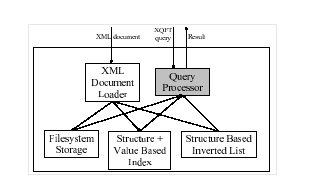
\includegraphics[width=0.5\textwidth]{img/quark_architecture.png}
  \caption{Quark architecture}
\end{figure}
Quark is an experimental full-text search engine capable of indexing and querying XML documents, and it uses the TexQuery query language (see below). Quark was developed as a research project at Cornell University by Jayavel Shanmugasundaram and his associates.
\begin{figure}[!h]
  \centering
    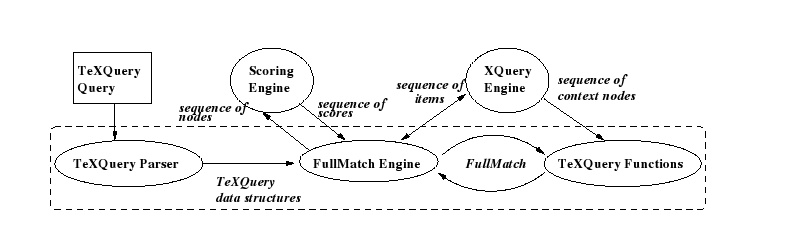
\includegraphics[width=1\textwidth]{img/texquery_architecture.png}
  \caption{TexQuery architecture}
\end{figure}
TexQuery is a query language extending upon Xquery with added full-text search capabilities. These extensions do not necessarily conform to the W3C recommendation, however TexQuery is an early precursor to the current W3C recommendation \cite{TEXQ00}, in whose development Shanmugasundaram actively participates.

\subsubsection{Galatex}
\begin{figure}[!h]
  \centering
    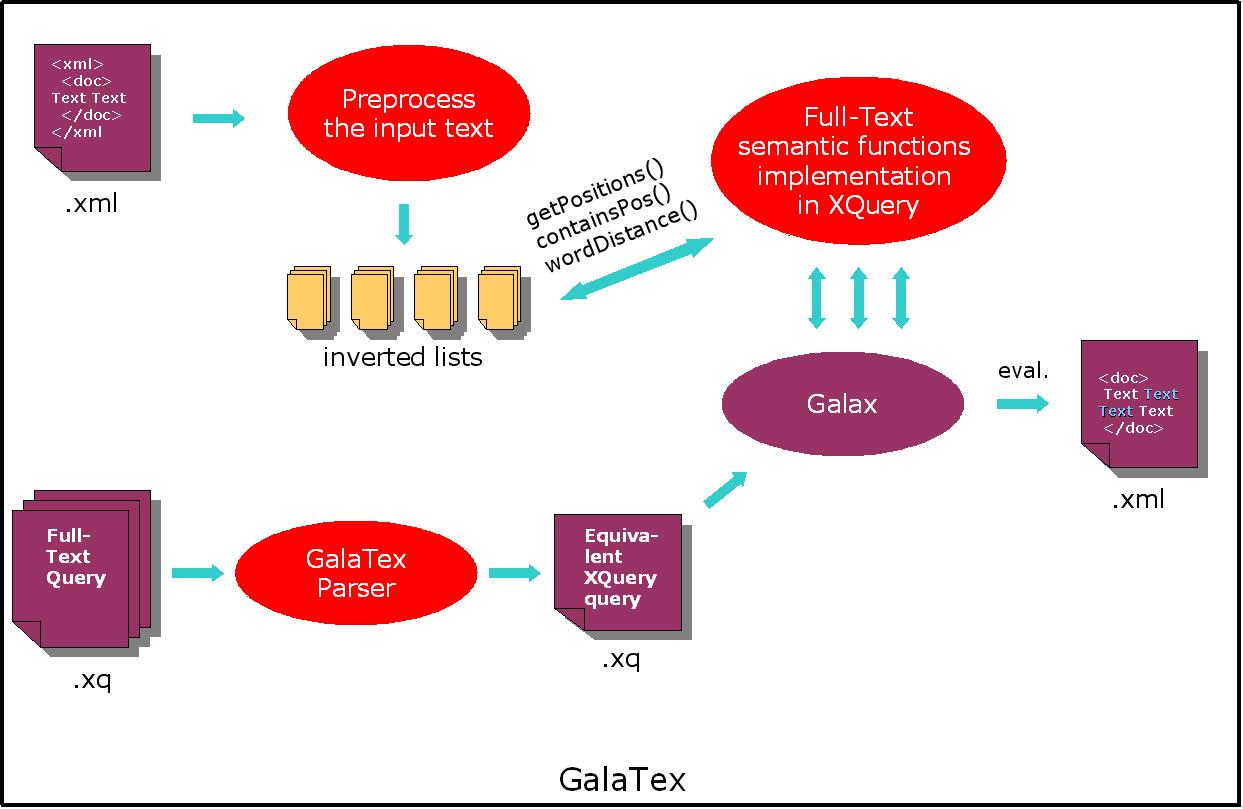
\includegraphics[width=1\textwidth]{img/galatex_architecture.png}
  \caption{Galatex architecture}
\end{figure}
GalaTex is a complete implementation of the Xquery 1.0 and Xpath 2.0
specifications with full-text extensions. GalaTex is an extension of Galax,
which is a generic Xquery engine. The XQFT query is parsed and converted to an
equivalent Xquery query which is passed to the Galax query engine. The GalaTex
source code is licensed under a non-commercial license developed to AT\&{}T 
\footnote{http://www.galaxquery.com/galatex/LICENSE} and is available at the
GalaTex website \cite{galatex}.

\subsubsection{Pathfinder}
\begin{figure}[!h]
  \centering
    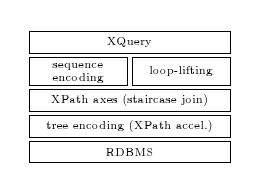
\includegraphics[width=0.5\textwidth]{img/pathfinder_architecture.png}
  \caption{Pathfinder architecture / development stack}
\end{figure}
The Pathfinder project is an XQuery parser running on top of relational database systems, namely MonetDB. The goal of the Pathfinder project is to investigate how relational database technology can be utilized to create a scalable and efficient XQuery implementation. However, the Pathfinder project has, at the current time of writing, no support for full text extensions. A future version of Pathfinder is planned to be capable of emitting SQL code generated from the XQuery parse tree. This illustrates the Pathfinder systems capabilities of interoperating with relational database systems.

Pathfinder is written in C, and the XQuery parser is a generated using standard Flex and Bison compiler generator tools.

\subsubsection{SaXon}
SaXon is an open source XSLT and XQuery processor. It is being actively developed by Michael Kay, and is licensed under the Mozilla Public License (MPL). SaXon conforms to the XSLT 2.0, XQuery 1.0 and XPath 2.0 recommendations by the W3C as of 23rd of january, 2007.

\subsubsection{Natix}
\begin{figure}[!h]
  \centering
    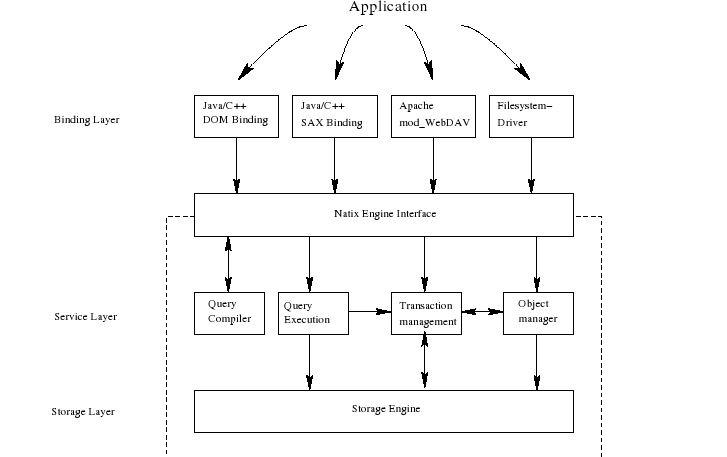
\includegraphics[width=1\textwidth]{img/natix_architecture.png}
  \caption{Natix architecture}
\end{figure}
Natix is an XML database system for persistent storage of XML, and provides access through DOM and SAX interfaces, as well as the option of performing XPath queries.

\section{Summary}
In this chapter, we have presented the basic facets of XQuery and XPath,
especially language features such as FLWOR constructs, path expressions, 
full-text extensions, and precedence. This creates a context for the subsequent
chapters where we will set out to create an XQuery parser with full-text
extensions. 

Further we have investigated existing implementations, both with and without
full-text extensions. These implementations will provide valuable points of
reference for our implementation in the following chapters.

In the next chapter, we will outline the architectural decisions made in this
project.
%Relasjonsalgebra
\chapter{Method}
\section{Parser construction}
Writing a parser from scratch was ruled out early for being too time consuming.
Instead it was decided to use tools for compiler and parser construction to
generate a parser from the XQuery 1.0 and XPath 2.0 grammar specifications
developed by the W3C.

\section{Evaluated alternatives}
\subsection{JFlex/CUP}
JFlex and CUP is a versatile combination consisting of JFlex which is a lexer
generator, and CUP which is a parser generator. These tools can be interfaced to
generate a complete parser with a separate lexical analyzer.

JFlex and CUP produces only LALR parsers, and since the W3C has specified an
LL(1) grammar for XQuery 1.0 and XPath 2.0, the combination of JFlex and CUP was
rejected from this project.

\subsection{JavaCC}
JavaCC could have been a viable alternative as it produces LL(k) parsers,
however compared to Antlr its grammar specification syntax deviated so much
from the W3C EBNF syntax, that grammar would have had to be extensively
rewritten.

\subsection{Antlr}
Antlr is a renowned tool for parser generation, and can generate LL(k) parsers.
Additionally, Antlr accepts a grammar specification syntactically very close to
the EBNF used by the W3C. This is the parser generater chosen for our project,
based on the criteria outlined in this section.

\section{Limitations in Antlr}
\subsection{Unicode}
It is important to note, however, that Antlr has limited support for unicode.
In this project this implies that our parser will not accept unicode characters
in the range from and above 0x10000. This will exclude the supplementary
multilingual plane (SMP) range of unicode characters, as well as the
supplementary ideographic plane (SIP) and the supplementary special-purpose
plane (SSP). These are seldomly used, but this is an important limitation
nonetheless. The Antlr developers have indicated that support for this unicode
range will be added in future versions of Antlr.

As a remedy for this situation it is possible to couple an external lexer with
Antlr which will accept unicode characters in the above mentioned character
ranges. For the sake of simplicity this has not been further investigated nor
implemented in this project.

\section{Rewriting the grammar for Antlr syntax conformity}
\subsection{Lexer vs. parser syntax}
The Antlr parser generator can generate parsers and lexers from a single grammar
file. The distinction between terminals and non-terminals is simply a matter of
convention, where terminals are assumed to start with uppercase letters, and
non-terminals are assumed to start with lowercase letters.

In the grammar specified by the W3C, all the productions (terminals and
non-terminals) all start with uppercase letters. Initially this caused some
confusion, because this grammar naturally generated a very big lexer and a very
small and non-functional parser.

This was mitigated by converting non-terminal productions to start with
lowercase letters.

\subsection{Rewriting the W3C 'dash' operator}
In their specification, the W3c uses a dash operator, which has the following
semantic meaning in a grammar (from \cite{w3c03}, section 6):
\begin{quote}
A - B: matches any string that matches A but does not match B.
\end{quote}
This operator is not supported in Antlr, so it was necessary to rewrite
these productions using \emph{semantic predicates} where necessary. Thankfully,
in the original specification, the usage of the dash operator was rather sparse
and only used in trivial productions.

An example of rewriting the dash operator using semantic predicates:
\begin{verbatim}
// Original production
piTarget : Name - (('X' | 'x') ('M' | 'm') ('L' | 'l'));

// Rewritten production using a semantic predicate
piTarget : n=Name { !$n.getText().equalsIgnoreCase("XML") }?;
\end{verbatim}
The original production can be interpreted as ``piTarget can be a Name, but not
`XML', regardless of character casing''. The syntactic predicate will imitate
this behaviour using the method equalsIgnoreCase(). As can be seen from this
example, a semantic predicate is simply any kind of boolean Java expression.
This is a flexible solution, because the boolean expression can be wrapped in a
method with boolean return type, which for example then can be placed inside a
@members { } clause in the grammar file, or even as a static method in an
external class. This makes it possible to add complex grammar logic without
disturbing grammar brevity, if necessary.

\subsection{Grammar LL(1) conformity}
The grammar specification given by W3C is in a very compact and non-verbose
form, annoted with links to certain constraints and issues that need to be kept
in mind by anyone seeking to write a parser for XQuery and XPath. Here we will
list these constraints and briefly explain their implications for the parser.

\begin{itemize}
  \item 
\end{itemize}

\subsection{Reserved keywords}
A particular feature in XQuery is the lack of reserved keywords. This creates a
series of problems when a lexer based on the verbatim grammar specification from
the W3C is trying to recognize tokens. The culprit is the ambiguously defined
terminal symbols. Some of the base character tokens intersect with each other
and makes it hard if not impossible for the lexer to distinguish two different
tokens composed of different token fragments with intersecting characters.

One possible solution to this problem was to eliminate ambiguities in the lexer.
This approach was tried by finding and removing duplicate characters from token
fragments, and then generalizing the tokens and adding semantic predicates to
check for illegal and/or missing characters.

TODO: example

TODO: result (also note in conclusion)

\subsection{Nested comments}
XQuery allows nested comments, for example:
\begin{verbatim}
(: this is a comment (: this comment is nested :) :)
\end{verbatim}
This is a classic problem in compiler construction, however it can be solved
using standard Antlr syntax, without resorting to custom functions/methods for
consuming input and keeping track of nesting. The original EBNF as specified by
W3C is as follows:
\begin{verbatim}
Comment ::= "(:" (CommentContents | Comment)* ":)"
\end{verbatim}
At first glance, this seems uncomplicated and straight forward, but this grammar
needs to be rewritten to be accepted by an LL(1) parser. A suggestion for a 
solution to this problem was initially found on the Antlr mailing
list\footnote{http://www.antlr.org:8080/pipermail/antlr-interest/2005-July/012967.html},
and we based our implementation on such an approach. This lexer rule will
correctly detect and allow nested comments, and hide them from the parser:
\begin{verbatim}	
Comment : LXQCOMMENTSi 
          (Comment | (COLONSi ~RPARSi)=>COLONSi 
          | (LPARSi ~COLONSi)=>LPARSi 
          | ~(LPARSi | COLONSi | IkkeChar))* 
          RXQCOMMENTSi {$channel=HIDDEN;};
\end{verbatim}
TODO: oppdater eksempelet over (IkkeChar)


\section{Unit testing the grammar}
Unit testing can be a powerful tool for asserting functionality and can be a
helpful aid in debugging and prevention of regression errors.  For unit testing the
grammar specification, gUnit \cite{gunit00} was employed. This tool uses a
syntax similar to Antlr itself, however instead of defining productions, one
defines a set of inputs for some rule, as well as the expected result. Consider
this example:

\begin{verbatim}
gunit XQFT;
@header{package no.ntnu.xqft.parse;}

piTarget: // Test piTarget rule

    // Any case permutation of 'XML' must fail
    "Xml" FAIL
    "XMl" FAIL
    "XML" FAIL
    "XmL" FAIL
\end{verbatim}

This is a complete input file for gUnit, and will automatically discover the
classes XQFTLexer and XQFTParser in the package no.ntnu.xqft.parse. gUnit will
then proceed to invoke the lexer with ``Xml'', ``XMl'', ``XML'', and ``XmL'' as
input, and pass the lexer to an instance of XQFTParser and execute the production
piTarget. For all these inputs, it will assert that the parser emits an error
(i.e it must fail to pass the test).

In case of a test where the parser should not fail, the syntax is as follows:
\begin{verbatim}
forClause:
	"for $a in document(\"abc.xml\")/a/b/text()" OK
\end{verbatim}
Here gUnit will assert that the parser will not fail for the given inpu (i.e it
must not fail to pass the test).

gUnit is also capable of parsing abstract syntax trees built by the generated
parser, but this feature has not been used in this project.

\section{Debugging}
There are several approaches to debugging. Antlrworks \cite{antlrwrks00} is a
simple tool for writing, testing and debugging Antlr grammars. The debugging
interface is useful in that it draws a realtime step-by-step parse tree as the
input is being parsed, as well as displaying a list of parser events.

\section{Scoping and symbol tables}
Scoping was implemented using a simple tree structure consisting of parent- and
child scopes. XQuery only allows new scopes to be defined through the
enclosedExpr production rule. This makes it trivial to start a new scope at the
beginning of a enclosedExpr, and end the scope and the end of an enclosedExpr.
This has been implemented as follows:
\begin{figure}[!h]
\begin{verbatim}
enclosedExpr : 
    LBRACESi {
        Scope parent = this.currentScope; 
        this.currentScope = new Scope(); 
        this.currentScope.setParent(parent); 
    }
    expr 
    RBRACSi { 
        this.currentScope = this.currentScope.getParent(); 
    }
;
\end{verbatim}
\caption{Scoping logic embedded in grammar definition}
\end{figure}

Where this.currentScope is a reference to the ``current'' scope in this
context. This member variable is initiated with an empty scope when an object
of the parser class is instantiated.

The implementation above (which is formatted slightly for brevity) will
automatically build a scope tree as the input is parsed.

The currentScope object, which is an object of type Scope, holds one reference
to a symbol table. The symbol table, which is a simple subclass of
java.util.HashMap, is not capable of performing symbol lookups throughout the
scope tree. This functionality is rather provided by the Scope class. This UML diagram
illustrates the relationship between the Scope, SymTab, and Symbol classes:
\begin{figure}[!h]
  \centering
    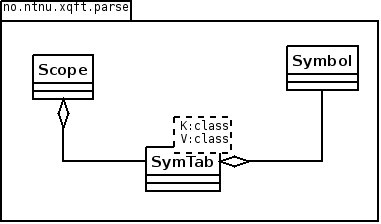
\includegraphics[scale=0.8]{img/uml1}
  \caption{Simplified UML overview of classes related to scope and symbol table}
\end{figure}

\section{Type checking}
XQuery/XPath has a well-defined type hierarchy:
\begin{figure}[!h]
  \centering
    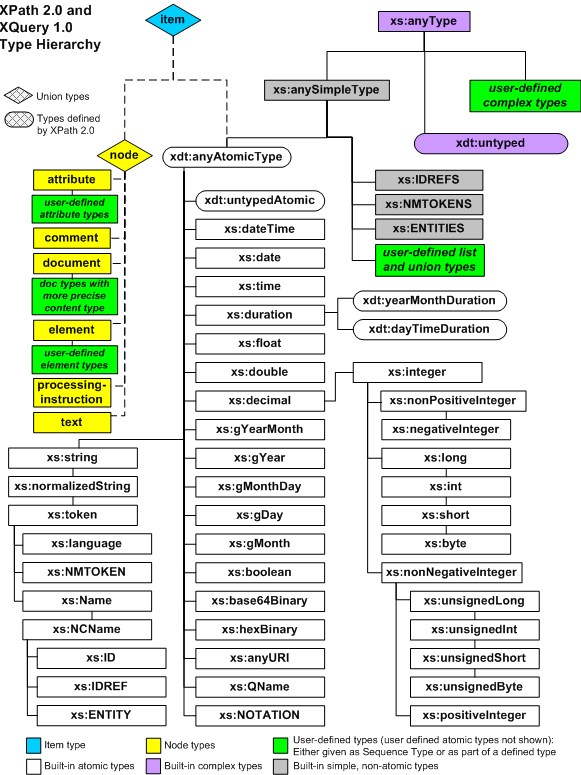
\includegraphics[scale=0.5]{img/xpathtypehierarchy}
  \caption{XQuery/XPath type hierarchy \cite{w3c04} (graphic copyright
  \copyright W3C)}
\end{figure}
All types are derived from the following types in the hierarchy:
\begin{itemize}
  \item Node types
  \item Structure types
  \item Atomic types
  \item Simple types
\end{itemize}

\chapter{The Parser Generator - ANTLR}
\label{sect:antlr}

\underline{\textbf{\LARGE //TODO:}} Hvorfor ANTLR?

ANTLR, Another Tool for Language Recognition, is a parser generator under a three clause BSD-license \cite{antlrorg}.  It is a successor of PCCTS, sometimes called ANTLR v1, and the latest version is ANTLR v3. PCCTS was developed by Professor Terrence Parr of the University of San Francisco, now the primus motor behind ANTLR.

ANTLR generates recursive-decent recognizers that utilizes predicated LL(*) -- an extension to LL(k) that uses arbitrary lookahead to make decisions. LL parsers are often said to be more intuitive and easier for humans to read than e.g. LALR parsers. This is supported by the fact that most hand written parsers are LL parsers. ANTLR supports multiple target languages, including Java. There are generally three types of recognizers ANTLR can generate: lexers, parsers and tree parsers/walkers.

\section{LL(*)}
The LL(*) parsing strategy is a strategy unique to ANTLR, invented by Terrence Parr for ANTLR v3. It is much more powerful than traditional LL(k) parsing \cite{definitiveAntlr}, because it is not limited to a finite amount of lookahead. It enhances the LL decision's predictive capabilities, but does not by means alter the recursive decent parsing strategy.  By automatically doing left-factoring LL(*) allows developers to write more natural and human readable grammar. If a grammar is specified as LL(k), LL(*) will degenerate into LL(k) for this grammar. A decision is LL(*) if a DFA exist that recognizes the decision's exact lookahead language and has the following \cite{definitiveAntlr}:
\begin{itemize}
\item No unreachable states
\item No dangling states, i.e. states that cannot reach an accept state
\item At least one accept state for each alternative.
\end{itemize}
All alternatives have a lookahead language, and if the lookahead languages of the alternatives are disjoint, the decision is LL(*). Except for not having a finite lookahead, LL(*) differs from LL(k) with backtracking in that it is looking ahead with the DFA, and not the whole parser. A thorough description of LL(*) can be found in \cite{lookahead}.

\section{Grammar Specification}
\label{sect:antlr:grammarSpec}
The grammar is specified in a type of extended Backus-Naur form (EBNF), where the extension from BNF consists of the Kleene operators $?$, $ +$ and $\ast$, and the not-operator $\sim$.  In addition, ANTLR introduces some types of predicates, namely validating, hoisting and gated semantic predicates and syntactic predicates. Validating and disambiguating semantic predicates is on the form \verb!{sem. predicate}?!, gated semantic predicates is on the form \verb!{sem. predicate}?=>! and syntactic predicates is on the form \verb!(syn. pred.)=>!.

Member methods and variables of the parser can be placed in a \verb!@members{! members \verb!}! construct, and the corresponding \verb!@lexer::members{! members \verb!}! for the lexer. Actions specified in the target language can be inserted at appropriate places in the production rules wrapped in \verb!{! and \verb!}!. 

Lexer productions and token names start with a capital letter, and parser productions do not. It is possible, and even common, to specify both the lexer and parser grammar in one file, thus ANTLR will determine which productions that belong to the lexer and the parser respectively by looking at the case of the first letter in the name of the production rules. An example of ANTLR grammar can be seen in figure \ref{code:simpleGrammar}. This grammar will generate a parser that recognizes input such as "John is 37 years old".
\begin{figure}[h!]
\begin{verbatim}
NAME     : ( 'a'..'z' | 'A'..'Z')+;  
AGE      : ('1'..'9')? ('1'..'9'|'0');
sentence :  NAME ' is ' AGE  ' years old';
\end{verbatim}
\caption{ANTLR grammar example}
\label{code:simpleGrammar}
\end{figure}

\section{Lexer}
\label{sect:antlr:lexer}
Lexers generated by ANTLR is by default a class derived from \verb!Lexer! (in the \verb!org.antlr.runtime! package) with additional per lexer rule methods for matching incomming character data. The lexer depends upon a input module that implements the \verb!CharStream! (e.g. \verb!AntlrStringStream!) interface which defines the method \verb!public int LT(int k)!. This method returns the character in the input stream \verb!k! positions from the current position. The method \verb!public Token nextToken()! in the lexer will generate and return the next token found by the lexer in the character stream. An overview of this method can be seen in figure \ref{fig:nextToken}, where \verb!Lexer! is \verb!org.antlr.runtime.Lexer! and \verb!TestLexer! is the lexer generated by a fictional grammar \verb!Test!.

\begin{figure}[h]
\centering
\begin{tabular}{|l|l|l|} \hline
\textbf{Lexer} 				& \textbf{TestLexer} 			\\ \hline
\verb!CharStream input;!		& 					\\
					&					\\
\verb!nextToken(){!			&					\\
\verb!   token = NULL;!			&					\\
\verb!   pos = input.position!		&					\\
\verb!   text = NULL;!			&					\\
					& \verb!mTokens{!			\\ 
					& \verb!   _type = "predict type"!	\\
					& \verb!   input.updatePosition()!	\\
					& \verb!   this.type = _type;!		\\
					& \verb!}!				\\
\verb!   if(token == NULL){!		&					\\
\verb!     emit(){!			&					\\
\verb!        t=new Token(type, pos,! 	&					\\
\verb!            input.position, input);!&					\\ 
\verb!        t.setText(text)!		&					\\
\verb!        emit(t){!			&					\\
\verb!          token=t;}!		&					\\
\verb!     }!				&					\\
\verb!   }!				&					\\
\verb!   return token;!			&					\\
\verb!}!				&					\\ \hline
\end{tabular}
\caption{Pseudocode showing how the lexer generates tokens.}
\label{fig:nextToken}
\end{figure}
Unless explicitly defined the tokens will hold the text they have matched as \verb!input!, \verb!startPosition! and \verb!endPosition!. It is also worth noticing that \verb!token! is set to \verb!NULL! for each token request, and a token will only be generated by \verb!nextToken()! if \verb!token! still has the value \verb!NULL! after the generated part of the lexer has decided which token to match.

When the lexer is to predict which type of token it should return (\verb!"predict type"! in figure \ref{fig:nextToken}), it peeks into the input character stream as many positions ahead needed to disambiguate the alternatives and make a decision. However, for e.g. to easily be able to define keywords, some ambiguous alternatives are allowed. ANTLR will then choose between the alternatives following some simple rules:
\begin{itemize}
\item An explicit expressed character sequence is chosen before an implicit one.
\item A longer sequence is chosen before a shorter one.
\item A production declared before another is chosen first.
\end{itemize}
These rules are ranked, and ANTLR will only use as many of them needed to differanciate the alternatives. Syntactic and semantic predicates will also make an impact on the decisionmaking as seen later. Figure \ref{fig:grammarPrec} shows a grammar with ambiguous alternatives, a simplified version of the code generated can be seen in figure \ref{fig:codeGenerated} where you can see that the parser will choose \verb!AB! before \verb!A! (and thus \verb!A B!) and \verb!A! before \verb!ANY!.
\begin{figure}[h!]
\begin{verbatim}
A       : 'a';
B       : 'b';
AB      : 'ab';
ANY     : ('a'..'z')+;
\end{verbatim}
\caption{Grammar showing the precidence among rules}
\label{fig:grammarPrec}
\end{figure}

\begin{figure}[h!]
\begin{verbatim}
int alt = 4;
if(LA(1) == 'a')
      if(LA(2) == 'b')
            if(LA(3) >= 'a' && LA(3) <= 'z')
                  alt = 4;
            else
                  alt = 3;
      else
            alt = 1;
else if(LA(1) == 'b')
      if(LA(2) >= 'a' && LA(2) <= 'z')
            alt = 4;
      else
            alt = 2;
else if(LA(1) >= 'c' && LA(1) <= 'z')
      alt = 4;
else
      throw new NoViableAltException();
\end{verbatim}
\caption{Example of how ANTLR predicts token type.}
\label{fig:codeGenerated}
\end{figure}
Production rules declared with the keyword \verb!fragment! are rules that never will be implicitly considered as an alternative. Fragment rules depend upon being referenced by other rules, fragment or not.
If the lexer grammar is so big that it may not compile, ANTLR will substitute the inline DFAs with DFA objects for prediction. These objects are implemented as a set of transition tables. More about the DFA objects can be found in \cite{antlrCodeGen}.

\section{Parser}
\label{sect:antlr:parser}
The parser generated by ANTLR is very much analogous with the lexer. By default the parser will be derived from \verb!org.antlr.runtime.Parser!. In addition to the methods and variables inherited, the generated parser will contain one method per production rule in the parser grammar. The parser does not have one defined "starting rule", thus, each method will have a prediction algorithm similar to \verb!mTokens()! in the lexer. As with the lexer, the algorithm peeks into the input stream as many tokens forward needed to differentiate between the alternatives. The parser takes a object that implements \verb!TokenStream! as input, which again takes a \verb!TokenSource! (the base class of \verb!Lexer!) as input. \verb!TokenStream! contains a method \verb!LT(int k)!, and classes that implements this interface often include a method \verb!LA(int k)! which returns the type of the token returned by the other method. \verb!CommonTokenStream! is a simple implementation of \verb!TokenStream!, and recomended by the ANTLR Community \cite{antlrorg} in most cases. The first time the \verb!LA(int k)! method of \verb!CommonTokenStream! is called a buffer of tokens will be filled by calling the lexer's \verb!nextToken()! until it returns \verb!Token.EOF! -- the end of the input. This means that before the parser starts to try matching production rules, the lexer will be finished creating tokens. Parsing will commence by calling the method created for the top-most production in the grammar, which in the case of XQuery with full text extension is \verb!module()!.

\section{Generating an Abstract Syntax Tree}
\label{sect:antlr:ast}
By default, ANTLR will not generate an AST from the grammar specification.
However, by setting the \verb!output! option value to \verb!AST! in the grammar
header, ANTLR will generate a simple ``flat'' linked list consisting of all the
parsed tokens in the input. 

This flat AST can be structured by adding operators and rewrite rules to tell
ANTLR which tokens to use as root nodes in productions, and which to leave out
of the AST entirely. There are two primary operators for AST structuring, hat
(\^{}) and exclamation mark (!). These operators are postfixed to tokens to
promote them to root nodes and exclude them completely from the AST,
respectively. Figure \ref{code:astOperators} shows an example where the
paranthesis would be excluded from the AST, and the \verb!PLUS! token
would be promoted to root node with two \verb!expr! children.

\begin{figure}[h!]
\begin{verbatim}
sum : '('! expr PLUS^ expr ')'!;
\end{verbatim}
\caption{Simple AST structuring operators example}
\label{code:astOperators}
\end{figure}

Additionally, ANTLR provides the commodity of rewrite rules for tailoring AST
generation. Figure \ref{code:astRewriteRules} shows an example with a rule for
an if-statement. The ``arrow'' (->) marks the start of the rewrite rule. The hat
(\^{}) operator indicates that the first token in the list should be promoted to
root node. There is no need to use exclamation marks as simple omission will
leave unwanted tokens out of the AST. Also note that variables can be used
exactly like in grammar predicates.

\begin{figure}[h!]
\begin{verbatim}
if : 'if' expr 'then' s1=stmt 'else' s2=stmt 'endif'
     -> ^(IFEXPR expr $s1 $s2);
\end{verbatim}
\caption{Usage of simple AST rewrite rules}
\label{code:astRewriteRules}
\end{figure}

Sometimes it may be necessary to customize the AST by adding custom fields to
the nodes or performing certain operations on them not supported by the built-in
tree representations. This can be done by subclassing the BaseTree (or
CommonTree) classes as well as adding a custom tree adaptor class, and setting
the option \verb!ASTLabelType=MyCustomTreeClass! in the grammar file header.

\section{Semantic Predicates}
\label{sect:antlr:semantic_preds}
Even though LL(*) allows the parser to scan arbitrarily far forward for any symbol or sequence of symbols to distinguish alternatives, it still has some weaknesses - particularly so when it comes to recursive rules. Semantic predicates are boolean expressions evaluated during runtime used to specify the semantic validity of an alternative. Predicate in this case simply means conditional, and the term semantic implies you are talking about arbitrary boolean expressions rather than a syntactic condition.  As previously mentioned, ANTLR provides three types of semantic predicates:
\begin{itemize}
\item Disambiguating semantic predicates; which disambiguate syntactically identical alternatives.
\item Gated semantic predicates; which can dynamically turn on and off parts of the grammar.
\item Validating semantic predicates; which throw a recognition exception if the predicate fails.
\end{itemize}

\subsection{Validating Semantic Predicates}
\label{sect:antlr:val_semantic_preds}
If the expression being evaluated in a validating semantic predicate yields $false$, an exception is thrown, expressing that a semantic predicate has failed. These predicates are never included in the decision-making process. Validating semantic predicates can be very handy in cases where e.g. you want to restrain the possible values a tokens can have, or to check if a variable is being referenced before its declaration. An example of a validating semantic predicate can be seen in figure \ref{code:validateSemantic}.

\begin{figure}[h!]
\begin{verbatim}
expr    : N {Integer.parseInt($N.getText()).intValue() < 7}?
        | . . .
        ;
\end{verbatim}
\caption[Validating semantic predicate.]{A Validating semantic predicate checking if the number value of \texttt{N} is less than $7$.}
\label{code:validateSemantic}
\end{figure}
As can be seen from this example, a semantic predicate is simply any kind of boolean Java expression. This is a flexible solution, because the boolean expression can be wrapped in a method with boolean return type, which for example then can be placed inside a @members { } clause in the grammar file, or even as a static method in an external class. This makes it possible to add complex grammar logic without
disturbing grammar brevity, if necessary.

\subsection{Disambiguating Semantic Predicates}
\label{sect:antlr:disambiguatingSemantic}
Disambiguating semantic predicates are hoisted into the prediction decisions of the LL(*) recognizer, but only if no decision can be made by syntax alone. There are generally two cases where these types of predicates are really useful: when a property of a token must dictate how the parser interprets it, and when a surrounding construct or some runtime information should alter how the parser matches the current construct. In most cases when a validating semantic predicate is applied, it can be transformed into a disambiguating semantic predicate. This will result in a syntax error instead of an exception if the predicate evaluates to $false$.

To fully resolve a non-determinism with disambiguating semantic predicates, all alternatives that contribute to the non-determinism will have to be covered, as seen in figure \ref{code:disambigSemantic}. The DFA generated in figure \ref{code:disambigSemantic} is illustrated in figure \ref{fig:dfaDisambiguate}.

\begin{figure}[h!]
\begin{verbatim}
expr      : {pred1}? A 
          | {pred2}? A
          ;
\end{verbatim}
\caption{Disambiguating semantic predicates.}
\label{code:disambigSemantic}
\end{figure}

\begin{figure}[!h]
  \centering
    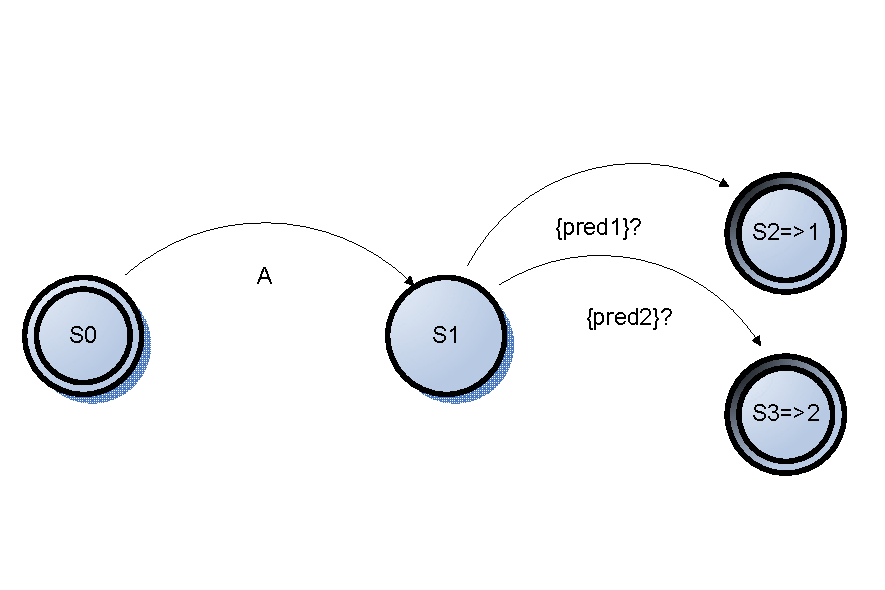
\includegraphics[scale=0.6]{img/disambigsemantic}
  \caption{The DFA of figure \ref{code:disambigSemantic}}
  \label{fig:dfaDisambiguate}
\end{figure}
As mentioned earlier, ANTLR hoists disambiguating semantic predicates into the state where the alternative prediction is made, which can be illustrated by the fact that the grammar inn figure \ref{code:disambigSemanticHoist} also yields the DFA shown in figure \ref{fig:dfaDisambiguate}. This includes only the predicates visible at the left edge of the production rule. 
\begin{figure}[h!]
\begin{verbatim}
expr      : a 
          | b
          ;
a         : {pred1}? A ;
b         : {pred2}? A;
\end{verbatim}
\caption{Hoisted disambiguating semantic predicates.}
\label{code:disambigSemanticHoist}
\end{figure}
Predicates implicitly specify precedence among the alternatives, where an earlier specified alternative has precedence over a later one. If both \verb!pred1! and \verb!pred2! would evaluate to true in figure \ref{code:disambigSemantic}., the first \verb!A! would be matched. In the case of only the first $n-1$ non-deterministic alternatives among $n$ are covered by a semantic predicate, the $n$th alternative would be covered with a \verb!{true}?! predicate. However, if this uncovered alternative was places first, it would be covered by a predicate that is the complement of the union of the following $n-1$ predicates.

\subsection{Gated Semantic Predicates}
\label{sect:antlr:gate_semantic_preds}
Gated semantic predicates are used when it is desirable to turn parts of a grammar on or off based on runtime information. The predicate will be hoisted into the decision even if the decision is deterministic by considering syntax alone. The difference between gated and disambiguating semantic predicates is that decisions use disambiguating semantic predicates only when syntax alone is insufficient to distinguish between alternatives. Figure \ref{code:gatedSemantic} shows an example of a gated semantic predicate, the resulting DFA is illustrated in figure \ref{fig:dfaGated}, showing how the predicate is hoisted even with no syntactic ambiguity.

\begin{figure}[h!]
\begin{verbatim}
expr      : a 
          | b
          ; 
a         : A;
b         : {pred}?=>B;
\end{verbatim}
\caption{Gated semantic predicate.}
\label{code:gatedSemantic}
\end{figure}

\begin{figure}[!h]
  \centering
    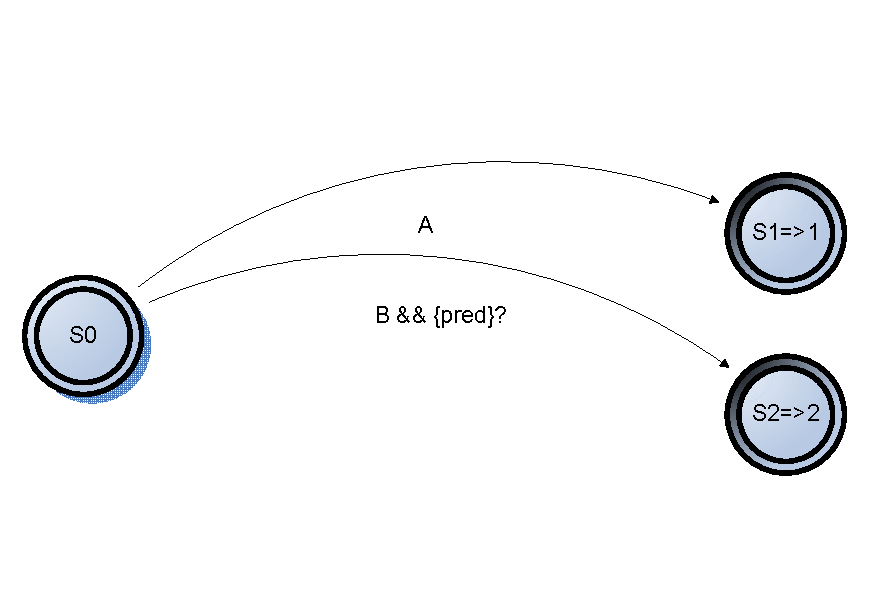
\includegraphics[scale=0.6]{img/gatedsemantic}
  \caption{The DFA of figure \ref{code:gatedSemantic}}
  \label{fig:dfaGated}
\end{figure}

\section{Syntactic Predicates}
\label{sect:antlr:syntacticPredicate}
Syntactic predicates are similar to semantic predicates except that they specify the syntactic validity of applying an alternative rather than the semantic validity. As with the semantic predicates their syntactic counterparts alter the parse based upon information available at runtime, but the only information the syntactic predicates use are future input symbols.  Both syntactic predicates and LL(*) support arbitrary lookahead, but whereas LL(*) uses a DFA to examine the future input symbols, the predicates use a pushdown machine, making them capable of recognizing more complicated structures in the lookahead than DFAs. Syntactic predicates are especially useful to specify the precedence between to ambiguous alternatives, or when LL(*) cannot handle the grammar the way you would like to write it.

When used to disambiguate between alternatives, ANTLR will try the alternatives in order. The alternative whose predicate is the first to return true, is the one chosen ("if it looks like A, it is A"). In its simplest form, syntactic predicates can be used to look ahead an arbitrarily number of symbols, to check if they match the symbols specified in the predicate. In a case like this ANTLR rewrites the predicate to a gated semantic predicate, an example of this is the grammar in figure \ref{code:syntactic} being translated to the equivalent grammar of figure \ref{code:translatedSyntactic}.

\begin{figure}[h!]
\begin{verbatim}
expr      : (A)=> A 
          | B
          ; 
\end{verbatim}
\caption{Syntactic predicate.}
\label{code:syntactic}
\end{figure}
\begin{figure}[h!]
\begin{verbatim}
expr      : {input.LA(1)==A}?=>A 
          | B
          ; 
\end{verbatim}
\caption{Translated syntactic predicate}
\label{code:translatedSyntactic}
\end{figure}

In more complex cases, syntactic predicates are implemented as disambiguating semantic predicates that invoke parser backtracking methods. These methods compare the input stream with the symbols specified in the predicate. If the stream and the symbols match, the method returns true, and the input stream is rolled back to the place where the comparing started. Such a case is exemplified by figure \ref{code:complexSyntactic}, where with an input such as "((a))" ANTLR will try the second alternative, succeed, backtrack, before telling the parser to choose this alternative.
\begin{figure}[h!]
\begin{verbatim}
expr      : (simple)=> simple ';'
          | (recur)=> recur ';'  
          | simple '!'
          ;
simple    : '(' ID ')';
recur     : '(' recur ')'
          | ID
          ;
ID        : ('a'..'z')+;
\end{verbatim}
\caption{A syntactic predicate which may backtrack}
\label{code:complexSyntactic}
\end{figure}

\section{Limitations in ANTLR}
\label{sect:parserconstructanddebug:limitations}
It is important to note, however, that ANTLR has limited support for unicode.
In this project this implies that our parser will not accept unicode characters
in the range from and above 0x10000. This will exclude the supplementary
multilingual plane (SMP) range of unicode characters, as well as the
supplementary ideographic plane (SIP) and the supplementary special-purpose
plane (SSP). These are seldomly used, but this is an important limitation
nonetheless. The Antlr developers have indicated that support for this unicode
range will be added in future versions of Antlr.

As a remedy for this situation it is possible to couple an external lexer with
ANTLR which will accept unicode characters in the above mentioned character
ranges. For the sake of simplicity this has not been further investigated nor
implemented in this project.

\section{Summary}
In this chapter we have presented our parser generator of choice, ANTLR. With a rich set of grammar specification operators, ANTLR supports most grammars with only little rewriting needed. But its real power comes in the form of the LL(*) capabilities and particulary the various forms of predicates. 

\underline{\textbf{\LARGE //TODO:}} Hva byr ANTLR p\aa ?

\chapter{Implementation}
\label{chapter:implementation}
This chapter describes the steps made to implement a proof of concept (dubbed
``the prototype'') which utilises some of the most important translation
rules developed in chapter \ref{chapter:translation}. This includes an overall system
description, as well as details about usage of the XQFT Parser. Furthermore, we
describe the process of building a MQL algebra tree, and how the context
sensitive visitor pattern is used. The scoping and symbol table implementation
is covered, as well as how metadata is passed between nodes while parsing the
syntax tree during the construction of the MQL tree. Finally, this chapter describes in
detail how some of the rules from the ``Tainting Dependencies'' method are
implemented and how they can be made to work in a real-life situation.

\section{Prerequisites}
As requested specifically by Fast Search \& Transfer, this proof of concept was implemented
in Java 5.0, using regular object oriented techniques, and is licensed under a
liberal BSD license. Instructions for compilation and installation can be
found in appendix \ref{appendix:installation}.

\section{List Of Supported Features}
This implementation supports the translation of the following XQuery features,
here annotated with references to the descriptions of their respective
translation:
\begin{itemize}
  \item FLWOR constructs (section \ref{sect:trans:TD:simpleFLWOR}, page
  \pageref{sect:trans:TD:simpleFLWOR})
  \item Sequence construction (section \ref{sect:trans:TD:seqBuild}, page
  \pageref{sect:trans:TD:seqBuild})
  \item Integer literals (section \ref{sect:trans:TD:literal}, page
  \pageref{sect:trans:TD:literal})
  \item Conditional expressions (section \ref{sect:trans:TD:ifThenElse}, page
  \pageref{sect:trans:TD:ifThenElse})
  \item Binary comparison (section \ref{sect:trans:TD:logical}, page
  \pageref{sect:trans:TD:logical})
\end{itemize}

\section{Overall system description}
A simplified class diagram describing the essentials of the system is shown in
figure \ref{fig:impl:sys:uml_complete}. The individual parts are described in
detail in the following sections of this chapter. In this section, the overall
system, flow of data, and external API is described.

It is important to note that, as mentioned, this implementation is a ``proof of
concept'' and only implements a subset of Tainting Dependencies described in chapter
\ref{chapter:translation}.

\begin{figure}[!htp]
\begin{center}
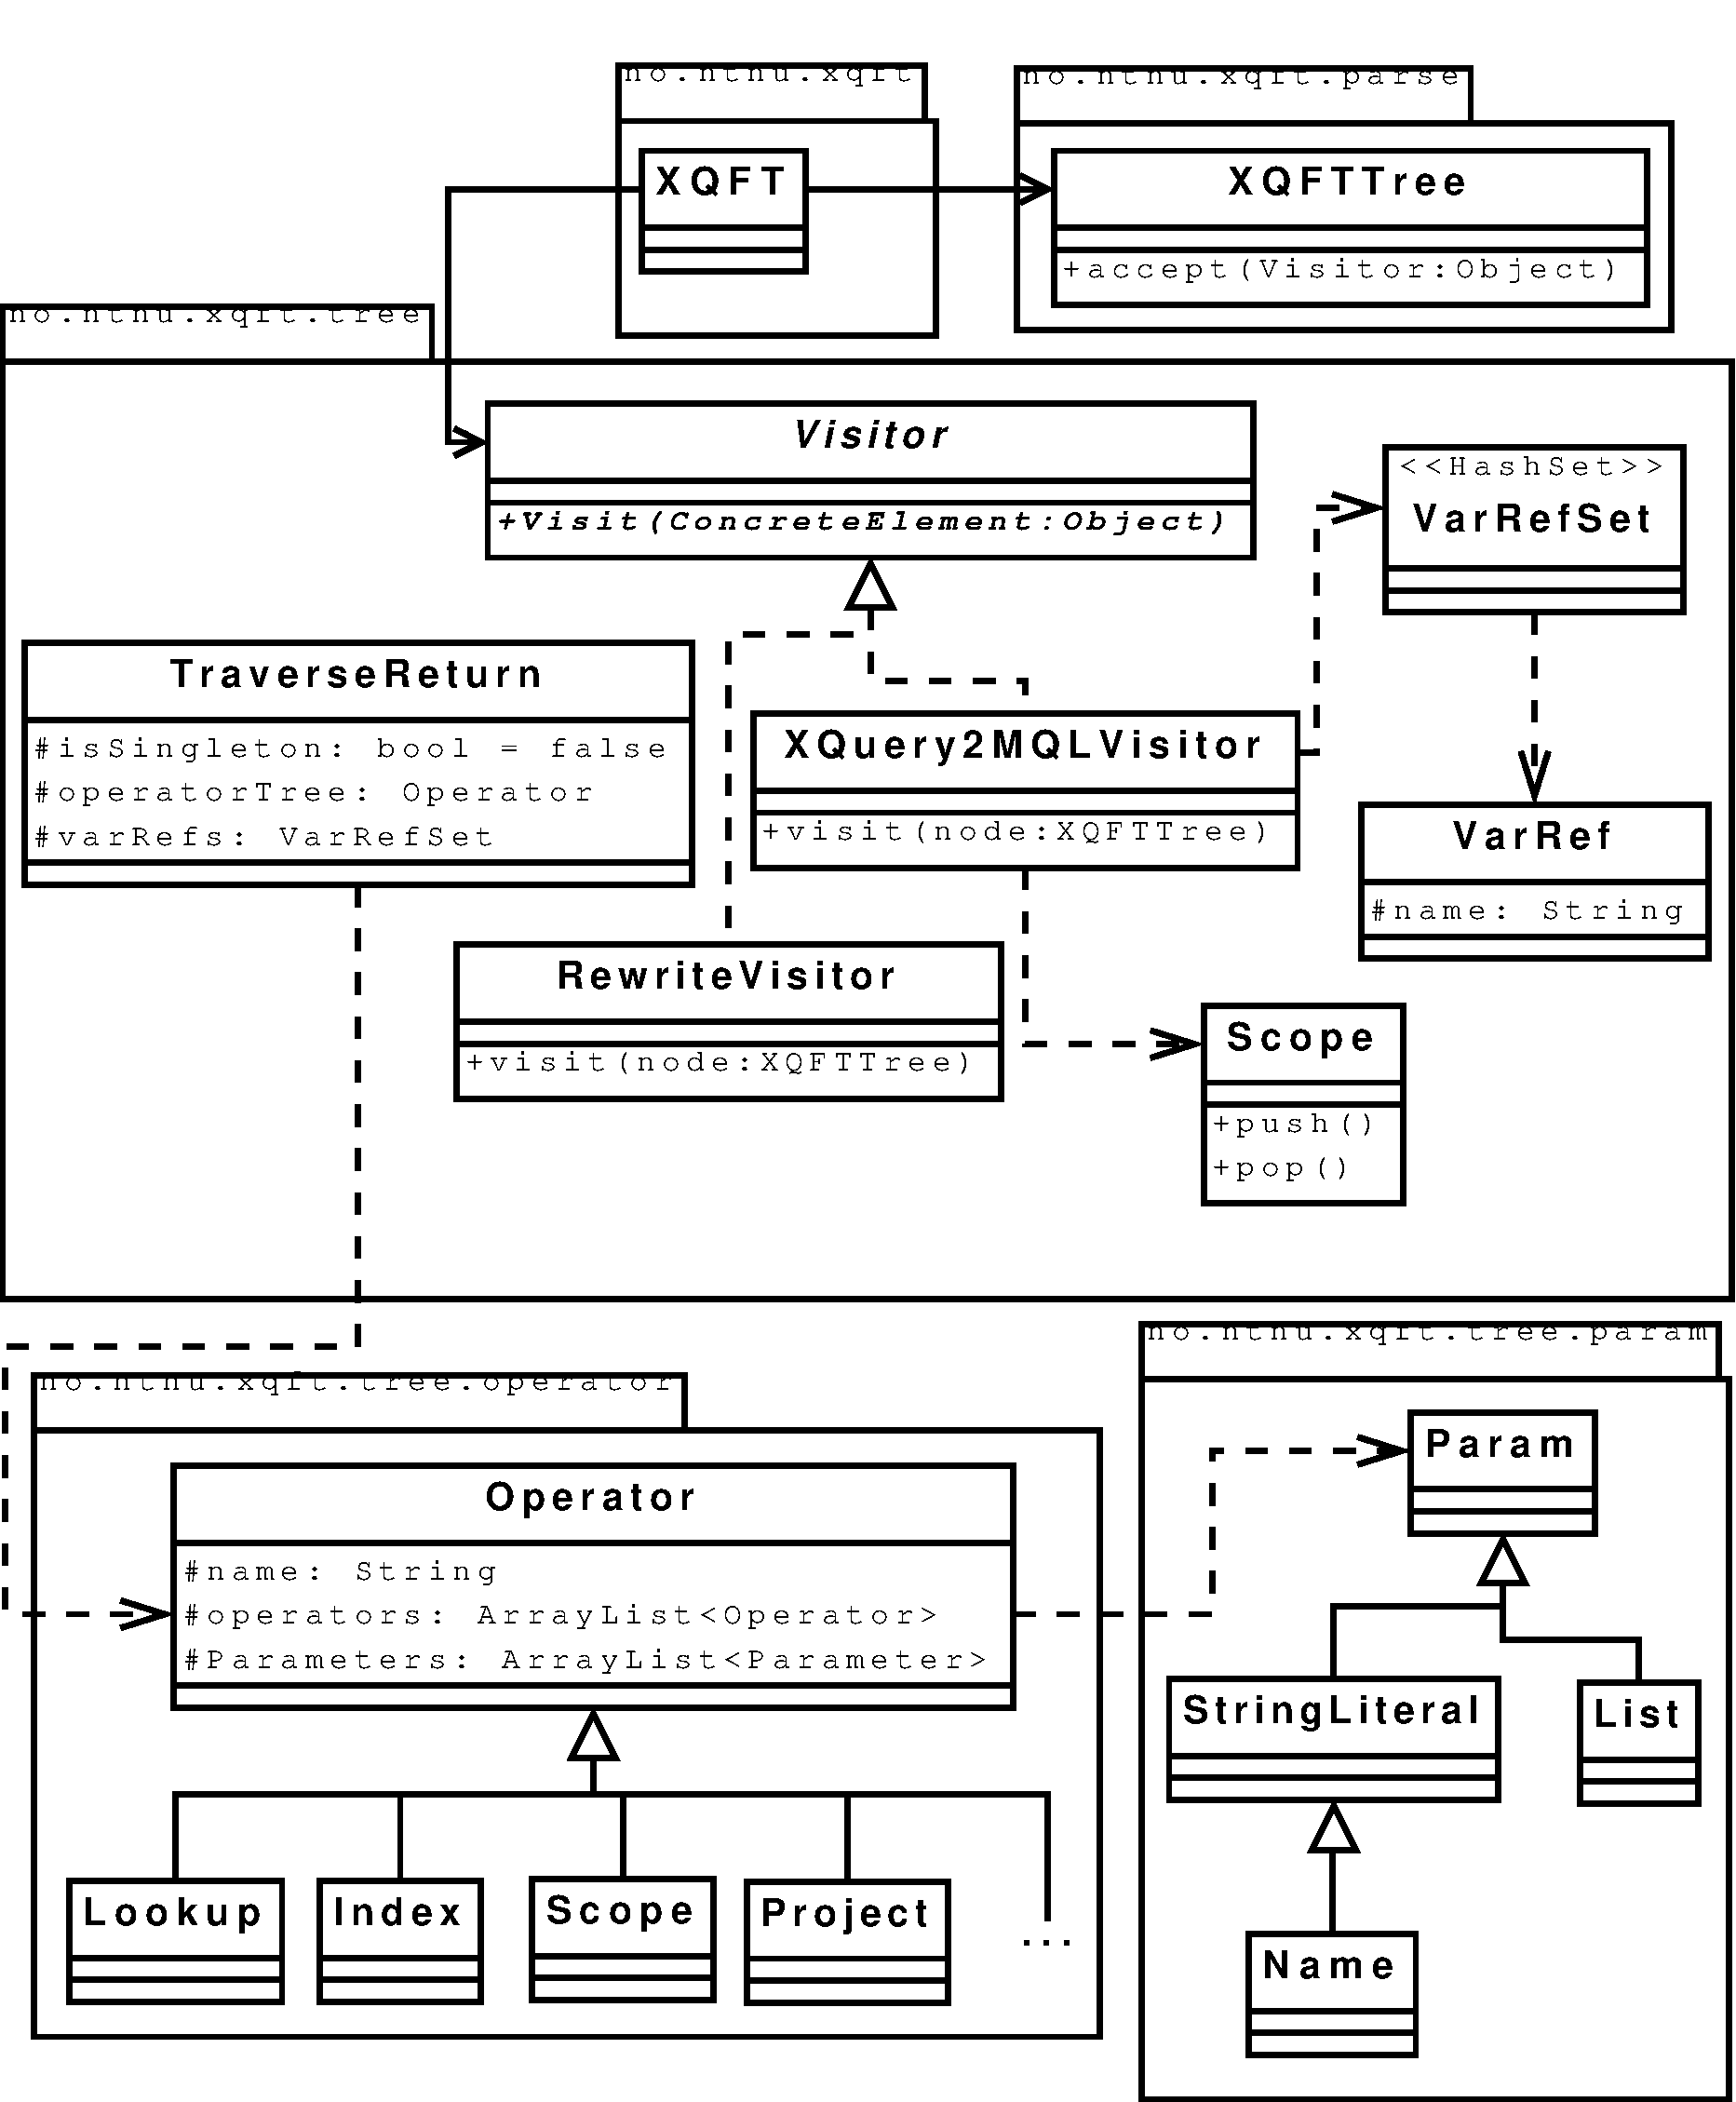
\includegraphics[scale=0.40]{diagrams/complete_uml}
  \caption{Simplified UML for complete implementation}
  \label{fig:impl:sys:uml_complete}
\end{center}
\end{figure}

\subsection{Data flow}
Figure \ref{fig:impl:sys:mql_dataflow} illustrates the flow of data when
translating a XQuery query into a MQL query (see section \ref{sect:method:mql}
on page \pageref{sect:method:mql} for a description of MQL). 

\begin{figure}[!htp]
\begin{center}
  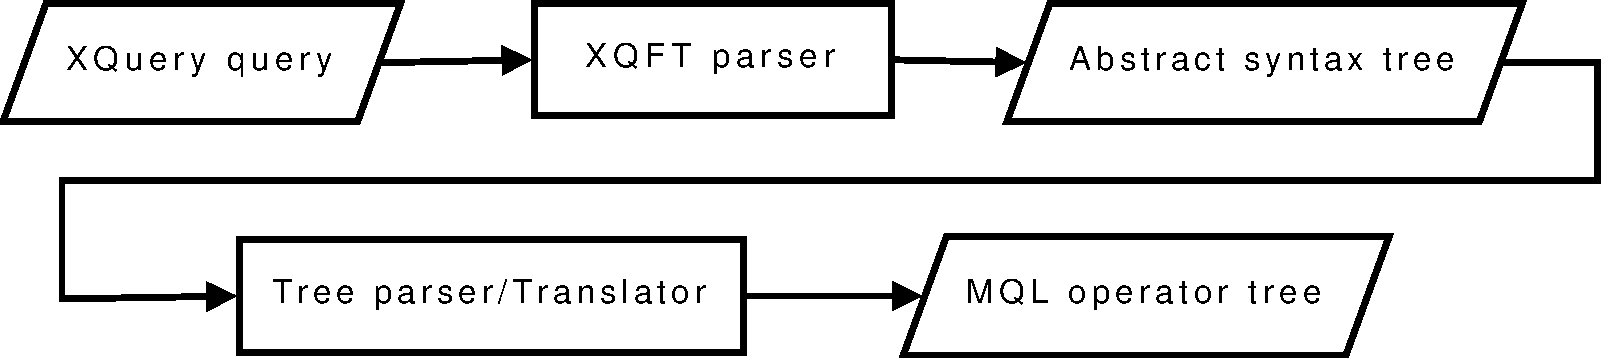
\includegraphics[scale=0.5]{diagrams/mql_dataflow}
  \caption{Data flow for XQuery parsing and translation to MQL}
  \label{fig:impl:sys:mql_dataflow}
\end{center}
\end{figure}

\subsection{Visible external API}
The API available to programmers is defined in a trivial manner in the
\texttt{no.ntnu.xqft.XQFT} class. This class can also be executed as a
standalone application (see next subsection). Figure
\ref{fig:impl:sys:xqft_extapi_uml} describes the \texttt{no.ntnu.xqft.XQFT}
class.

\begin{figure}[!htp]
\begin{center}
  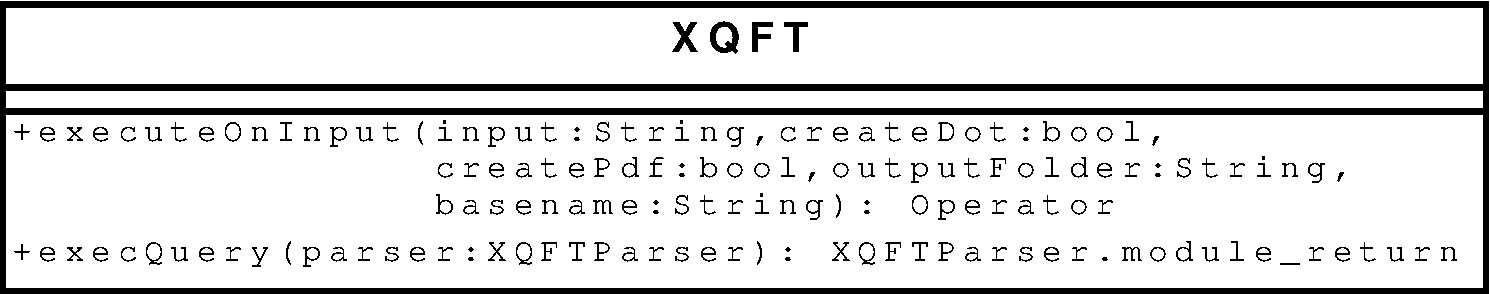
\includegraphics[scale=0.5]{diagrams/xqft_extapi_uml}
  \caption{External API for the XQuery to MQL translator}
  \label{fig:impl:sys:xqft_extapi_uml}
\end{center}
\end{figure}

As can be seen, two methods are primarily available. Out of these two,
\texttt{executeOnInput()} is the most complex, but also the most flexible. A
typical usage scenario for an external user could be as follows:

\begin{Verbatim}
XQFT xqft = new XQFT();
Operator mqlTree = xqft.executeOnInput(
                       "for $i in (1,2,3) return $i", 
                       false, false, null, null
                   );
\end{Verbatim}

The \texttt{mqlTree} would now be a reference to a complete MQL operator tree,
provided that no errors occured during the parse process or the translation
process.

\subsection{Command line interface}
\label{sect:impl:system:cli}
The command line interface is available by executing the
\texttt{no.ntnu.xqft.XQFT} class as a main class, as mentioned in the previous
section. The command line interface uses the Args
Engine\footnote{http://www.adarshr.com/papers/args} for the sake of simplicity
to parse options/switches on the command line. 

The command line usage is as follows:

\begin{verbatim}
java no.ntnu.xqft.XQFT [-p] [-t] [-o <path>] file1 file2 ... fileN
\end{verbatim}

It is also possible to specify queries in the form of strings enclosed in
double quotes, or any mix of strings and filenames. The switches are:
\begin{itemize}
  \item \texttt{-t} : output a DOT tree (requires graphviz)
  \item \texttt{-p} : output a PDF syntax tree (requires graphviz)
  \item \texttt{-o} \texttt{<path>} : stores generated PDF/DOT files in the given folder, 
  otherwise in the current folder (simply \texttt{./})
\end{itemize}

See appendix \ref{appendix:installation} for more information about installation and
dependencies.

\section{Using the XQFT Parser}
The \textit{XQFT Parser}\cite{ourselves} (described in section
\ref{sect:theory:xqftparser}) is a prerequisite for providing the abstract
syntax tree for this XQuery translator. This section will outline how this
parser was used and interfaced with the implementation.

\subsection{Basics and API}
The \textit{XQFT Parser} is a parser generated by the ANTLR parser generator.
Thus, there is a loosely standardised API available for any implementor
utilising a parser generated by ANTLR. In the case of \textit{XQFT Parser}, two
classes are generated: \texttt{XQFTParser} and \texttt{XQFTLexer}. These
classes are used in conjunction on an input string to produce an abstract syntax
tree (see next subsection, and also section
\ref{sect:theory:xqftparser:ast_construction}).

A typical use case to achieve this is shown in figure \ref{}

\begin{figure}[!htp]
\begin{center}
  \begin{Verbatim}
    CharStream cs 
        = new ANTLRStringStream(
            "for $i in (1,2,3) return $i");

    XQFTLexer lexer = new XQFTLexer(cs);

    UnbufferedCommonTokenStream tokens 
        = new UnbufferedCommonTokenStream();
	tokens.setTokenSource(lexer);

    XQFTParser parser = new XQFTParser(tokens);
    parser.setTreeAdaptor(new XQFTTreeAdaptor());
    parser.setLexer(lexer);

    XQFTTree ast = parser.module().getTree();
  \end{Verbatim}
  \caption{Using the XQFTParser and XQFTLexer classes}
  \label{figure:impl:using_xqft}
\end{center}
\end{figure}

\subsection{The XQFTTree class}
\subsection{Interfacing the XQFT Parser}
\section{Constructing the MQL algebra tree}
\label{sect:impl:construct_mql}
The MQL queries are constructed as a tree of operators bottom-up while parsing
the abstract syntax tree (for the corresponding XQuery query). 

\subsection{Operators and parameters}
\begin{figure}[!htp]
\begin{center}
  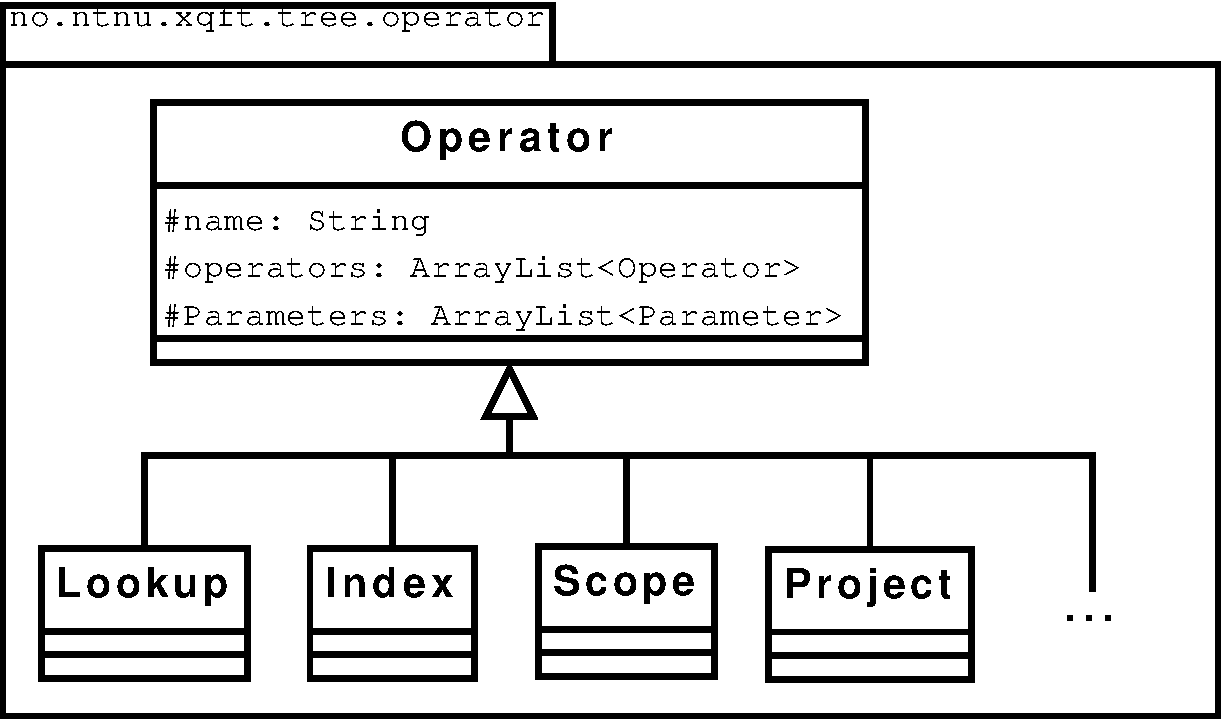
\includegraphics[scale=0.5]{diagrams/mql_operator_uml}
  \caption{Simplified class diagram of MQL operators}
  \label{fig:impl:mql_op_uml}
\end{center}
\end{figure}
The operators modeled in the implementation correspond to the operators
described in section \ref{sect:method:marsOperators}. A simplified class
diagram is shown in figure \ref{fig:impl:mql_op_uml}. Note that the
responsibility with regards to converting an operator to a string
representation is largely left to the various subclasses. However, the default
fallback for the \texttt{Operator} class is to return a string of the form
\begin{Verbatim}
operator_name(param1, param2, ..., paramN; 
              operator1, operator2, ..., operatorM)
\end{Verbatim}
This is sufficient in some cases, such as for the model of the \texttt{cross()}
operator.

\begin{figure}[!htp]
\begin{center}
  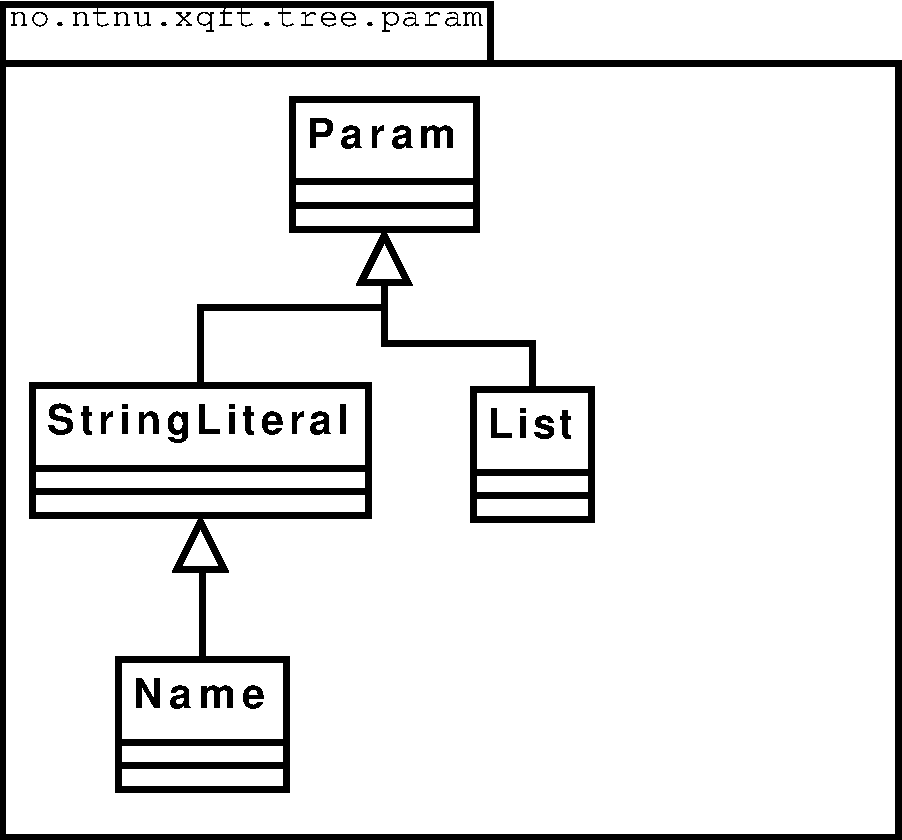
\includegraphics[scale=0.5]{diagrams/mql_param_uml}
  \caption{Class diagram of MQL parameters}
  \label{fig:impl:mql_param_uml}
\end{center}
\end{figure}

MQL parameters (as described in \ref{sect:method:mql:concepts}) are modeled as
seen in figure \ref{fig:impl:mql_param_uml}. Parameters require no complex
structure, and are only created and added to operators as needed.

\subsection{Concepts}
As mentioned, MQL queries are represented as trees, where each node represents
an operator. Each node is an instance of an operator class (as described
above), and contains a list of child operators and a list of parameters. To
convert the operator tree to a MQL query string, simply call the method
\texttt{toPrettyString(0)} on the root node of the operator tree.

\subsection{Usage}
The operator classes are designed to be intuitive and simple to use. Figure
\ref{fig:impl:mql_op_ex1_java} shows one example where a simple operator tree
is built and converted to an MQL query string (the result of which can be seen
in figure \ref{fig:impl:mql_op_ex1_mql}).

%\usepackage{graphics} is needed for \includegraphics
\begin{figure}[htp]
\begin{center}
  \begin{Verbatim}
Lookup lookup = new Lookup("Death in the clouds");
Scope scope = new Scope("/books/book/title", lookup);
Project project = new Project("author", scope);
System.out.println(project.toPrettyString(0));
  \end{Verbatim}
  \caption{Example java code to construct a MQL operator tree}
  \label{fig:impl:mql_op_ex1_java}
\end{center}
\end{figure}

\begin{figure}[htp]
\begin{center}
  \begin{Verbatim}
project([author];
  scope(/books/book/title;
    lookup("Death in the clouds")))
  \end{Verbatim}
  \caption{Resulting MQL query string from example in figure
  \ref{fig:impl:mql_op_ex1_java}}
  \label{fig:impl:mql_op_ex1_mql}
\end{center}
\end{figure}

\section{Context-sensitive visitor}
\label{sect:impl:context_sens_visitor}
In section \ref{sect:theory:parser:tree_parsing} a number of techniques for
tree parsing were presented. In section \ref{sect:method:tree_parsing} the
\textit{context-sensitive visitor pattern} was chosen as the technique for this
implementation. This section will detail the implementation of this design
pattern, and how it is used to performed an assortment of tasks.

\subsection{Basics}
The context-sensitive pattern is designed to be flexible and to generate code
with a higher level of maintainability, for which the rationale was presented
in section \ref{sect:theory:contextVisitorPattern}. 

\begin{figure}[htp]
\begin{center}
  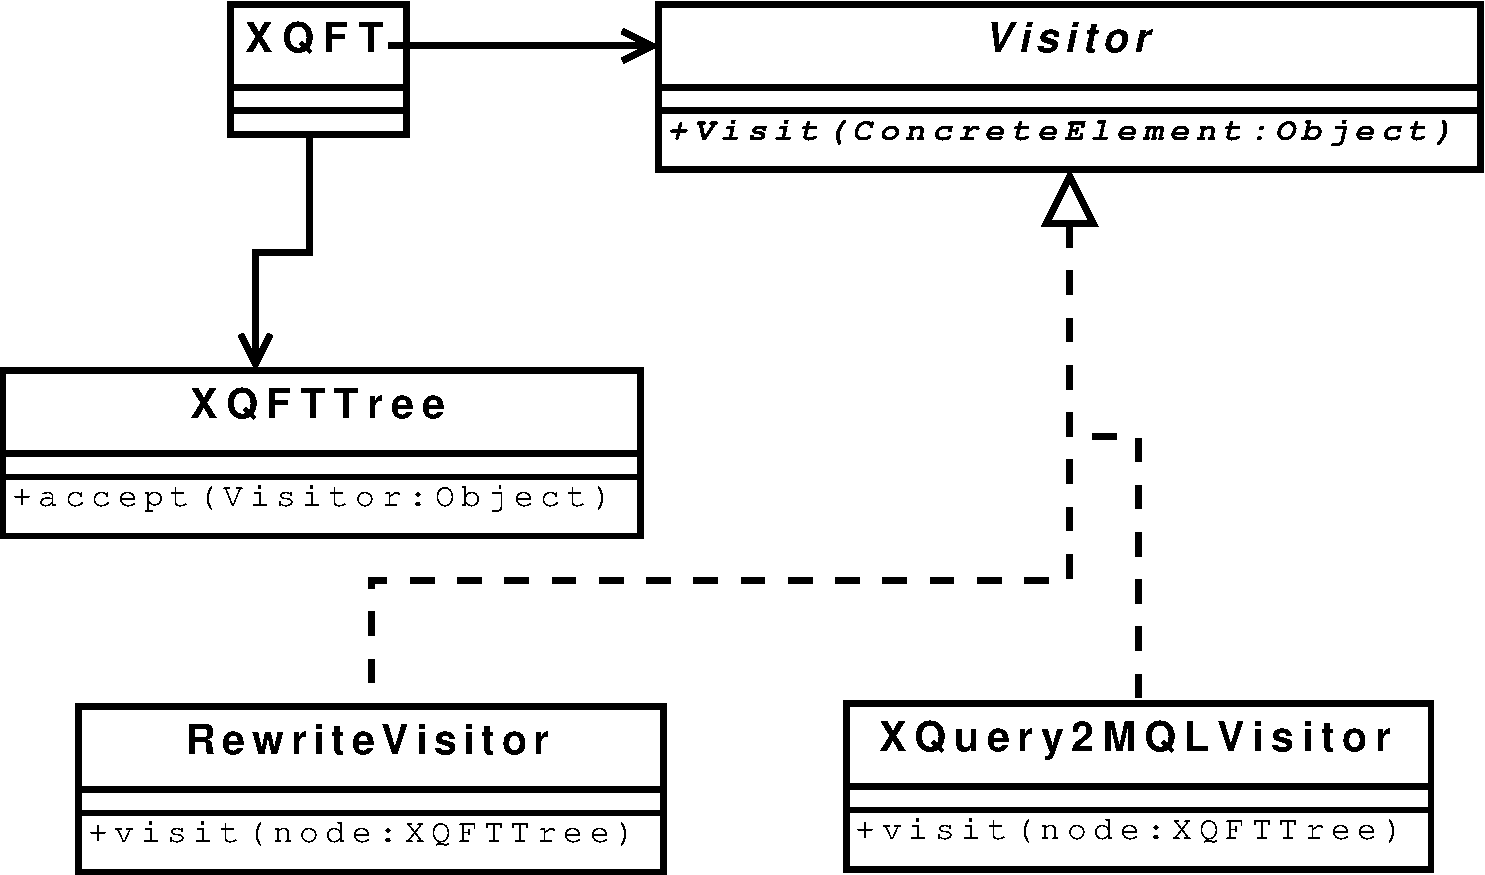
\includegraphics[scale=0.5]{diagrams/context_visitor_pattern_impl}
  \caption{Context sensitive visitor implementation}
  \label{fig:impl:context_sens_visitor_impl}
\end{center}
\end{figure}

The class diagram for the actual implementation of the context-sensitive
visitor pattern can be seen in figure \ref{fig:impl:context_sens_visitor_impl}.
Compare this to the generalized class diagram in figure
\ref{figure:parser:context_visitor_pattern} on page
\pageref{figure:parser:context_visitor_pattern}.

Note that the use of \texttt{XQFTTree} as the element class implies that the
\texttt{XQFTTree} be supplemented with an \texttt{accept()} method to
accommodate this pattern. This method is essentially a static dispatcher which
will call the appropriate method on the visitor based on the token type of the
node currently being visited. Figure \ref{} shows an excerpt of this method and
how it acts on the visitor class.

%\usepackage{graphics} is needed for \includegraphics
\begin{figure}[htp]
\begin{center}
  \begin{Verbatim}	
public TraverseReturn accept(Visitor visitor) {
     case XQFTParser.AST_MODULE:
            return visitor.visitAST_MODULE(this);
        case XQFTParser.AST_FLWOR:
            return visitor.visitAST_FLWOR(this);
        case XQFTParser.AST_FORCLAUSE:
            return visitor.visitAST_FORCLAUSE(this);
        case XQFTParser.AST_LETCLAUSE:
            return visitor.visitAST_LETCLAUSE(this);
        case XQFTParser.AST_ORDERBYCLAUSE:
            return visitor.visitAST_ORDERBYCLAUSE(this);
        case XQFTParser.AST_WHERECLAUSE:
            return visitor.visitAST_WHERECLAUSE(this);
                          .
                          .
                          .
  \end{Verbatim}
  \caption{Excerpt from the accept() method in the XQFT class}
  \label{figureLabel}
\end{center}
\end{figure}

\subsection{The Rewrite visitor}
The \textit{Rewrite visitor} is used to perform rewrite operations on the
abstract syntax tree before performing the actual translation. In particular,
these rewrite operations consists of normalizing the required subtrees of the
syntax tree to a subset of XQuery Core (as described in sections
\ref{sect:theory:xquery:XQcore} and \ref{sect:method:ast_rewrite}).

\subsection{The XQuery2MQL visitor}
The \textit{XQuery2MQL visitor} performs the bulk of the work related to
performing the translation of XQuery to MQL. This visitor is capable of
re-instantiating itself (or other visitors) when entering new contexts, such as
path predicates. 
\section{Scoping and Symbol Tables}
Crucial to the implementation of the Tainting Dependencies (TD) methodology
described in chapter \ref{chapter:translation} is the ability to
maintain a contextual environment with scoping and symbol tables. This section
details the implementation of this, and how it is used to meet the
requirements of TD.

\subsection{Concepts}
The scoping system in the implementation is based on building a scope tree. The
previous scope, if any, is set as parent of the new scope, and the previous
scope maintains a list of child scopes -- this is referred to as
\textit{pushing a scope}. When exiting a scoped subexpression in the AST, the
previous scope is again set as the current scope. This is referred to as
\textit{popping a scope}. A reference to the root scope node is always
maintained. Considering the example XQuery query in figure
\ref{fig:impl:scope_tree_ex_code}, the scope tree in figure
\ref{fig:impl:scope_tree_ex} is generated. The scope itself contains \emph{one}
symbol table for the current scope.

\begin{figure}[!htp]
\begin{center}
\begin{minipage}[h]{9cm}
\begin{verbatim}
for $i in (1,2,3) return 
  for $a in (4,5,for $b in (6,7,8) return $b) 
    return ($i,$a)
\end{verbatim}
  \caption{Scope tree example code}
  \label{fig:impl:scope_tree_ex_code}
  \end{minipage}
\end{center}
\end{figure}

\begin{figure}[!htp]
\begin{center}
  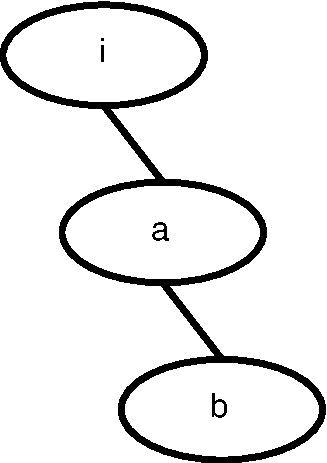
\includegraphics[width=0.2\textwidth]{diagrams/scope_tree_ex}
  \caption{Scope tree for source code in figure
  \ref{fig:impl:scope_tree_ex_code}} 
  \label{fig:impl:scope_tree_ex}
\end{center}
\end{figure}

Entries in the symbol table are represented through an instance of the
\texttt{SymTabEntry} class which maintains metadata about symbols (such as
symbol name, a flag indicating whether it's an iterator variable, and an
evaluated expression). The symbol table is realised as a subclass of the
\texttt{HashMap} class in the \texttt{java.util} package, and is constrained to
storing instances of \texttt{SymTabEntry}, with the symbol name as key.

\subsection{Semantics}
The scoping semantics are encapsulated in a singleton manner in the class
\texttt{Scope}, with static methods available for pushing and popping scopes,
and storing and retrieving symbols. The external (static) API as available to a
user of the scope system is shown in figure \ref{fig:impl:scope_uml}.

\begin{figure}[!htp]
\begin{center}
  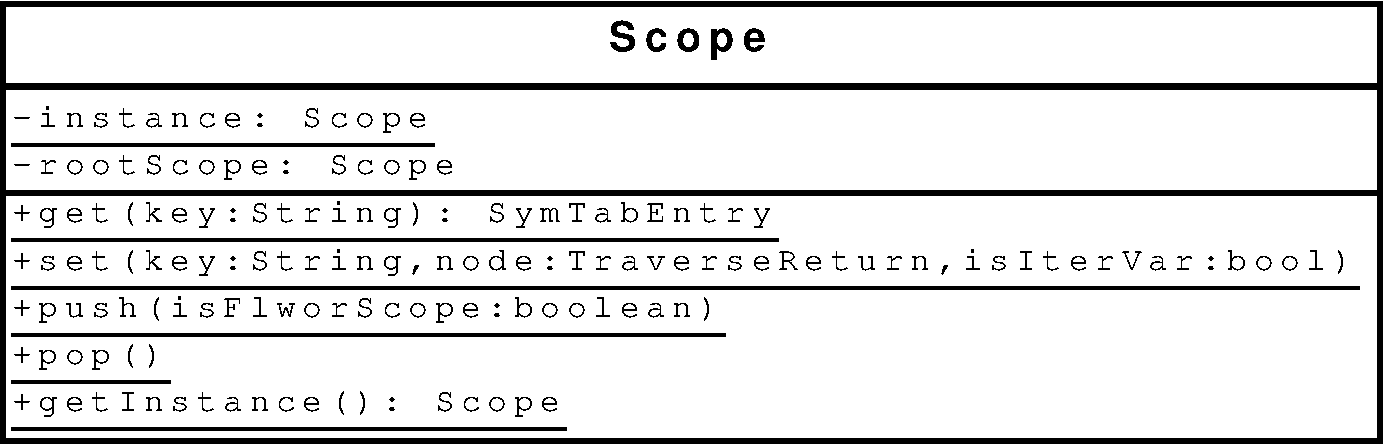
\includegraphics[width=0.7\textwidth]{diagrams/scope_uml}
  \caption{Scope API}
  \label{fig:impl:scope_uml}
\end{center}
\end{figure}

A new scope is \textit{pushed} whenever a \texttt{for}-clause is encountered while
parsing the abstract syntax tree, and the current scope is \textit{popped} after
evaluating a \texttt{return}-clause -- both of which occur within a FLWOR expression.

The scoping system also tracks iteration variables. That is, for any scope,
there is \textit{one and only one} iteration variable, except in the top scope
where there is no iteration variable. The concept of an iteration variable is
explained in definition \ref{def:iterVarDep}. Tracking of these
variables are reviewed in section \ref{sect:impl:tainting_deps}.
\section{Passing Metadata Between Nodes}
To implement the Tainting Dependencies method it is necessary to pass
metadata upwards when parsing the syntax tree, such as
iterator dependencies and flags to indicate singleton nodes (for simplifications). Additionally, the
operator tree which is being built bottom-up (as described earlier in section
\ref{sect:impl:construct_mql}) is also required to be passed upwards. 

This is achieved through the \texttt{TaverseReturn}, which models a return type
when visiting nodes in the syntax tree. That is, the visitor methods are
responsible of 1) visiting any child nodes, and 2) returning an instance of the
\texttt{TraverseReturn} class based on what was returned from the child nodes,
if anything.

\subsection{The TraverseReturn Class}
The class diagram for the \texttt{TraverseReturn} class is shown in figure
\ref{fig:impl:meta:traverse_uml}. Note the flag to indicate if the current
context is a singleton, the reference to an MQL operator tree (which is being
built bottom-up), and a reference to a set of iterator dependencies (in the implementation called
\texttt{varRefs}).

\begin{figure}[!htp]
\begin{center}
  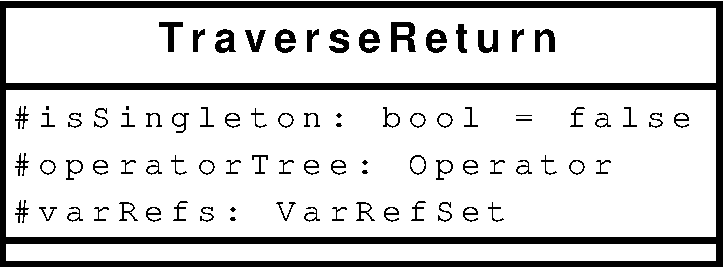
\includegraphics[scale=0.5]{diagrams/traversereturn_uml}
  \caption{TraverseReturn class diagram}
  \label{fig:impl:meta:traverse_uml}
\end{center}
\end{figure}

The \texttt{TraverseReturn} class is, as mentioned, used in the visitor when
visiting nodes in the abstract syntax tree (see section
\ref{sect:impl:context_sens_visitor}). A typical use case is shown in figure
\ref{fig:impl:meta:traverse_usage_ex}, which is an excerpt from the
implementation.

\subsection{Iterator Dependencies}
Iterator dependencies, described in section \ref{sect:trans:TD:basics}, are
passed upwards together with the MQL operator tree being built during the syntax
tree parsing process. These sets of dependencies are handled by th \texttt{VarRef} and \texttt{VarRefSet} classes.
A class diagram for these classes is shown in figure \ref{fig:impl:meta:varrefset_uml}.

\begin{figure}[!htp]
\begin{center}
  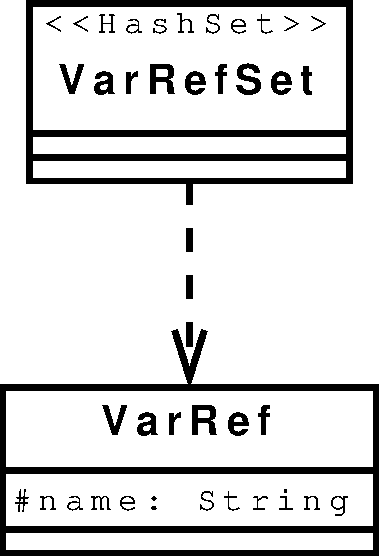
\includegraphics[scale=0.5]{diagrams/varrefset_uml}
  \caption{\texttt{VarRefSet} and \texttt{VarRef} class diagram}
  \label{fig:impl:meta:varrefset_uml}
\end{center}
\end{figure}

As described in section \ref{sect:trans:TD:dependency}, an iterator variable reference is always dependent on
its corresponding iterator. Thus, when a iterator variable is encountered during the parse process, and the
variable is being ``read'' and not assigned or declared, the corresponding iterator is added to the current set of
iterator dependencies. The example in figure \ref{fig:impl:meta:var_ref_ex} shows the variable \texttt{\$a}
being read, in which case the iterator is added to the \texttt{TraverseReturn}
to-be-returned's set of dependencies.

\begin{figure}[!htp]
\begin{center}
\begin{minipage}[h]{5cm}
\begin{verbatim}
for $i in (1,2,3) return 
    ($a,4,5)
\end{verbatim}
\end{minipage}
  \caption{Example of the variable \texttt{\$a} being read. Note that the iterator
  variable \texttt{\$i} is never read}
  \label{fig:impl:meta:var_ref_ex}
\end{center}
\end{figure}

The source code excerpt in figure \ref{fig:impl:meta:var_ref_impl2} shows how
iterator dependencies are treated in the visitor implementation.

\begin{figure}[!htp]
\begin{center}
\begin{Verbatim}
// Fetch entry from symtab
SymTabEntry entry = Scope.get(tree.getChild(0).getText());
            
// Obtain and append new var ref
TraverseReturn tr = entry.getTraverseReturn();
tr.getVarRefs().add(new VarRef(tree.getChild(0).getText()));

return tr;
\end{Verbatim}
  \caption{Appending a new variable reference}
  \label{fig:impl:meta:var_ref_impl2}
\end{center}
\end{figure}

\subsection{Singleton nodes}
Singleton nodes are nodes corresponding to expressions that return a sequence of exactly one item. In
the cases where this is known to be true, the result from a translation can be
tagged with this information and used later to simplify the translation of
sequence construction (as described in section \ref{sect:impl:td:seq}).

This is the case of integer literal nodes as well as iterator variable lookups in the
symbol table. The case of integer literal nodes is shown in figure
\ref{fig:impl:meta:traverse_usage_ex} in the next section. The case of variable
lookups is somewhat less intuitive, since the singleton flag is actually
stored when a variable is first set. That is, the right-hand side of the
assignment is translated once and annotated with the singleton flag, which is
then set for all subsequent lookups in the symbol table. The excerpt in figure 
\ref{fig:impl:meta:var_assign_ex} shows how this is done in the implementation.

\begin{figure}[!htp]
\begin{center}
\begin{Verbatim}
// Visit children on the right side of the assignment
TraverseReturn tr = acceptThis(tree.getChild(1));

// Required for tainting deps method
Project project = new Project("[" + varName + "numb, value]", 
                      tr.getOperatorTree());

// Assign metadata
tr.setOperatorTree(project);
tr.setSingleton(true);

// Enter into symbol table
SymTabEntry tmp = Scope.set(tree.getChild(0).getText(), 
                      tr, isIterationVar);
\end{Verbatim}
  \caption[Iterator variable annontion with singleton flag]{Iterator variable
  assignment example, annotated with the singleton flag before being entered into the symtab}
  \label{fig:impl:meta:var_assign_ex}
\end{center}
\end{figure}

\subsection{Example of usage}
In the example in figure \ref{fig:impl:meta:traverse_usage_ex}, an
integer literal node is visited (a node that simply holds an integer). A
\texttt{make()} MQL operator as well as a new \texttt{TraverseReturn}
instance is created. The \texttt{make()} operator is then appended to the 
\texttt{TraverseReturn} instance, and the \textit{isSingleton} flag is set to 
\textit{true} since the result of this translation is a single item.

\begin{figure}[!htp]
\begin{center}
\begin{Verbatim}
public TraverseReturn visitIntegerLiteral(XQFTTree tree) {

    Make make = new Make("name:=[index, value], [1, " + tree.getText());
    TraverseReturn tr = new TraverseReturn();        
    tr.setSingleton(true);
    tr.setOperatorTree(make);
    return tr;
}
\end{Verbatim}
  \caption{TraverseReturn usage example}
  \label{fig:impl:meta:traverse_usage_ex}
\end{center}
\end{figure}
\section{Tainting dependencies}
``Tainting dependencies'' is a method of translating XQuery queries to
relational algebra. The semantics of this method is described in detail
throughout section \ref{sect:trans:taintingDependencies}. This section
describes an implementation of a subset of this method which is capable of
translating simple FLWOR expressions, sequences, and variables. 

\label{sect:impl:tainting_deps}
Dette blir den lengste seksjonen i dette kapittelet, h\aa per jeg.
\subsection{FLWOR expressions}



\subsection{Sequences}
\label{sect:impl:td:seq}
\begin{itemize}
  \item behandler parantes istf. komma for sekvenser (ref spec) 
\end{itemize}

\section{Summary}
\label{sect:impl:summary}
This chapter has described the implementation of a proof of concept for the
``Tainting Dependencies'' method. In the next chapter, some results are
presented, such as theoretical algebra output. Additionally, algebra generated
by the prototype described here will be compared to that generated by
Pathfinder.

%RESULTS
\chapter{Results}
\label{chapter:results}
This chapter will showcase a series of relational algebra trees. First, in
section \ref{sect:result:theoretical_algebra}, example trees computed by hand
using the rules for ``Tainting Dependencies'' are presented, showcasing
some major capabilities of this method. Further, in section
\ref{sect:result:implementation_algebra}, some trivial and complex queries are
generated by the prototype implementation and displayed. Furthermore, in
section \ref{sect:results:comparison}, comparisons are made to algebra
generated by Pathfinder/MonetDB using classic loop lifting.

\section{Theoretical Algebra}
\label{sect:result:theoretical_algebra}
In this section, a collection of XQuery query examples and their translation to
relational algebra is presented. The translation is done manually using the
``Tainting Dependencies'' method described in chapter \ref{sect:translation}. For the sake of
brevity, only the rules used throughout the translation will be noted. Intermediate results will
not be included.

Generell struktur:
- Sp\oe rring
- Semantikk (resultat)
- Translasjon
- Mellomregninger? (naaii..)

\subsection{Extensive FLWOR}
This example will illustrate the translation of a more complex FLWOR expression.

\subsubsection{Query premise}
\begin{figure}[!htp]
\begin{center}
\begin{Verbatim}
for $a in (1,2,3) let $b := 2
  where $a gt $b
  order by $a
  return ($a, $b)
\end{Verbatim}
  \caption{Extensive FLWOR expression, showcasing for-, let-, where-, orderby-,
  and return-clauses}
  \label{fig:results:query_ext_flwor}
\end{center}
\end{figure}

\subsubsection{Translation process}
The translation process in its entirety is shown step by step in appendix
\ref{appendix:transl:ext_flwor}, page \pageref{appendix:transl:ext_flwor}.

\subsubsection{Result}
The result of the translation is shown in figure
\ref{fig:results:query_ext_flwor_result}.

\begin{figure}[!htp]
\begin{center}
  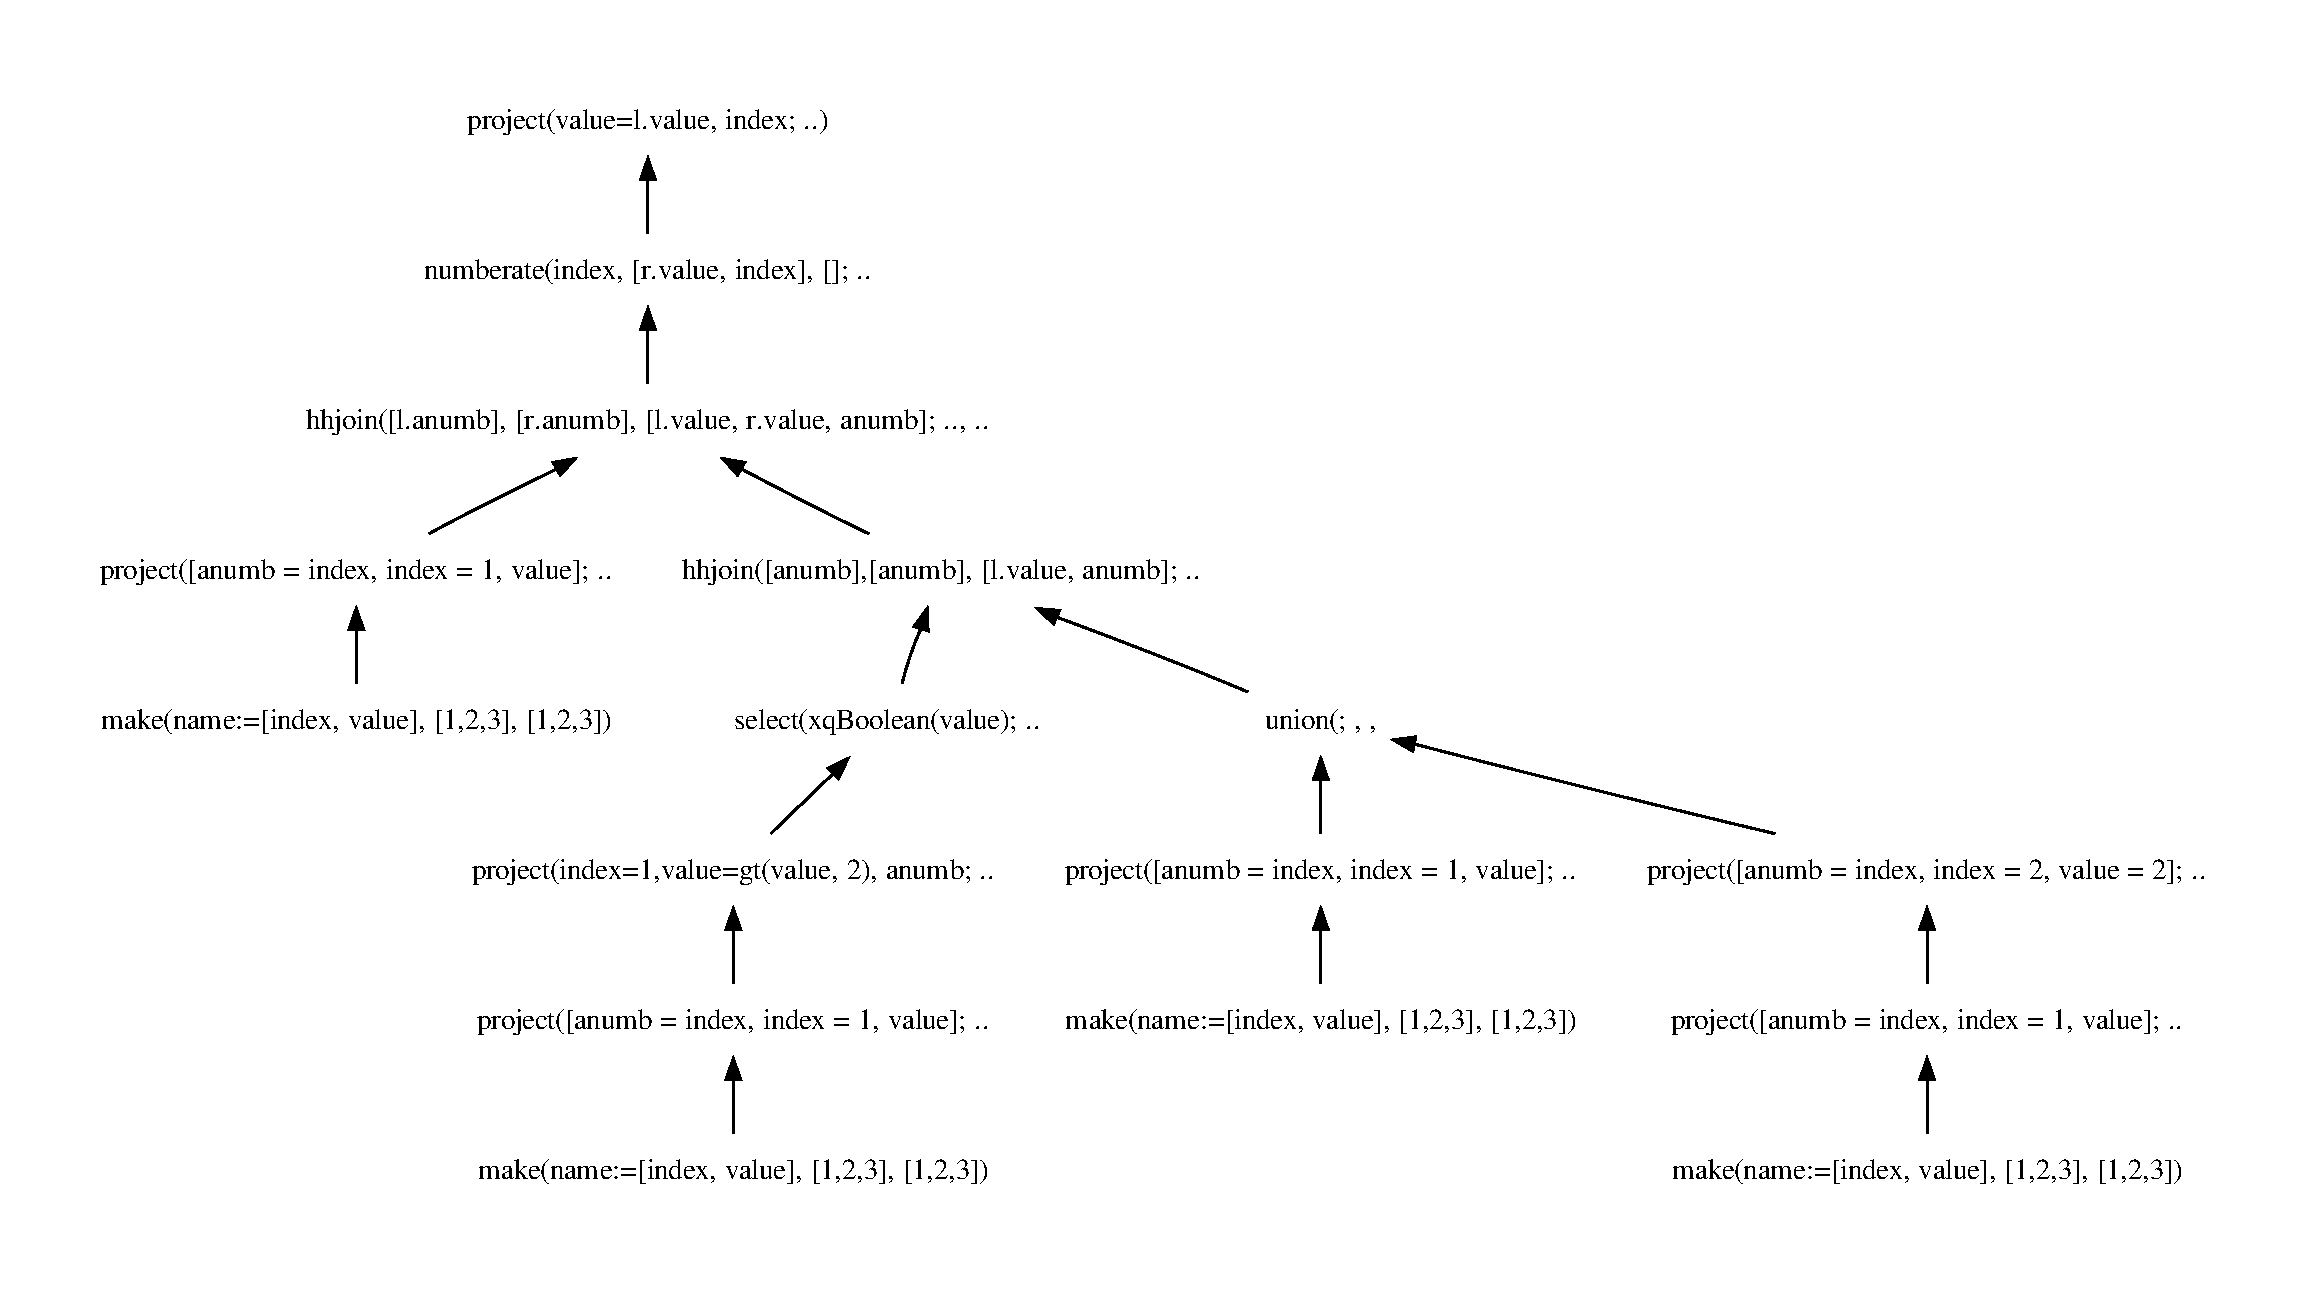
\includegraphics[width=1.0\textwidth]{img/graphs/ext_flwor}
  \caption{Complete translation of expression in figure
  \ref{fig:results:query_ext_flwor}}
  \label{fig:results:query_ext_flwor_result}
\end{center}
\end{figure}

The operator tree in figure \ref{fig:results:query_ext_flwor_result} can be
converted to the DAG seen in figure \ref{fig:results:query_ext_flwor_dag}.

\newpage

\begin{figure}[!htp]
\begin{center}
  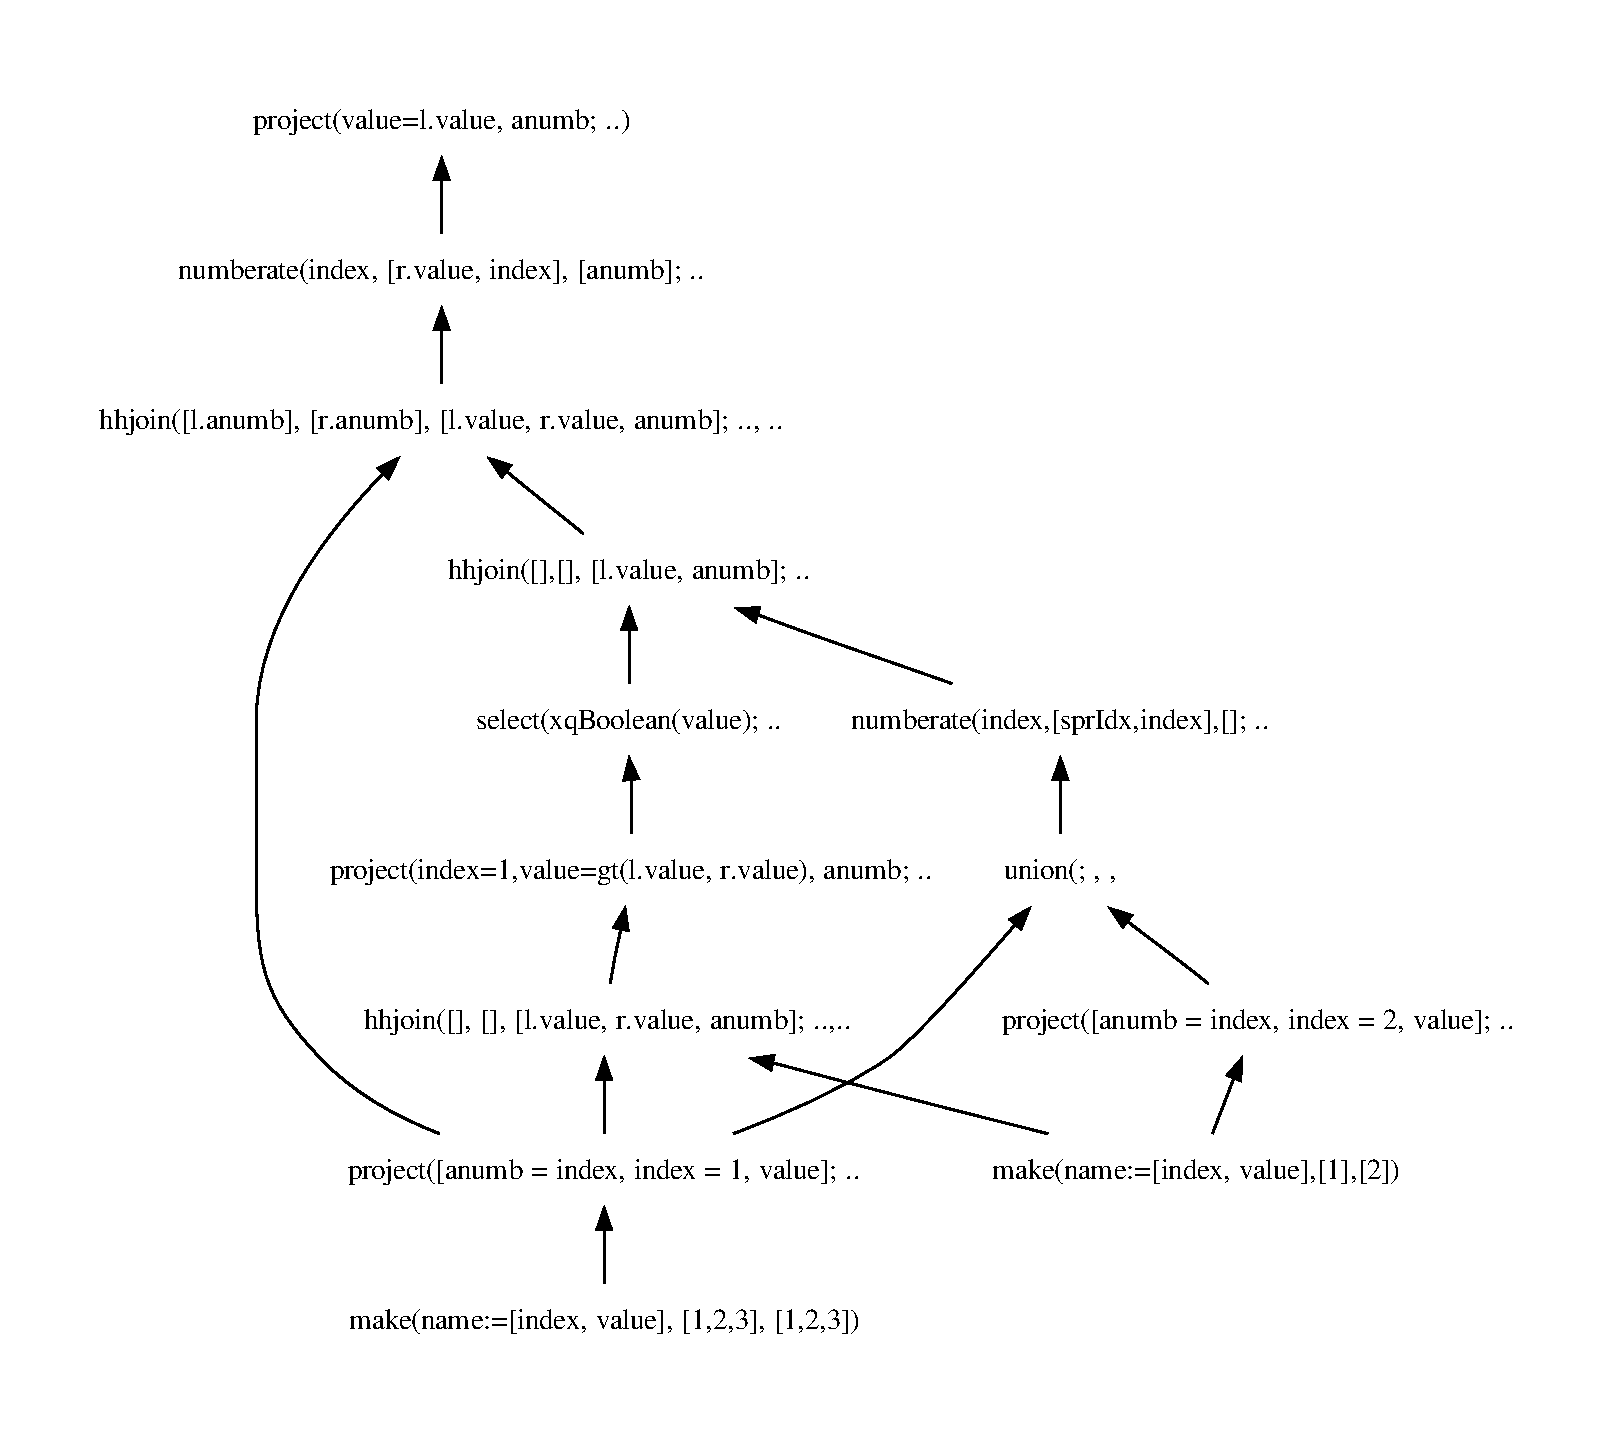
\includegraphics[width=1.0\textwidth]{img/graphs/ext_flwor_dag}
  \caption{DAG representation of operator tree in figure
  \ref{fig:results:query_ext_flwor_result}}
  \label{fig:results:query_ext_flwor_dag}
\end{center}
\end{figure}

\subsection{Path expression with predicate}
This example will illustrate the translation of a path expression with a predicate.

\subsubsection{Query premise}
\begin{figure}[!htp]
\begin{center}
\begin{Verbatim}
/a/b[@id eq 2] 
\end{Verbatim}
  \caption{Path expression with a predicate query premise}
  \label{fig:results:query_pathPred}
\end{center}
\end{figure}

\subsubsection{Translation process}
The translation process in its entirety is shown step by step in appendix
\ref{appendix:transl:pathPred}, page \pageref{appendix:transl:pathPred}.

\subsubsection{Result}
The result of the translation is shown in figure
\ref{fig:results:query_pathpred_result}.

\begin{figure}[!htp]
\begin{center}
  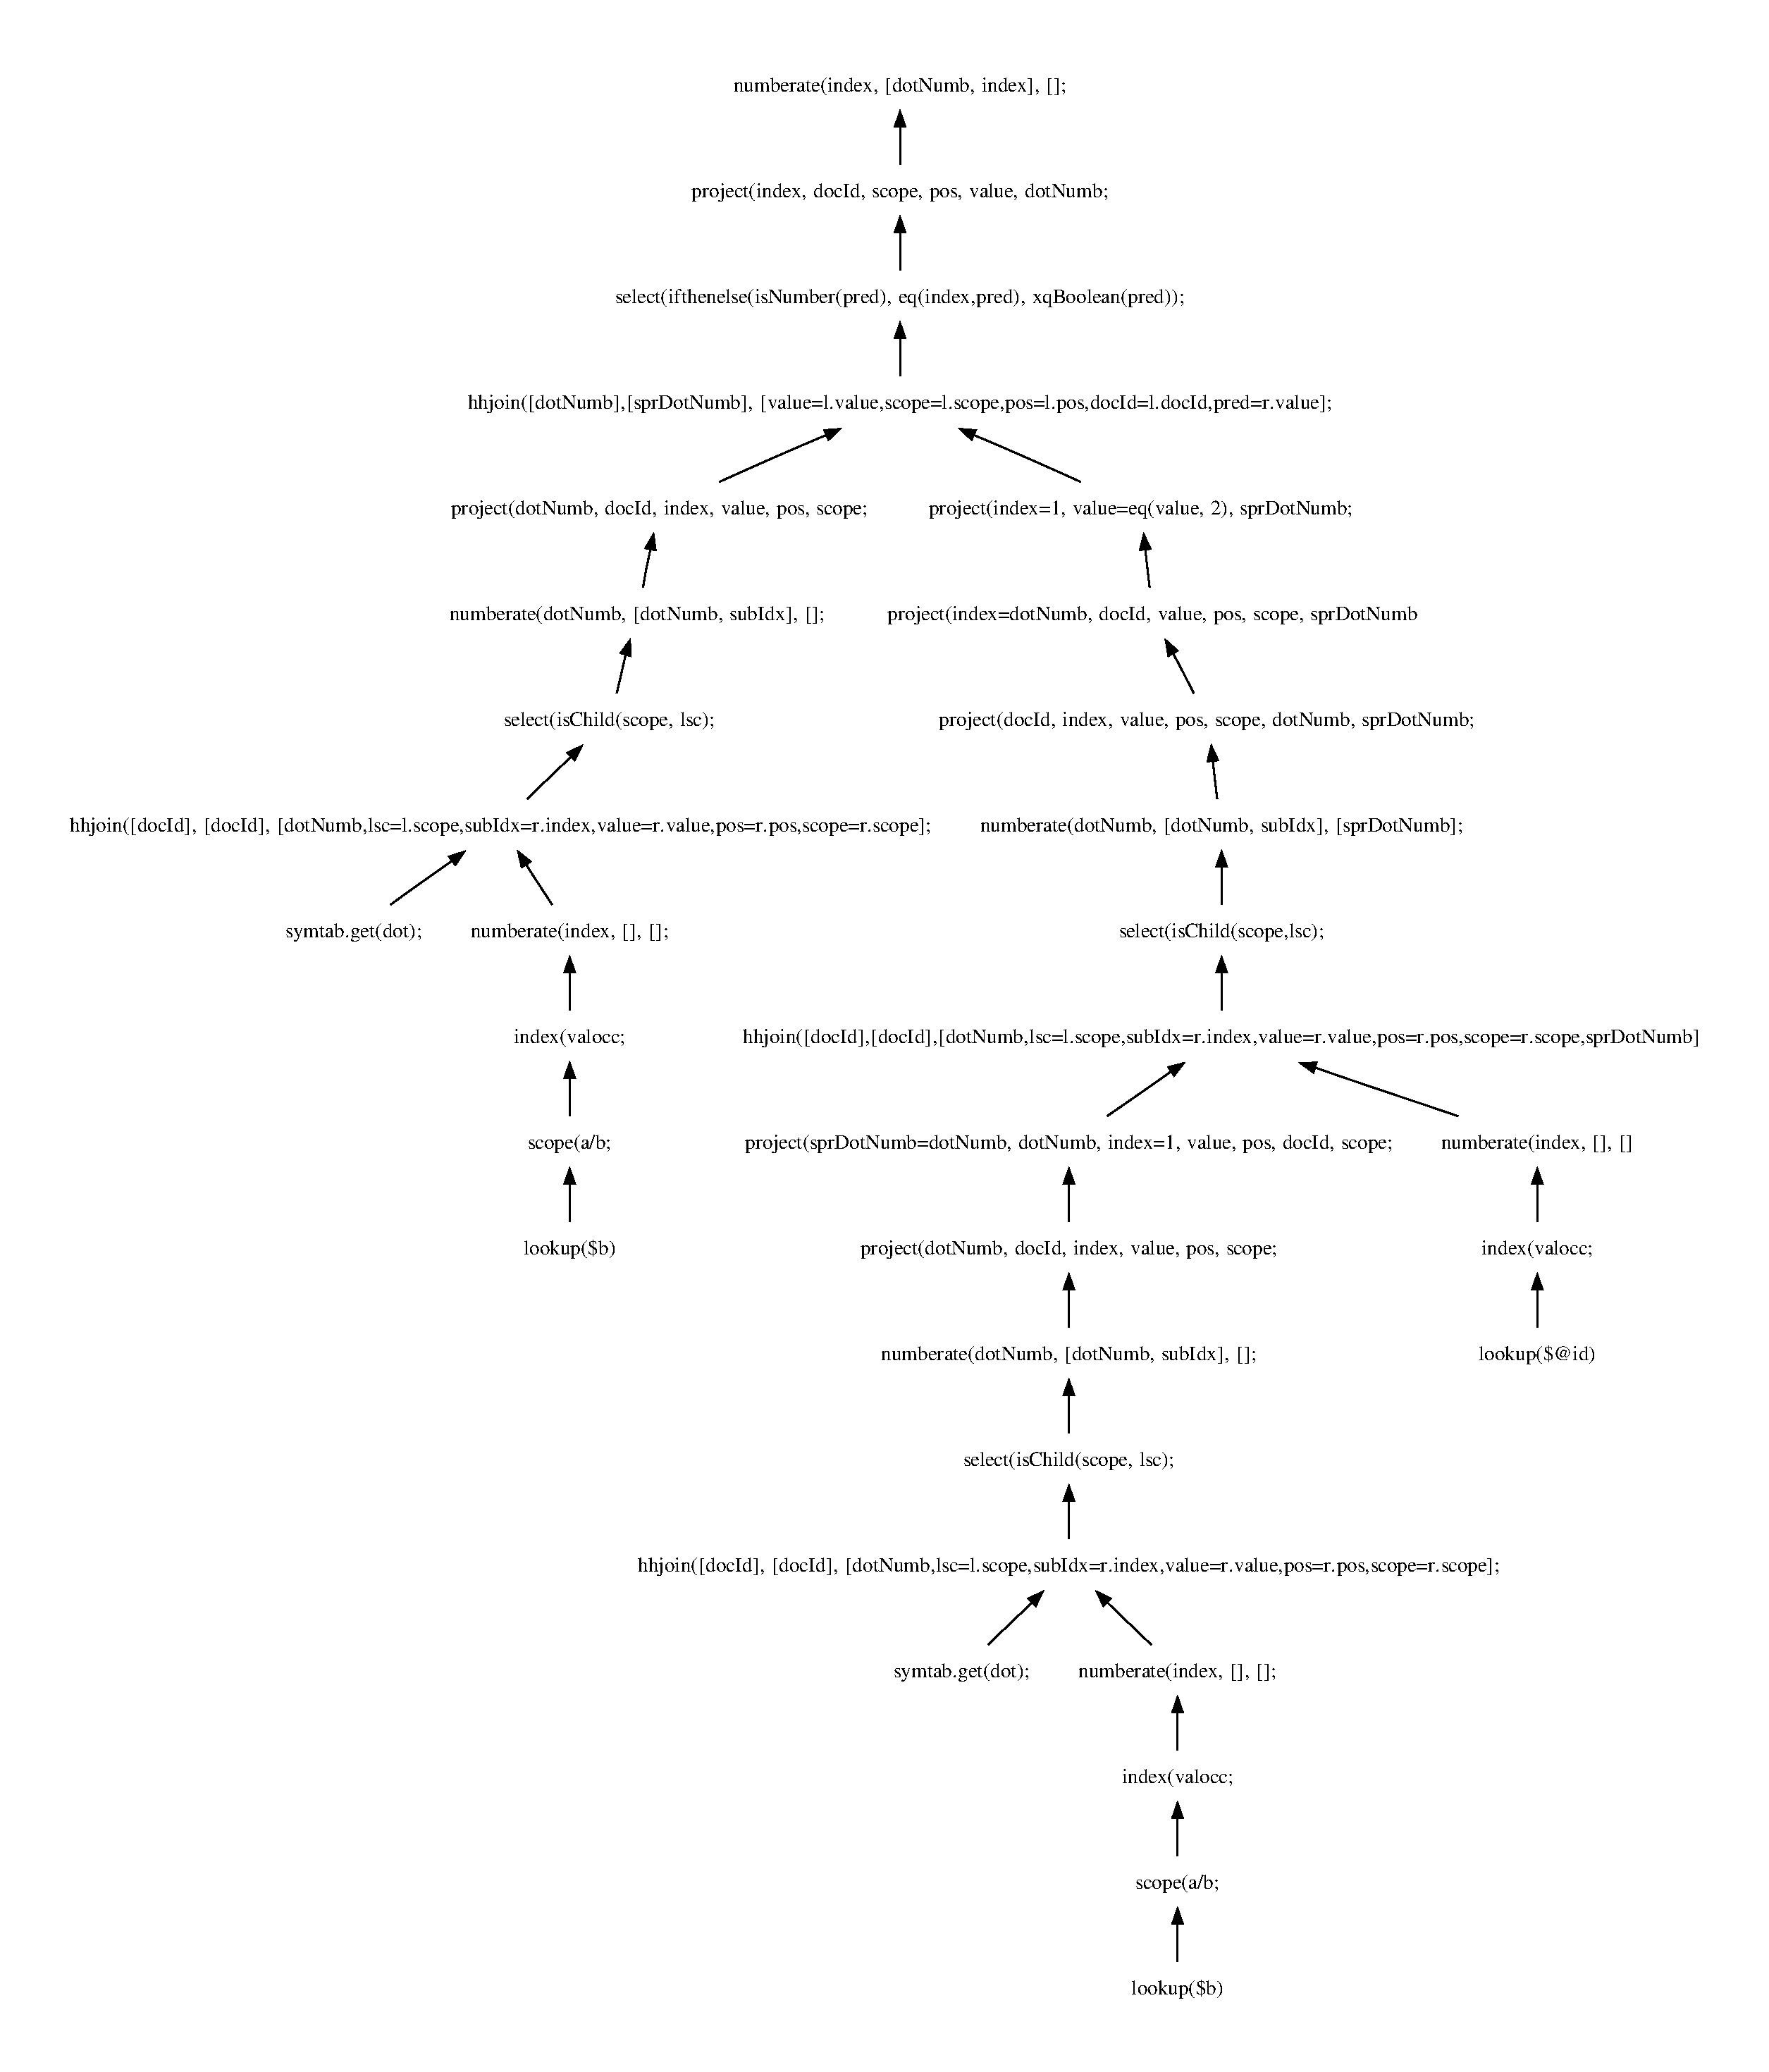
\includegraphics[width=1.0\textwidth]{img/graphs/TD_patExprPred}
  \caption{Complete translation of expression in figure
  \ref{fig:results:query_pathPred}}
  \label{fig:results:query_pathpred_result}
\end{center}
\end{figure}

The operator tree in figure \ref{fig:results:query_pathpred_result} can be
converted to the DAG seen in figure \ref{fig:results:query_pathpred_result_dag}.

\newpage

\begin{figure}[!htp]
\begin{center}
  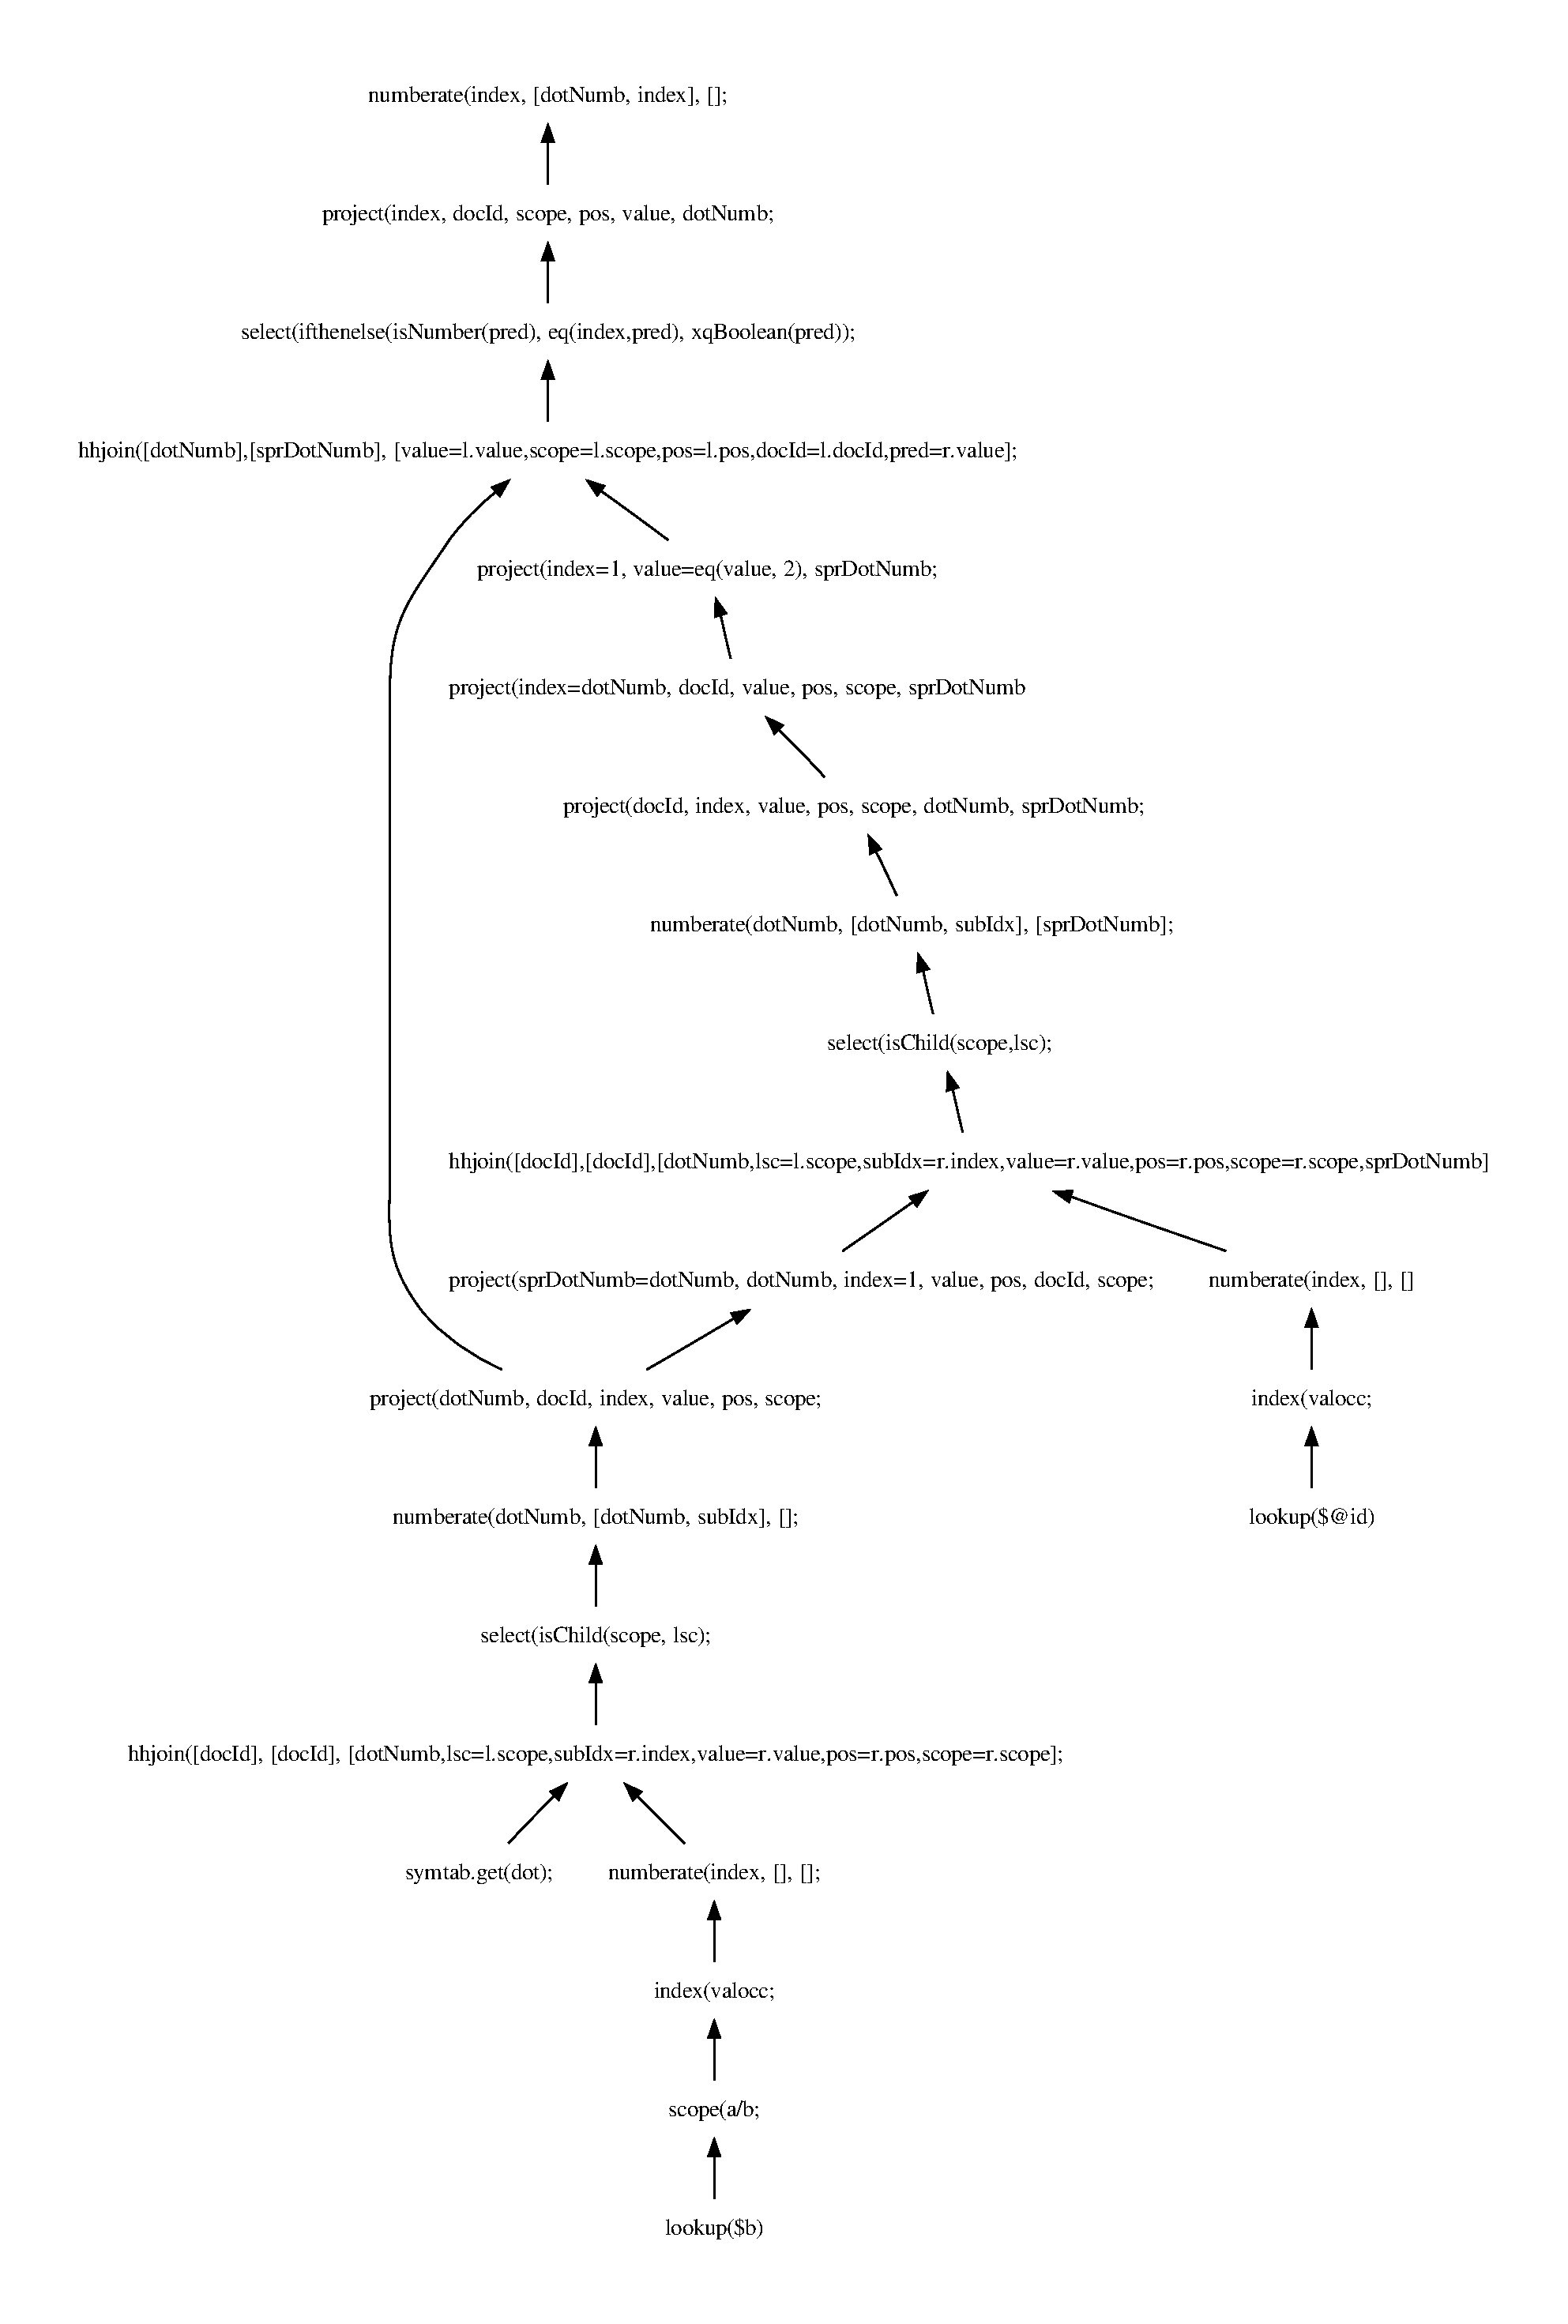
\includegraphics[width=1.0\textwidth]{img/graphs/TD_patExprPred_dag}
  \caption{DAG representation of operator tree in figure
  \ref{fig:results:query_pathpred_result}}
  \label{fig:results:query_pathpred_result_dag}
\end{center}
\end{figure}

\subsection{If-then-else}
\subsubsection{Query premise}
\begin{figure}[!htp]
\begin{center}
\begin{Verbatim}
for $a in (1,2,3) return
  if $a gt 2 then $a else 3
\end{Verbatim}
  \caption{If-then-else query premise}
  \label{fig:results:query_ifthenelse}
\end{center}
\end{figure}

\subsubsection{Translation process}
The translation process in its entirety is shown step by step in appendix
\ref{appendix:transl:ifthenelse}, page \pageref{appendix:transl:ifthenelse}.

\subsubsection{Result}
The result of the translation is shown in figure
\ref{fig:results:query_ifthenelse_result}.

\begin{figure}[!htp]
\begin{center}
  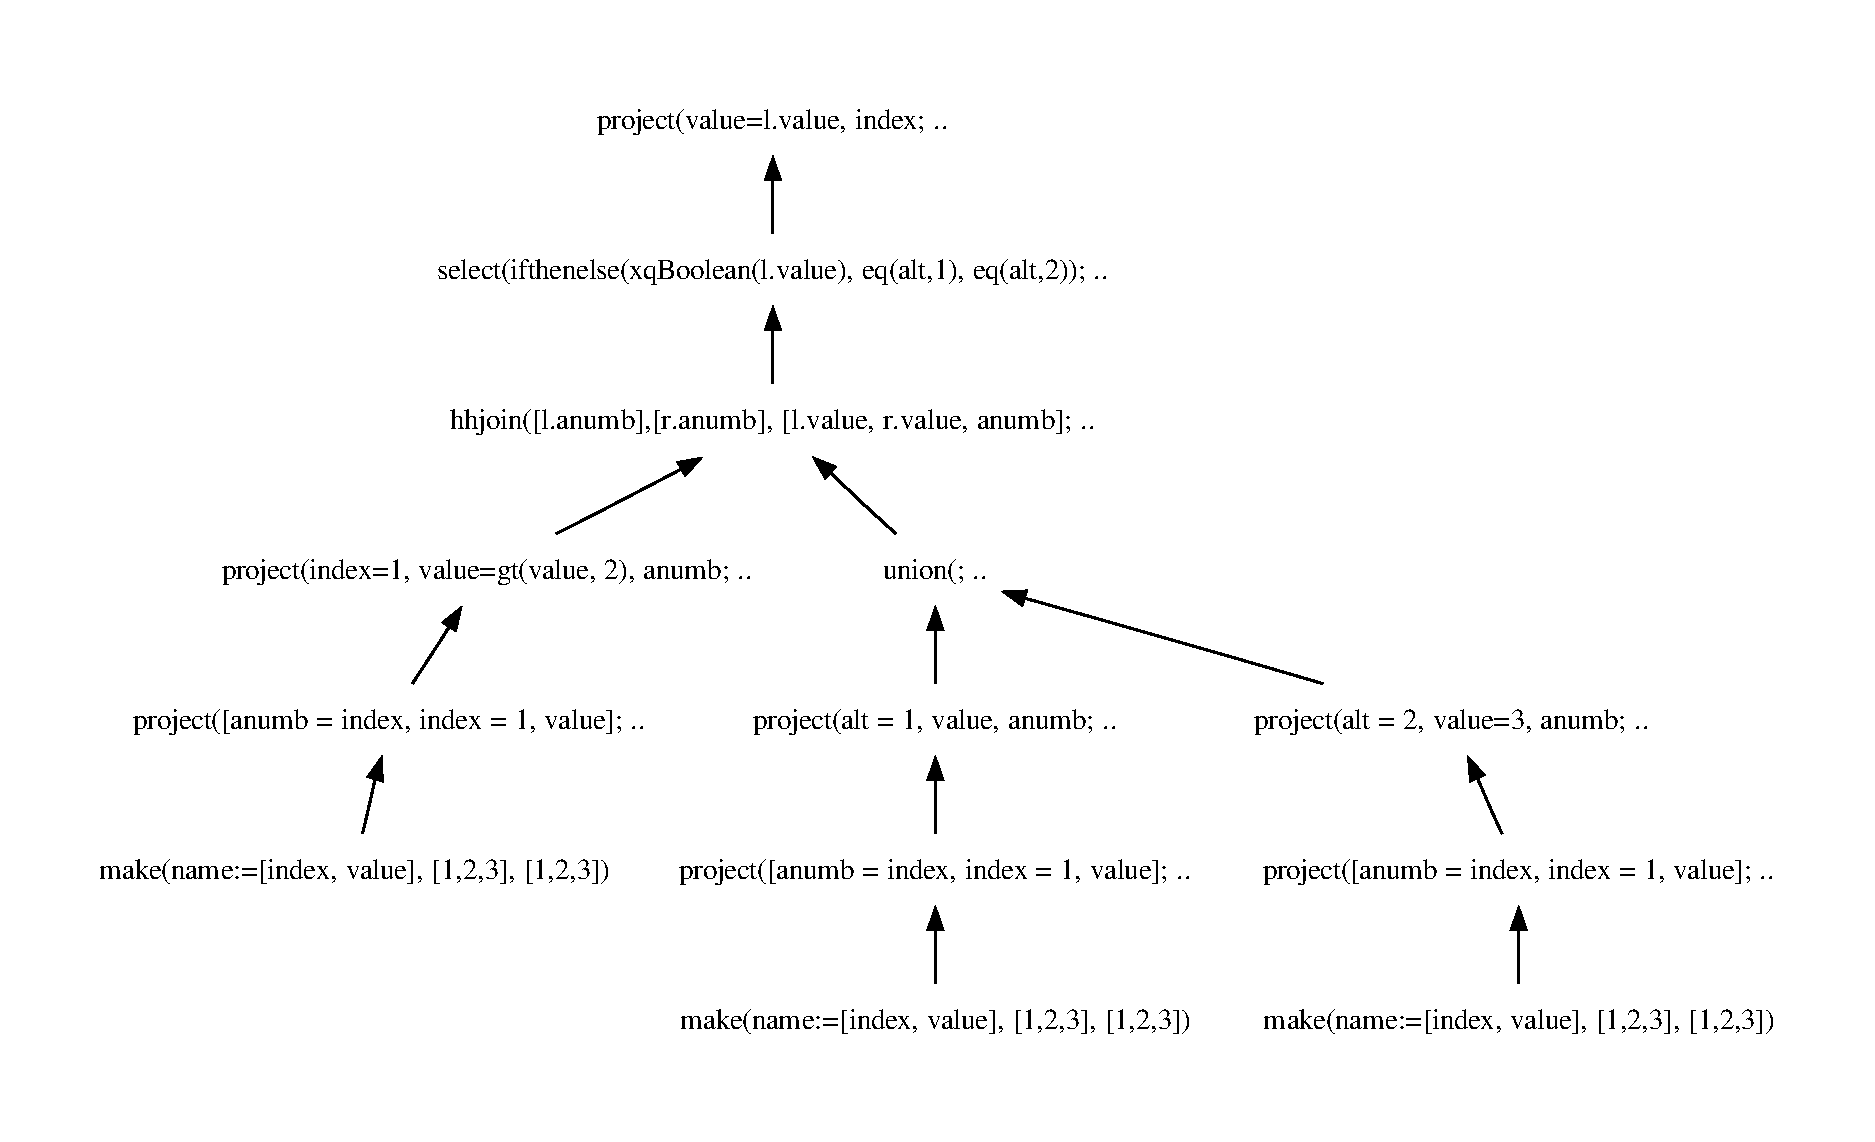
\includegraphics[width=1.0\textwidth]{img/graphs/ifthenelse}
  \caption{Complete translation of expression in figure
  \ref{fig:results:query_ifthenelse}}
  \label{fig:results:query_ifthenelse_result}
\end{center}
\end{figure}

The operator tree in figure \ref{fig:results:query_ifthenelse_result} can be
converted to the DAG seen in figure \ref{fig:results:query_ifthenelse_result_dag}.

\newpage

\begin{figure}[!htp]
\begin{center}
  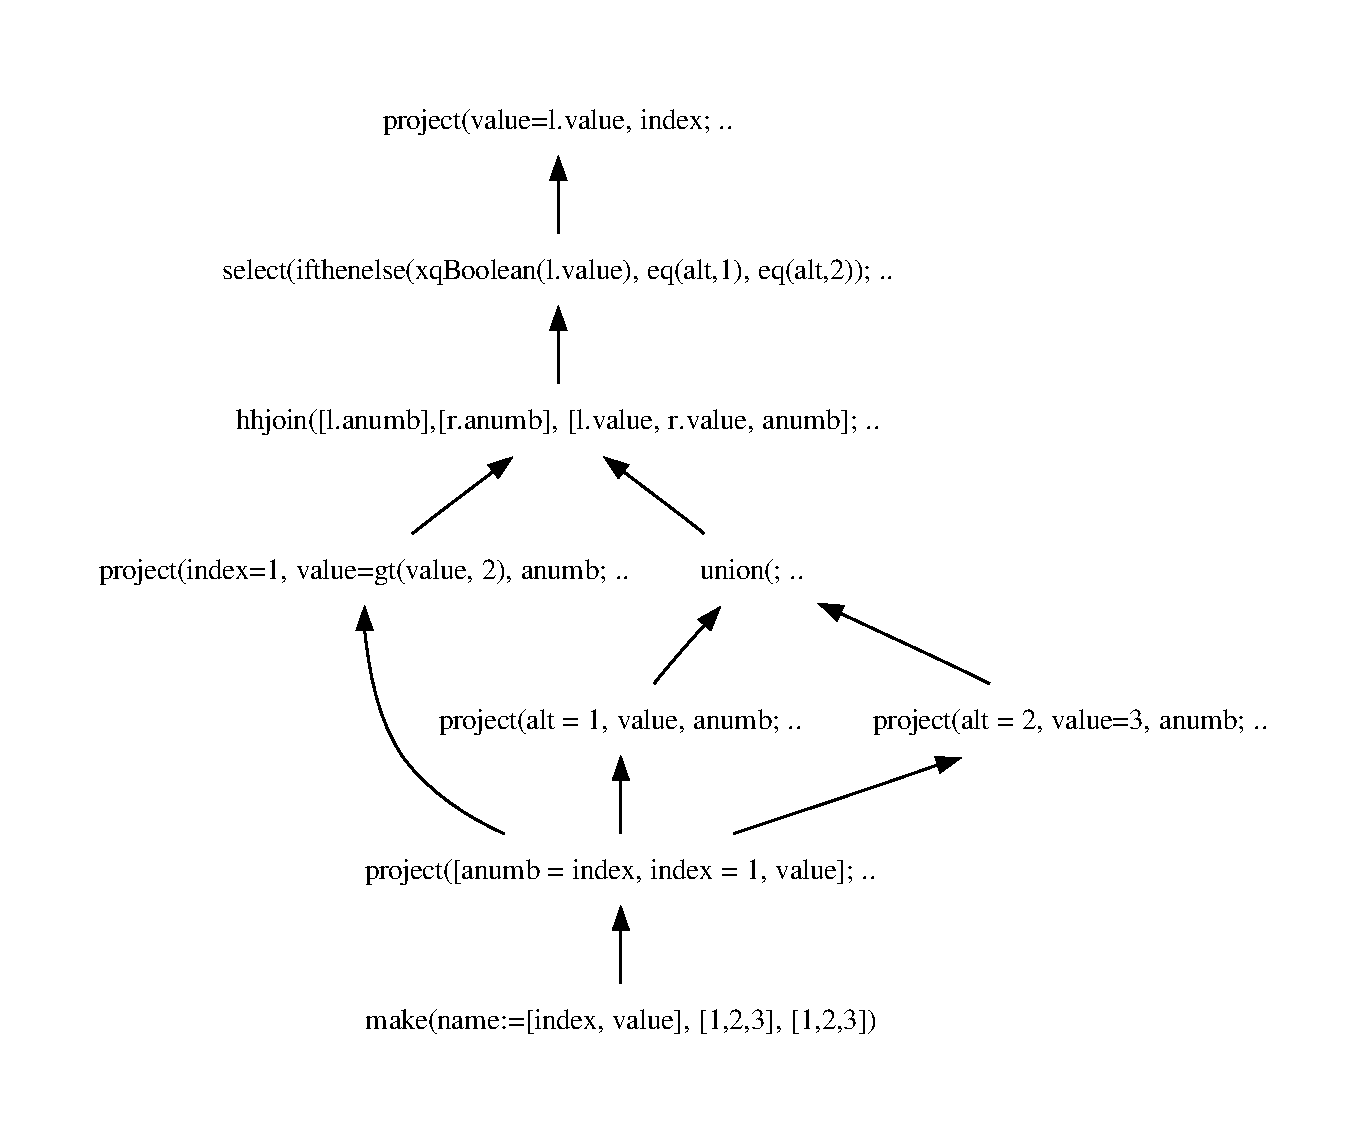
\includegraphics[width=1.0\textwidth]{img/graphs/ifthenelse_dag}
  \caption{DAG representation of operator tree in figure
  \ref{fig:results:query_ifthenelse_result}}
  \label{fig:results:query_ifthenelse_result_dag}
\end{center}
\end{figure}

\newpage

\section{Algebra Generated By Implementation}
\label{sect:result:implementation_algebra}
In this section, a collection of trivial queries are translated to relational
algebra using the implemented proof of concept described in chapter
\ref{chapter:implementation}. Naturally, this implementation also uses the
``Tainting Dependencies'' method, however the results from these translations
can also be used in a comparison with loop lifting.

\subsection{Trivial FLWOR}
\label{sect:results:algebra:generated:trivial_flwor}
\subsubsection{Query premise}
\begin{figure}[!htp]
\begin{center}
\begin{Verbatim}
for $a in (1,2,3) return $a
\end{Verbatim}
  \caption{Trivial FLWOR query premise}
  \label{fig:results:query_trivial_flwor}
\end{center}
\end{figure}

\subsubsection{Result}
\begin{figure}[!htp]
\begin{center}
  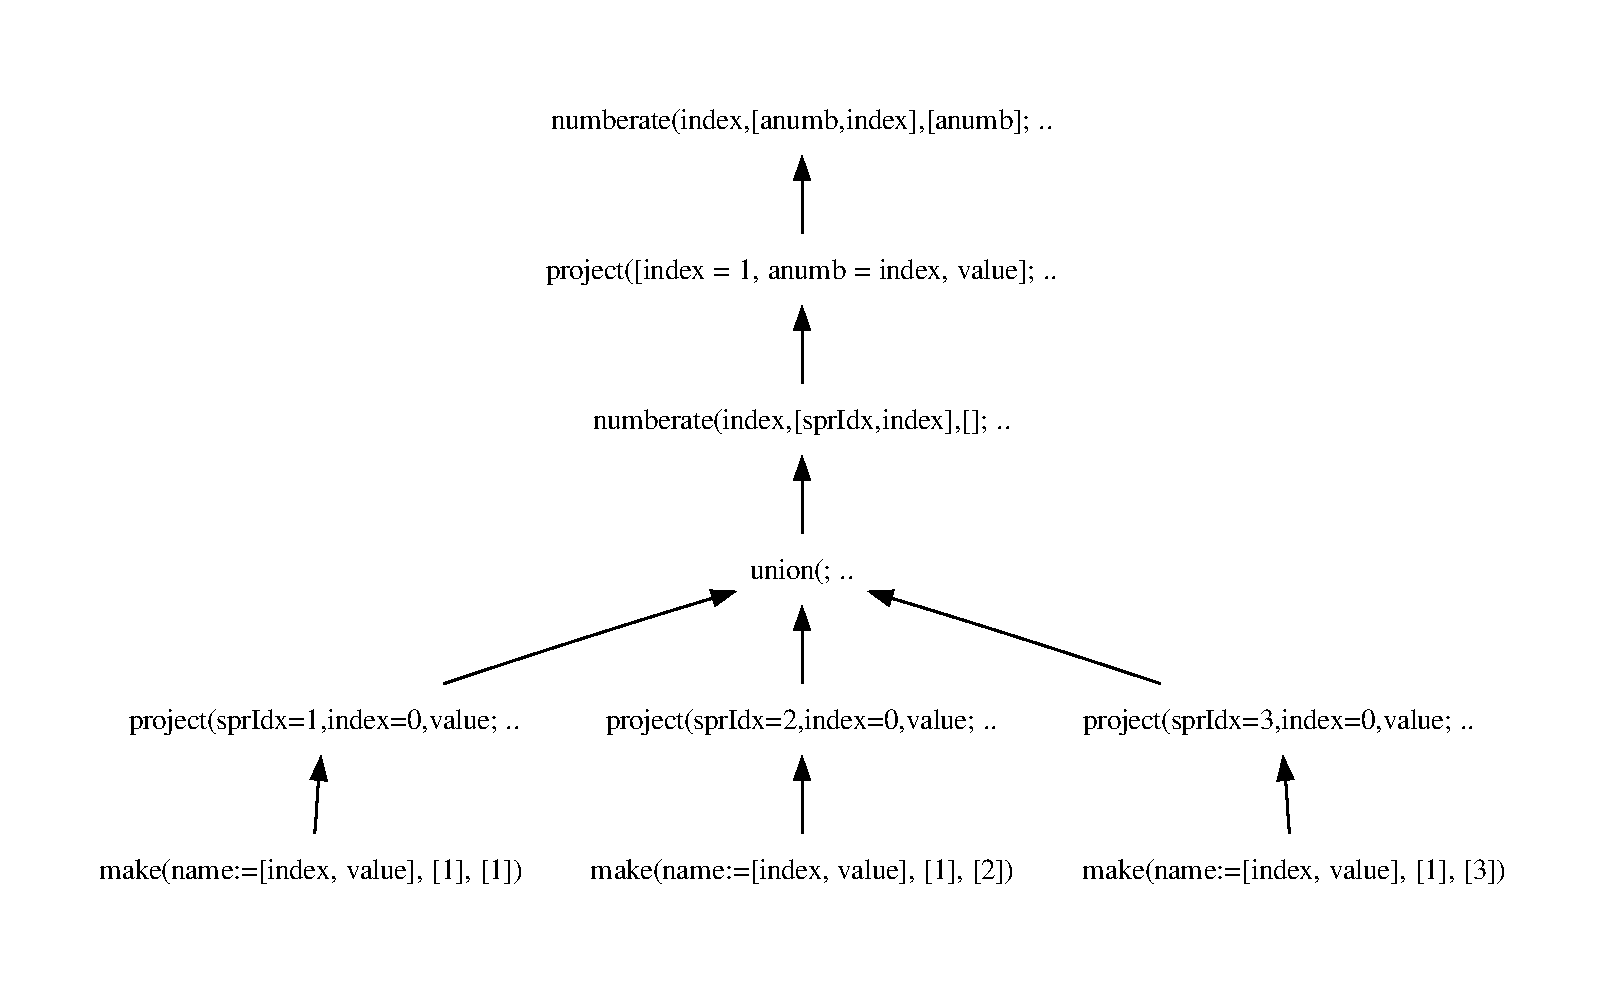
\includegraphics[width=1.0\textwidth]{img/graphs/td_impl_flwor_simple_xq_relalg} \caption{Complete translation of expression in figure
  \ref{fig:results:query_trivial_flwor}}
  \label{fig:results:query_trivial_flwor_result}
\end{center}
\end{figure}

\subsection{Complex FLWOR}
\label{sect:results:algebra:generated:complex_flwor}
\subsubsection{Query premise}
\begin{figure}[!htp]
\begin{center}
\begin{Verbatim}
for $a in (1,2) return (3, for $b in (4,5) return ($a, $b, 6))
\end{Verbatim}
  \caption{Complex FLWOR query premise}
  \label{fig:results:query_complex_flwor}
\end{center}
\end{figure}

\subsubsection{Result}
\begin{figure}[!htp]
\begin{center}
  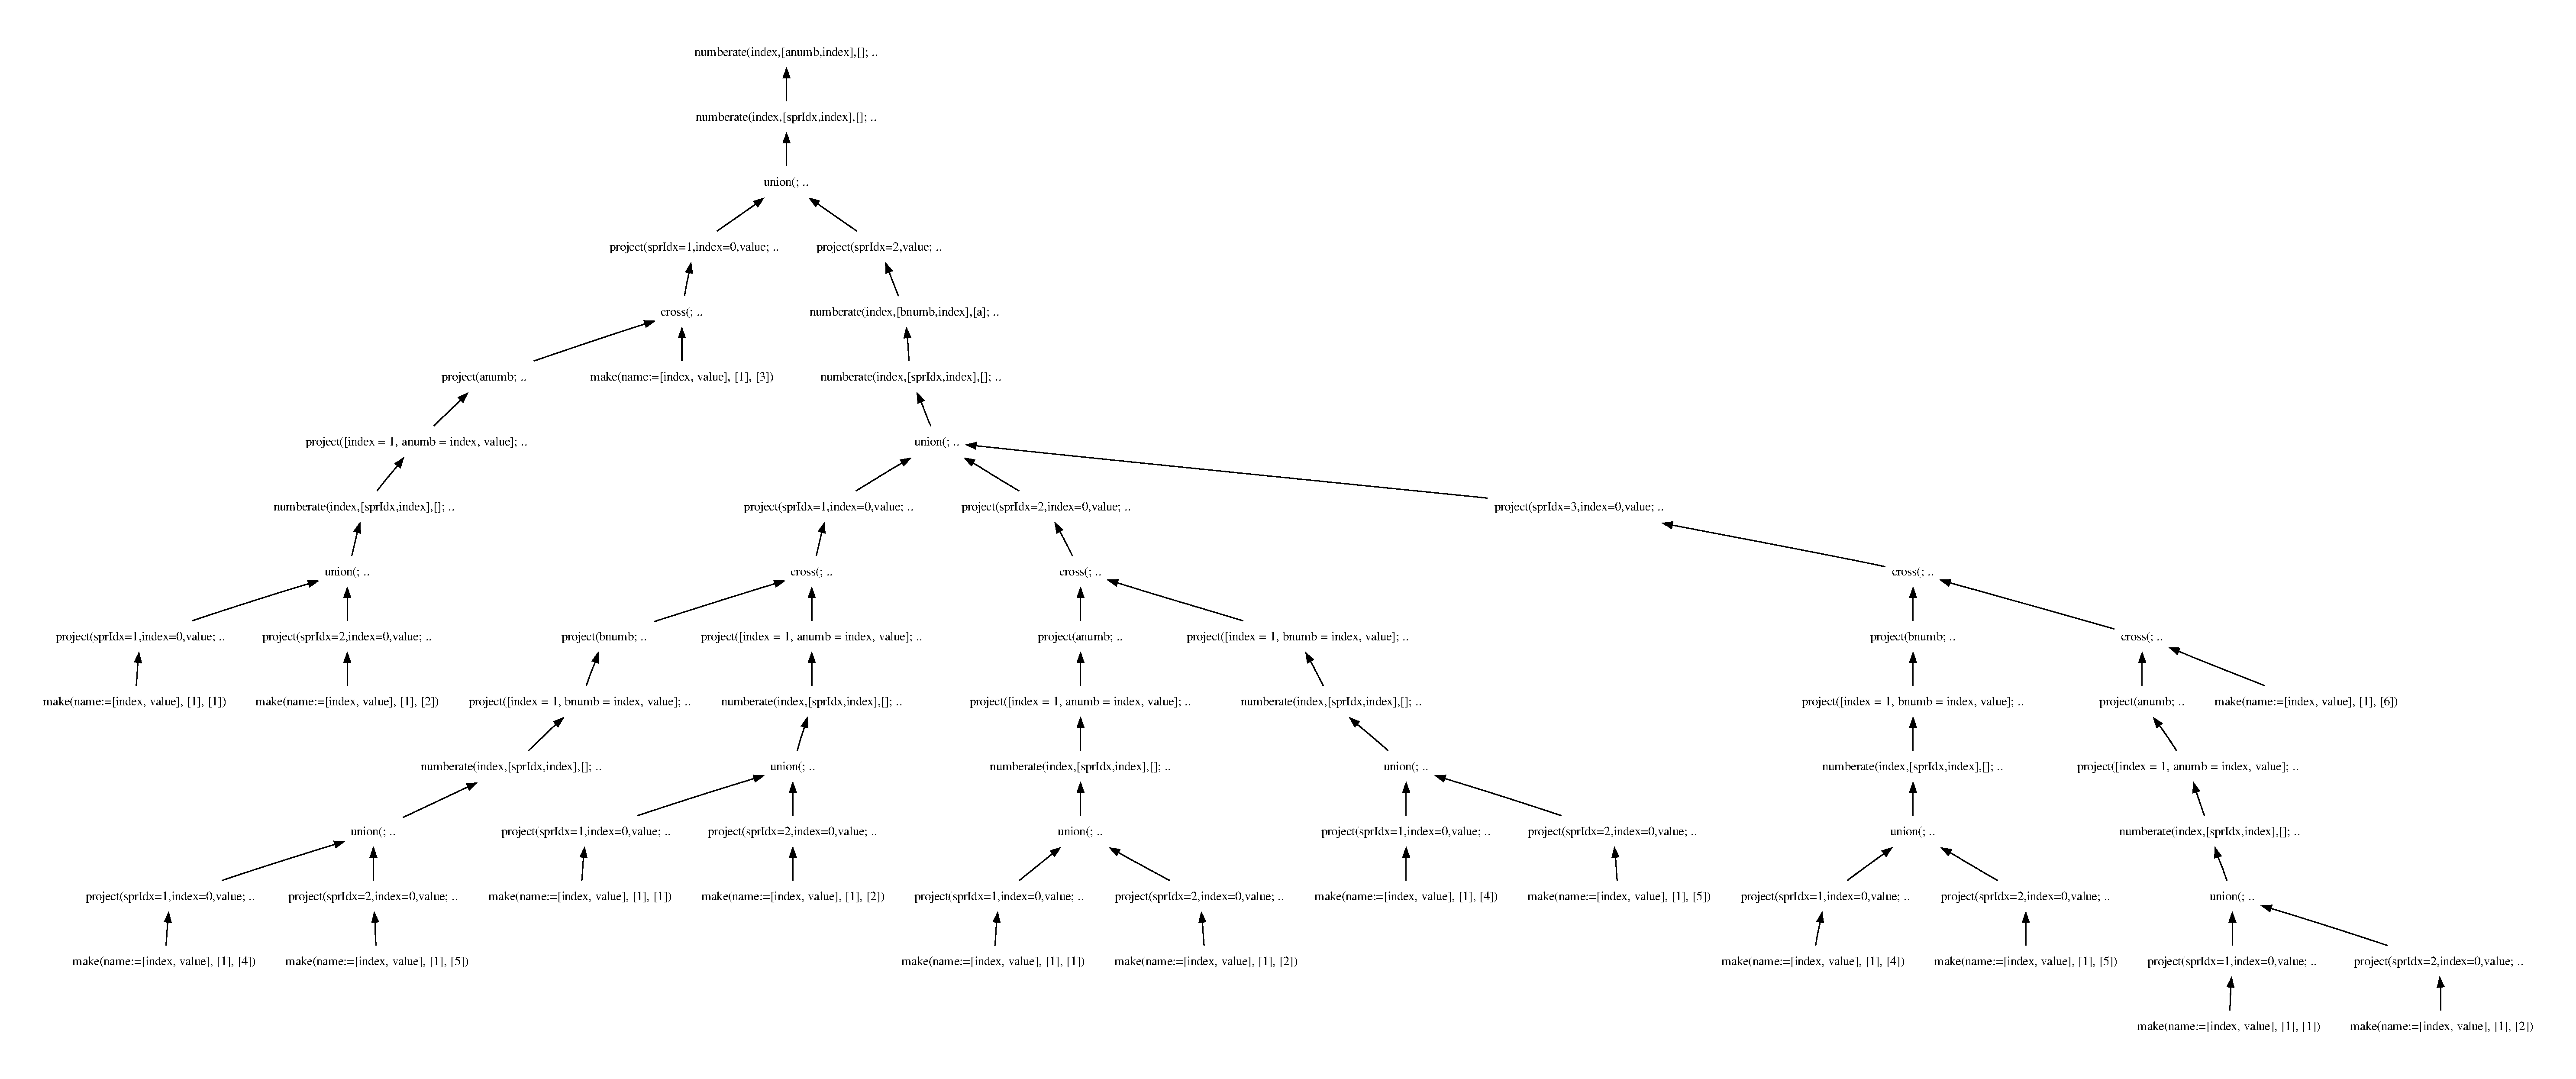
\includegraphics[angle=90,height=0.7\textheight]{img/graphs/td_impl_flwor_complex_xq_relalg} \caption{Complete
  translation of expression in figure
  \ref{fig:results:query_complex_flwor}}
  \label{fig:results:query_complex_flwor_result}
\end{center}
\end{figure}


The algebra tree in figure \ref{fig:results:query_complex_flwor_result} can
be converted to the DAG in figure
\ref{fig:results:query_complex_flwor_result_dag}

\begin{figure}[!htp]
\begin{center}
  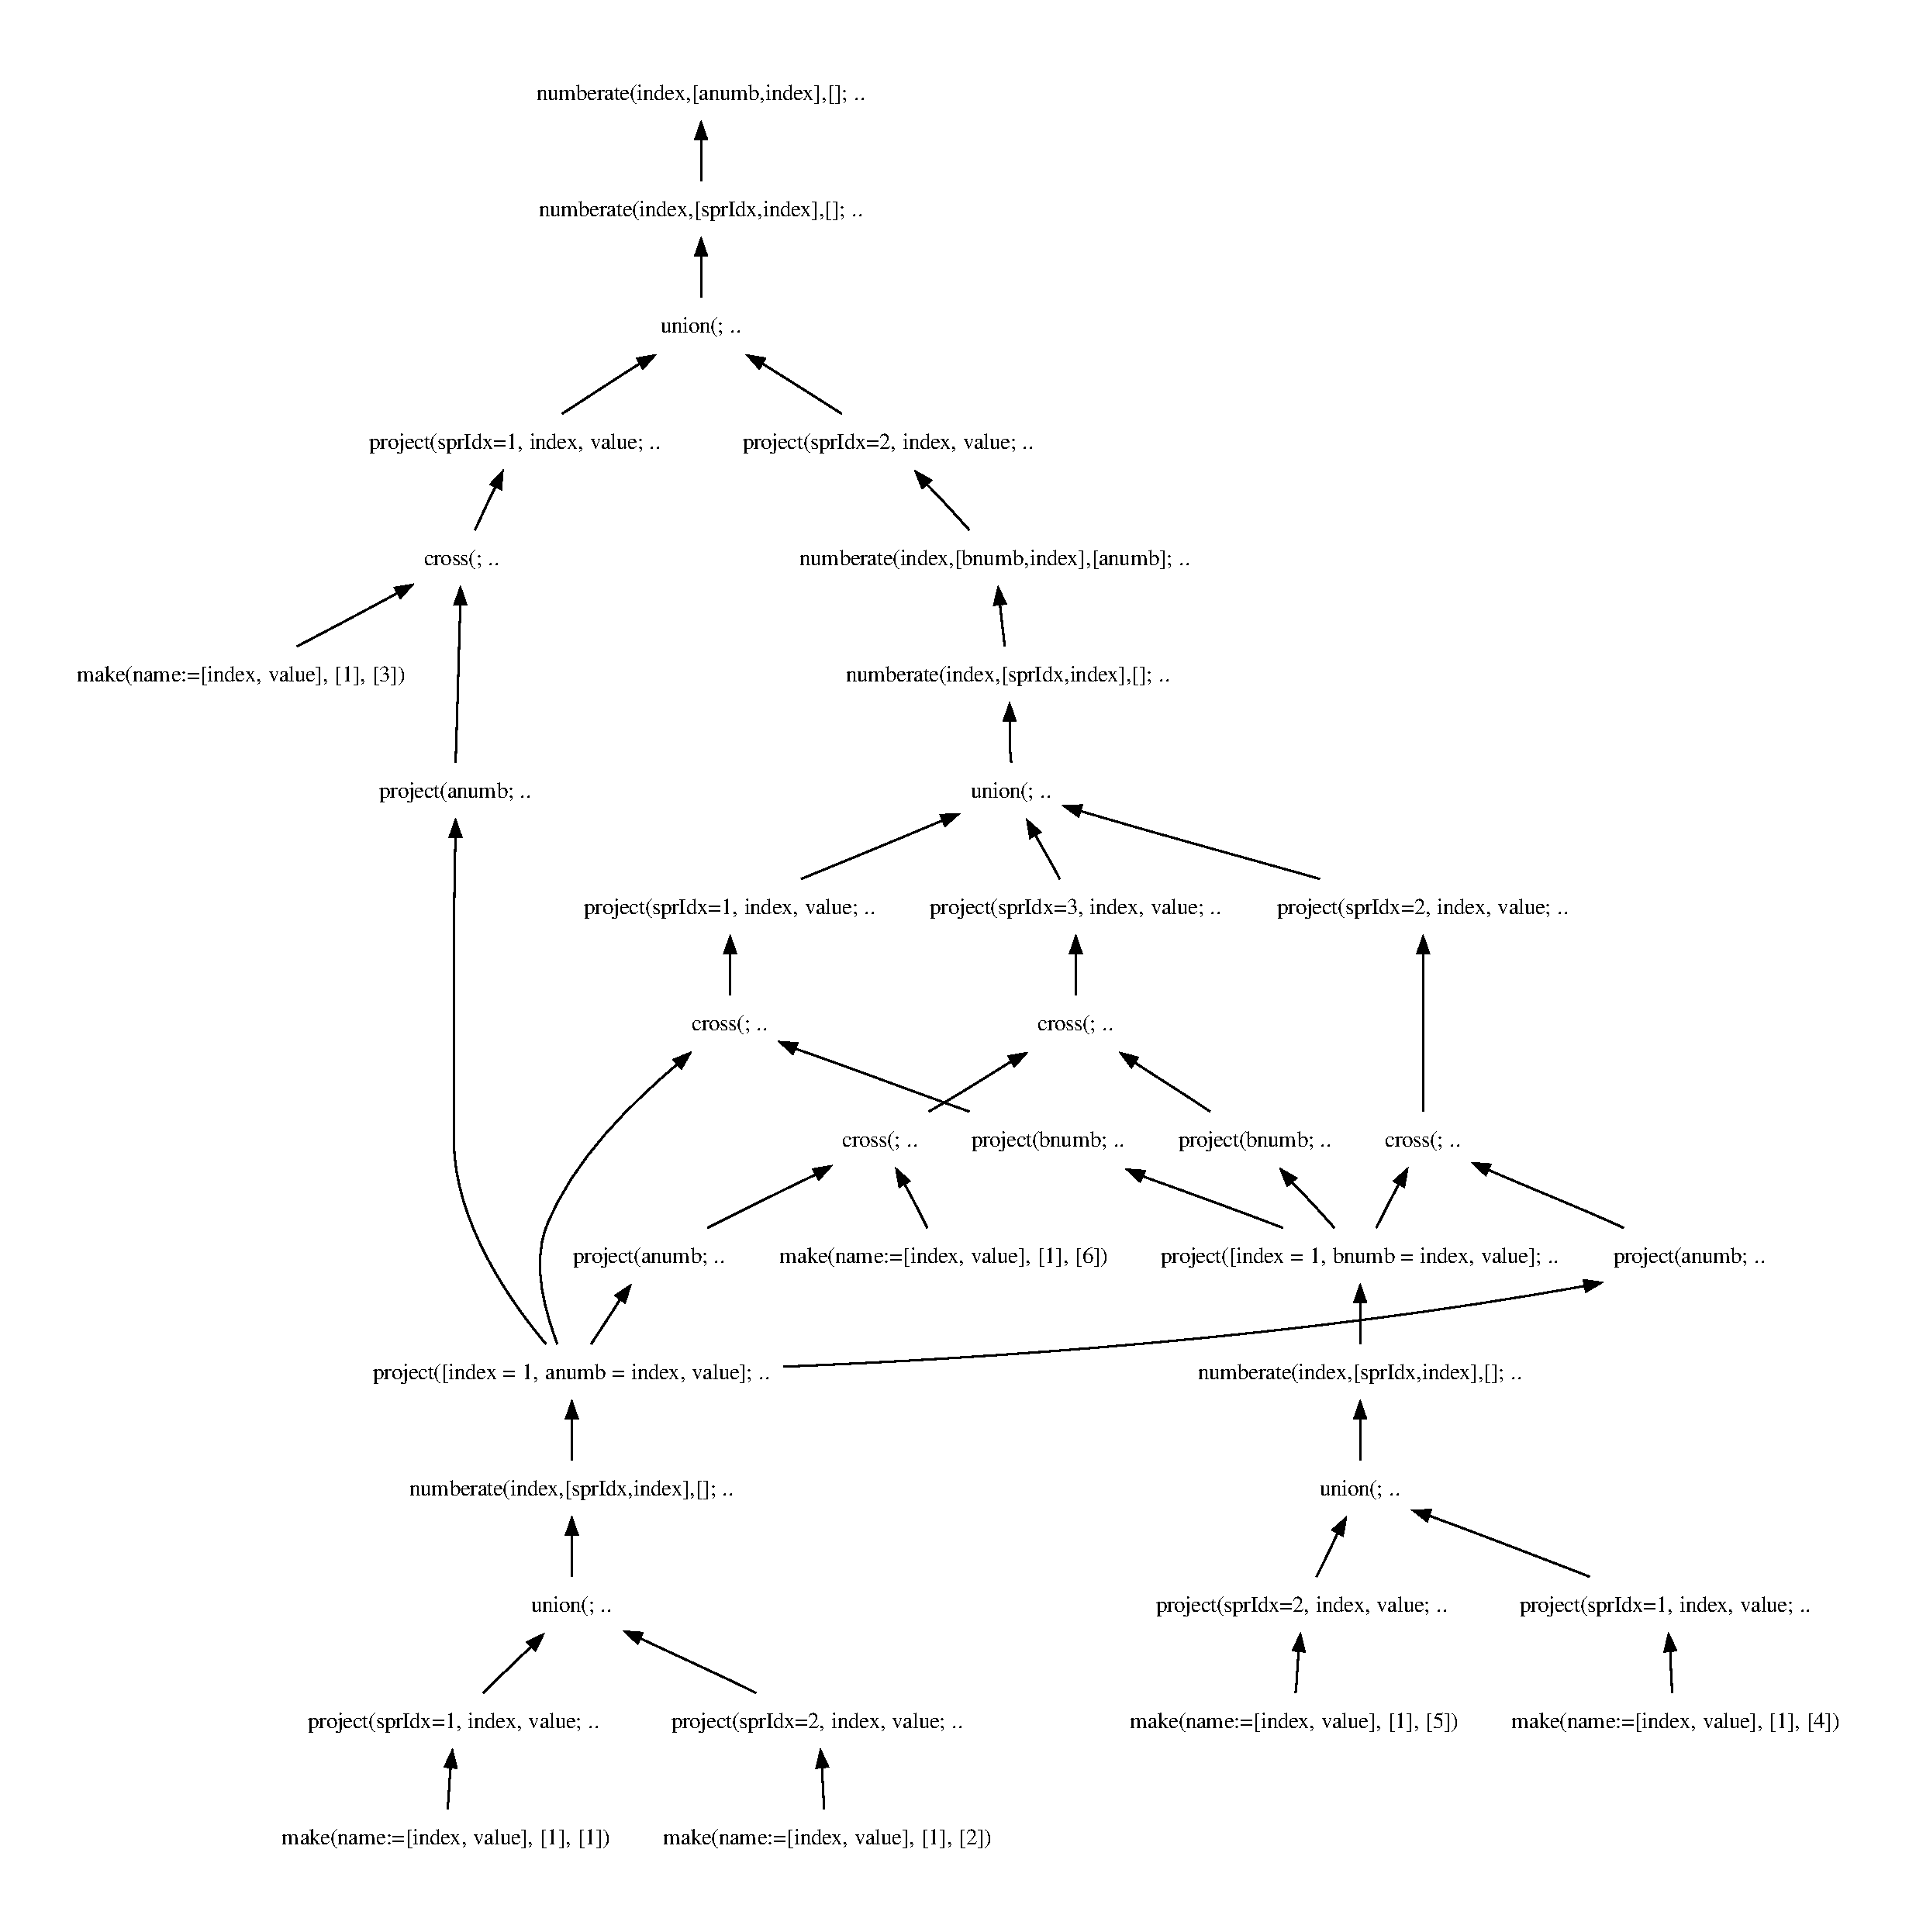
\includegraphics[width=1.0\textwidth]{img/graphs/td_impl_flwor_complex_xq_relalg_dag}
  \caption{Complete translation of expression in figure
  \ref{fig:results:query_complex_flwor} converted to a DAG}
  \label{fig:results:query_complex_flwor_result_dag}
\end{center}
\end{figure}
\newpage

\subsection{FLWOR with conditional}
\label{sect:results:algebra:generated:conditional_flwor}
\subsubsection{Query premise}
\begin{figure}[!htp]
\begin{center}
\begin{Verbatim}
for $a in (10,20) return if ($a > 15) then $a else 15
\end{Verbatim}
  \caption{Conditional FLWOR query premise}
  \label{fig:results:query_conditional_flwor}
\end{center}
\end{figure}

\subsubsection{Result}
\begin{figure}[!htp]
\begin{center}
  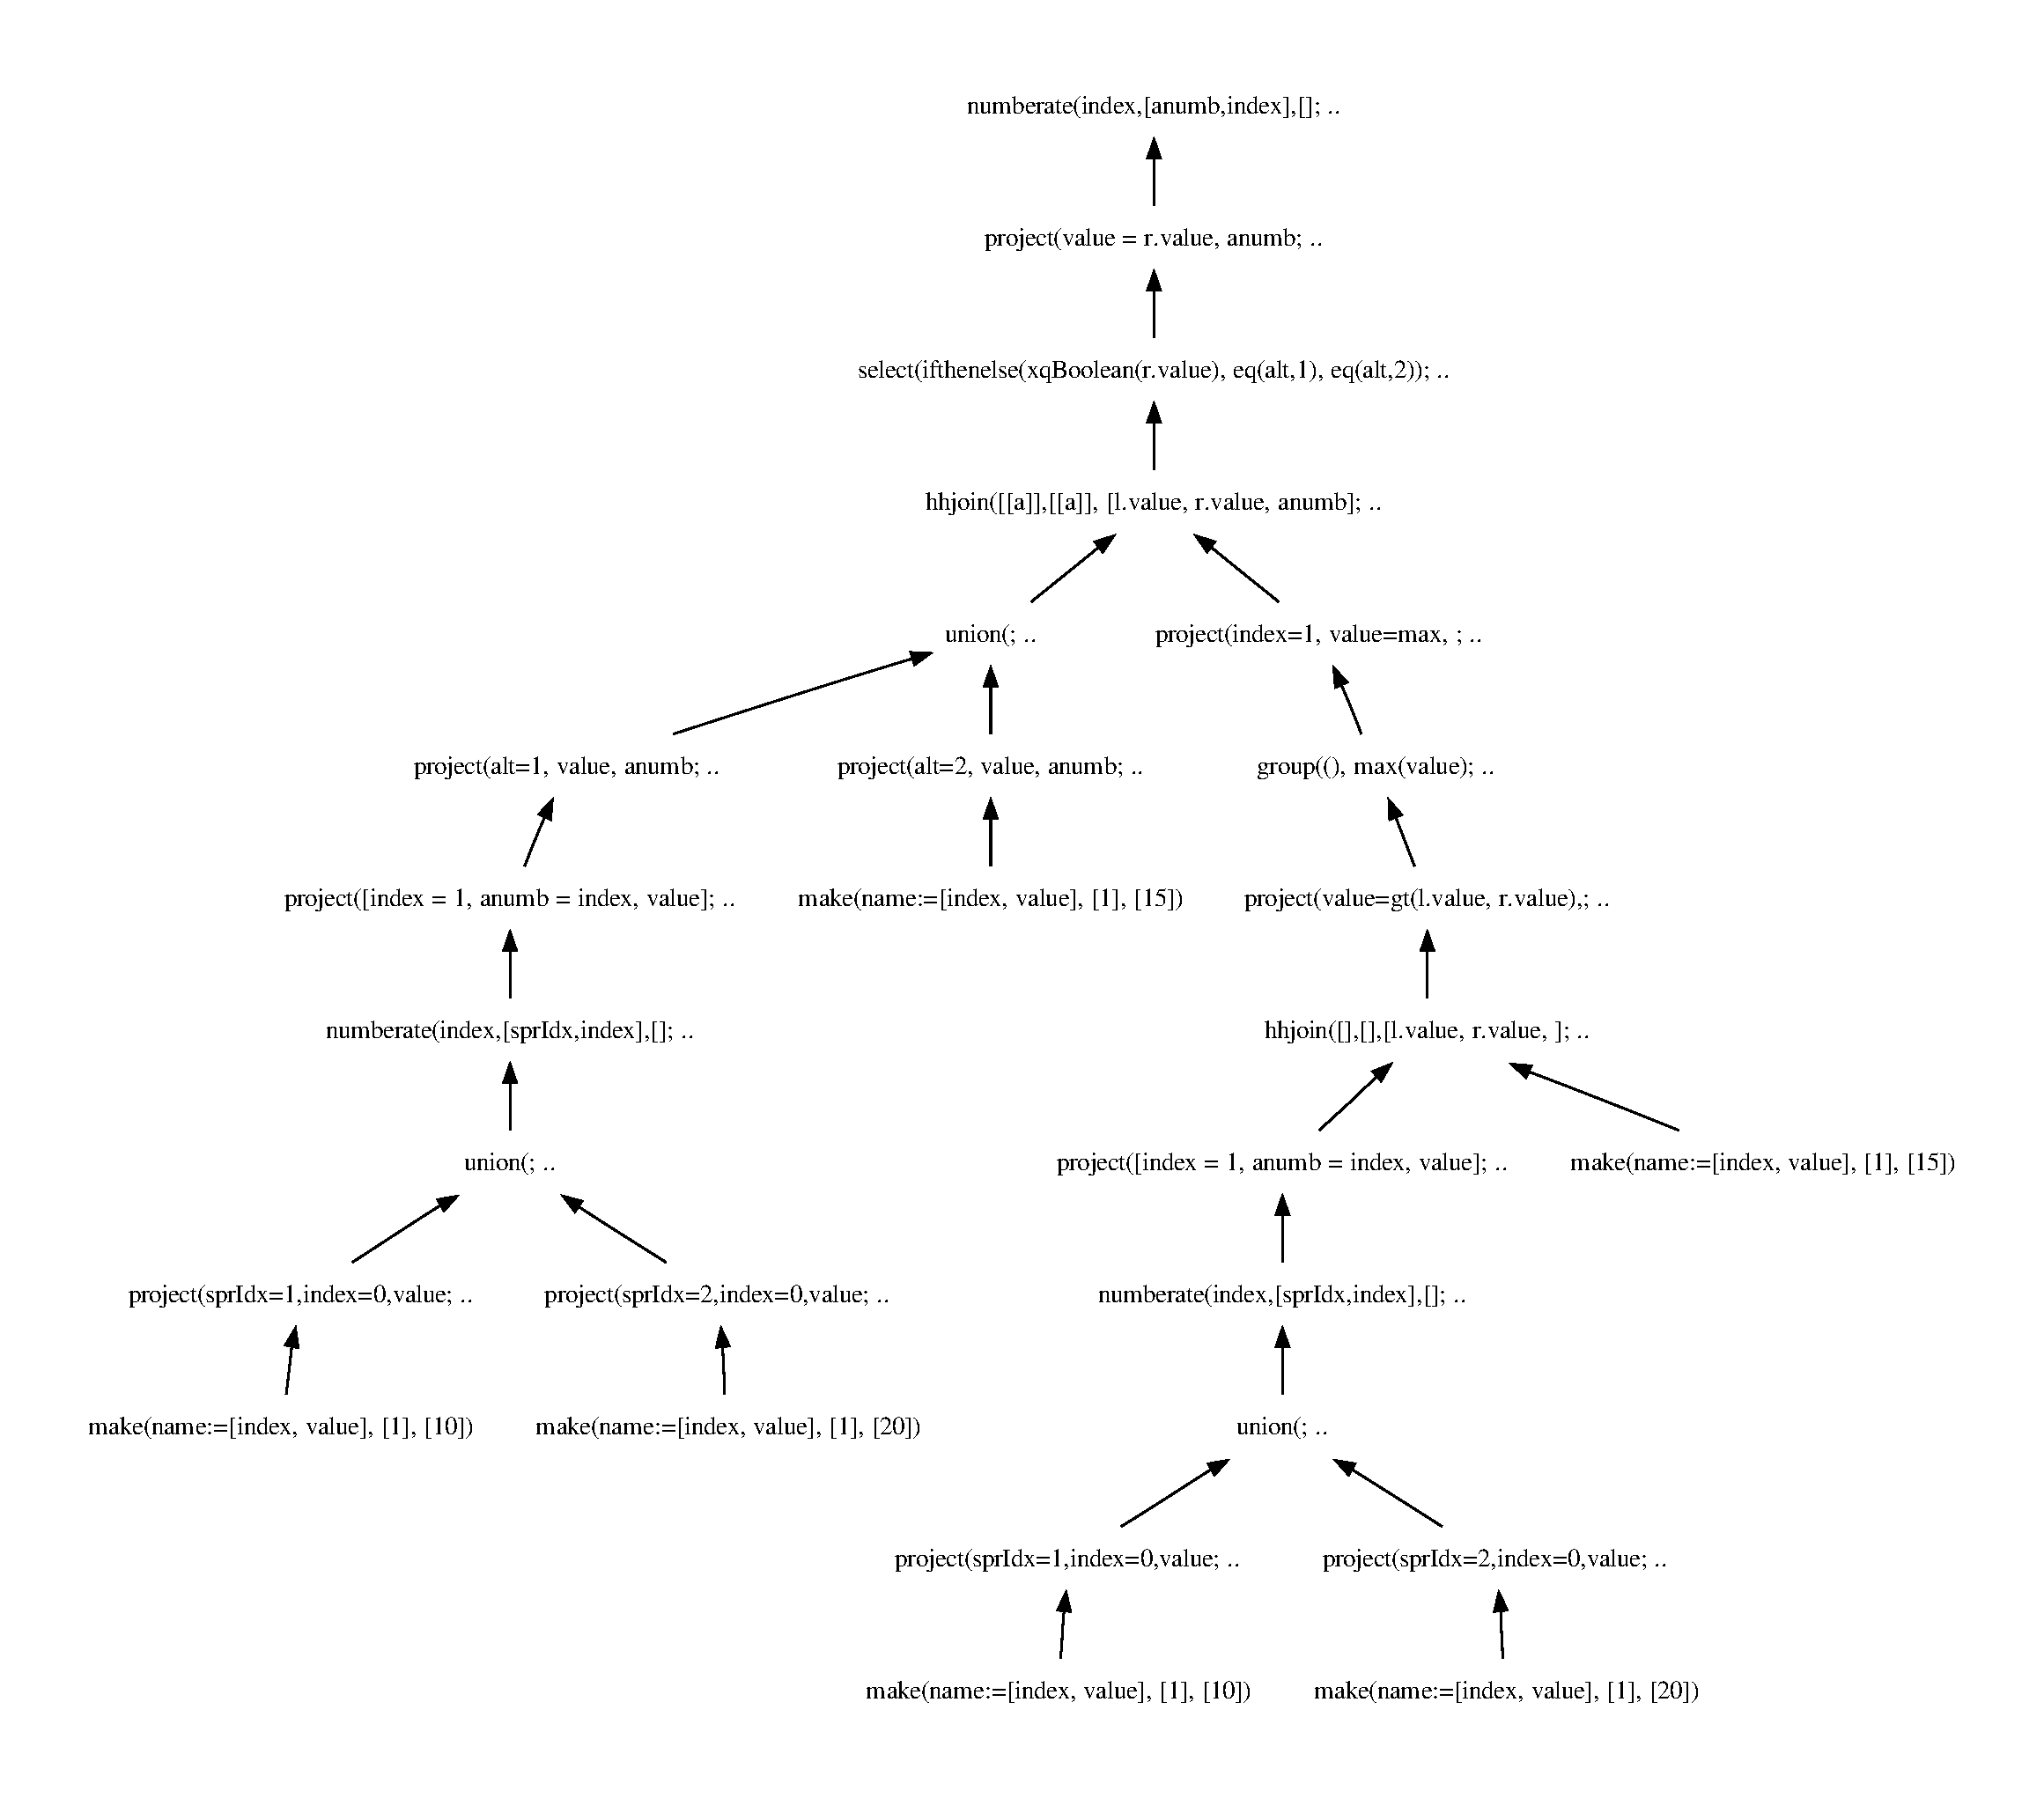
\includegraphics[width=1.0\textwidth]{img/graphs/td_impl_flwor_ifthenelse_xq_relalg}
  \caption{Complete translation of expression in figure
  \ref{fig:results:query_conditional_flwor}}
  \label{fig:results:query_conditional_flwor_result}
\end{center}
\end{figure}

The algebra tree in figure \ref{fig:results:query_conditional_flwor_result} can
be converted to the DAG in figure
\ref{fig:results:query_conditional_flwor_result_dag}

\newpage
\begin{figure}[!htp]
\begin{center} 
  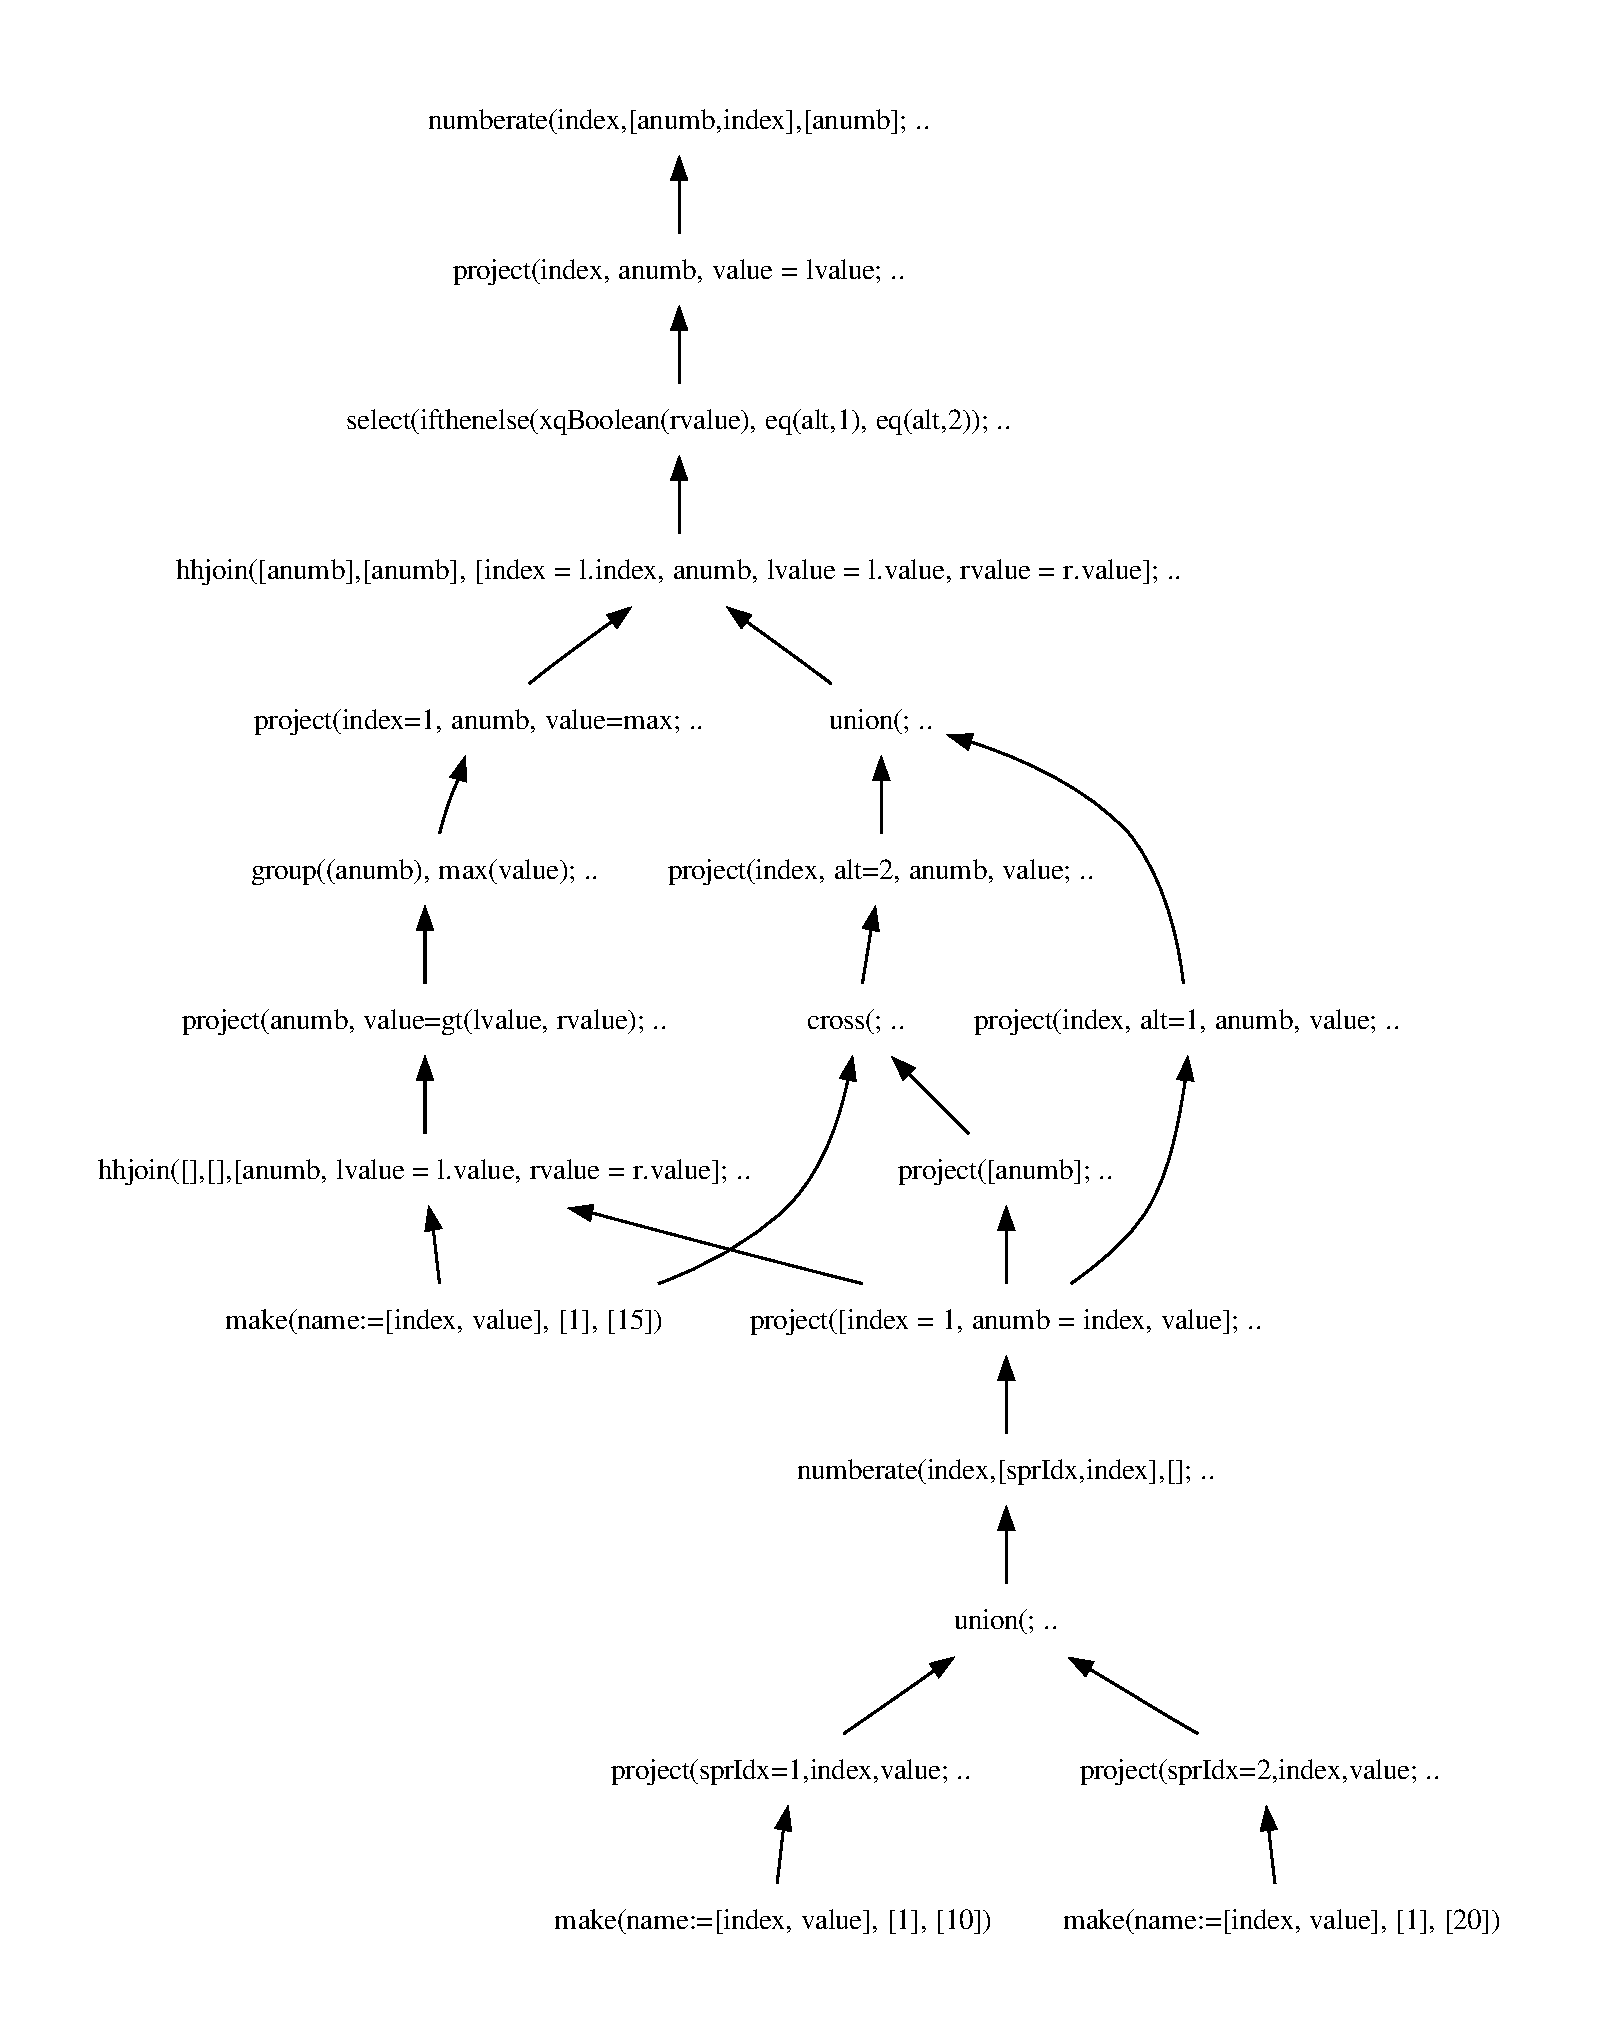
\includegraphics[width=1.0\textwidth]{img/graphs/td_impl_flwor_ifthenelse_xq_relalg_dag}
  \caption{Complete translation of expression in figure
  \ref{fig:results:query_conditional_flwor} converted to a DAG}
  \label{fig:results:query_conditional_flwor_result_dag}
\end{center}
\end{figure}
\section{Comparison}
\label{sect:results:comparison}
\subsection{Assumptions}
This comparison must be seen in the context of a number of assumptions
about the systems being compared. With regards to fairness, it is important to
note that the algebra trees generated by Pathfinder may have been
optimised (to which the exact extent is not known), while the algebra trees
generated by the prototype developed throughout this project \emph{does not apply any optimalisations} at all. The
optimalisations applied by Pathfinder are noted
in \cite{pathfinder_purelyRelational}.

Some important effects on the Pathfinder algebra tree from these
optimalisations are:
\begin{itemize}
  \item The cartesian products between a loop relation and a constant
  subexpression are transformed into projections
  \item The custom operator \textsf{attach} is roughly a simpler equivalent to
  the \textsf{make()} operator in MQL (see section \ref{sect:method:mql}, page
  \pageref{sect:method:mql})
\end{itemize}
TODO: noe mer her?

\newpage
\subsection{DAG comparison}
Note that the readability for these DAG comparisons are not essential --
however, links to large-scale versions of these diagrams are noted in appendix
\ref{appendix:links_and_resources}.

\begin{figure}[!h]
	\centering
	\mbox{
		\subfigure[Pathfinder/MonetDB]{		
			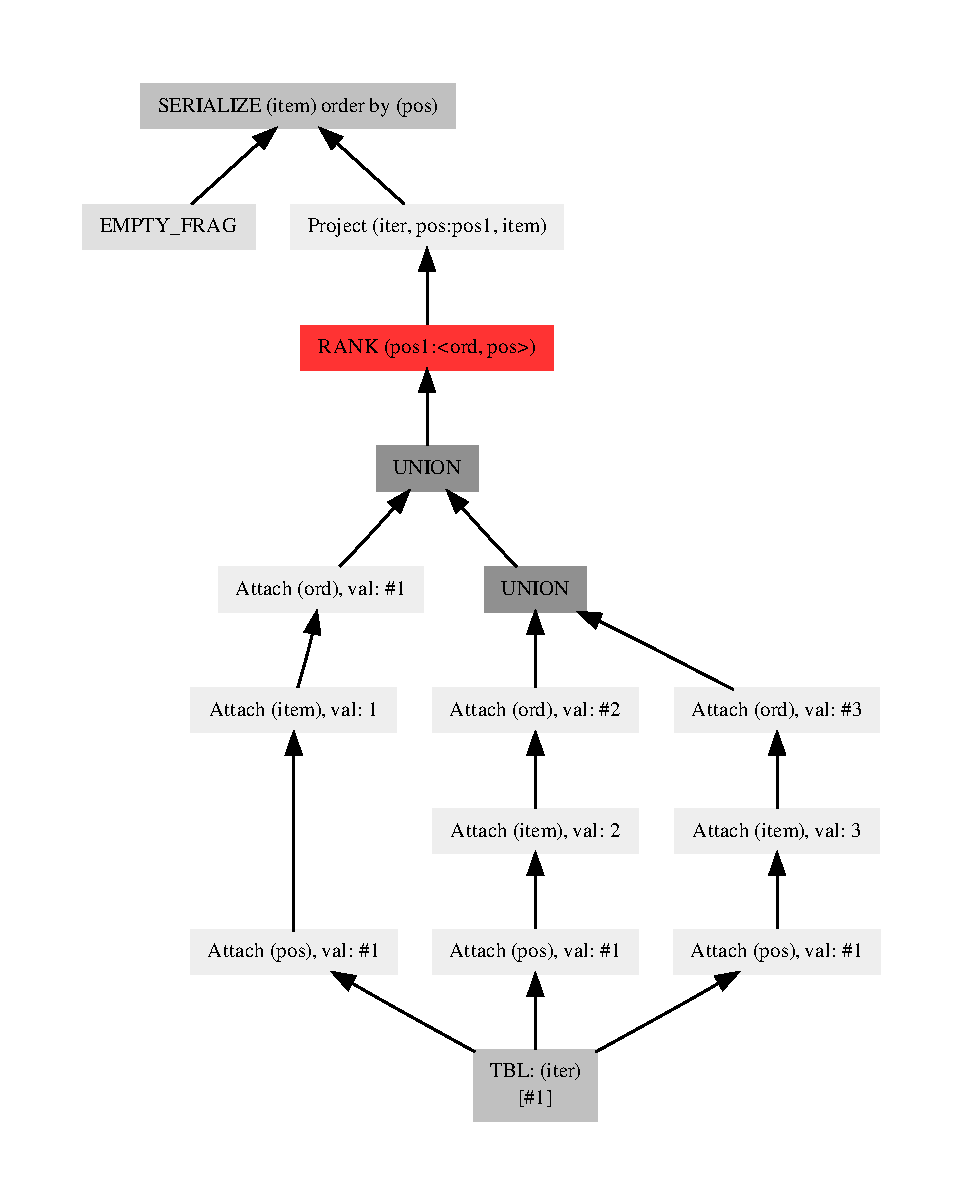
\includegraphics[width=0.4\textwidth]{img/graphs/td_impl_flwor_simple_pathfinder}
			\label{fig:result:comparison:simple_dag}
		}
		\quad
		\subfigure[Prototype implementation]{
		
			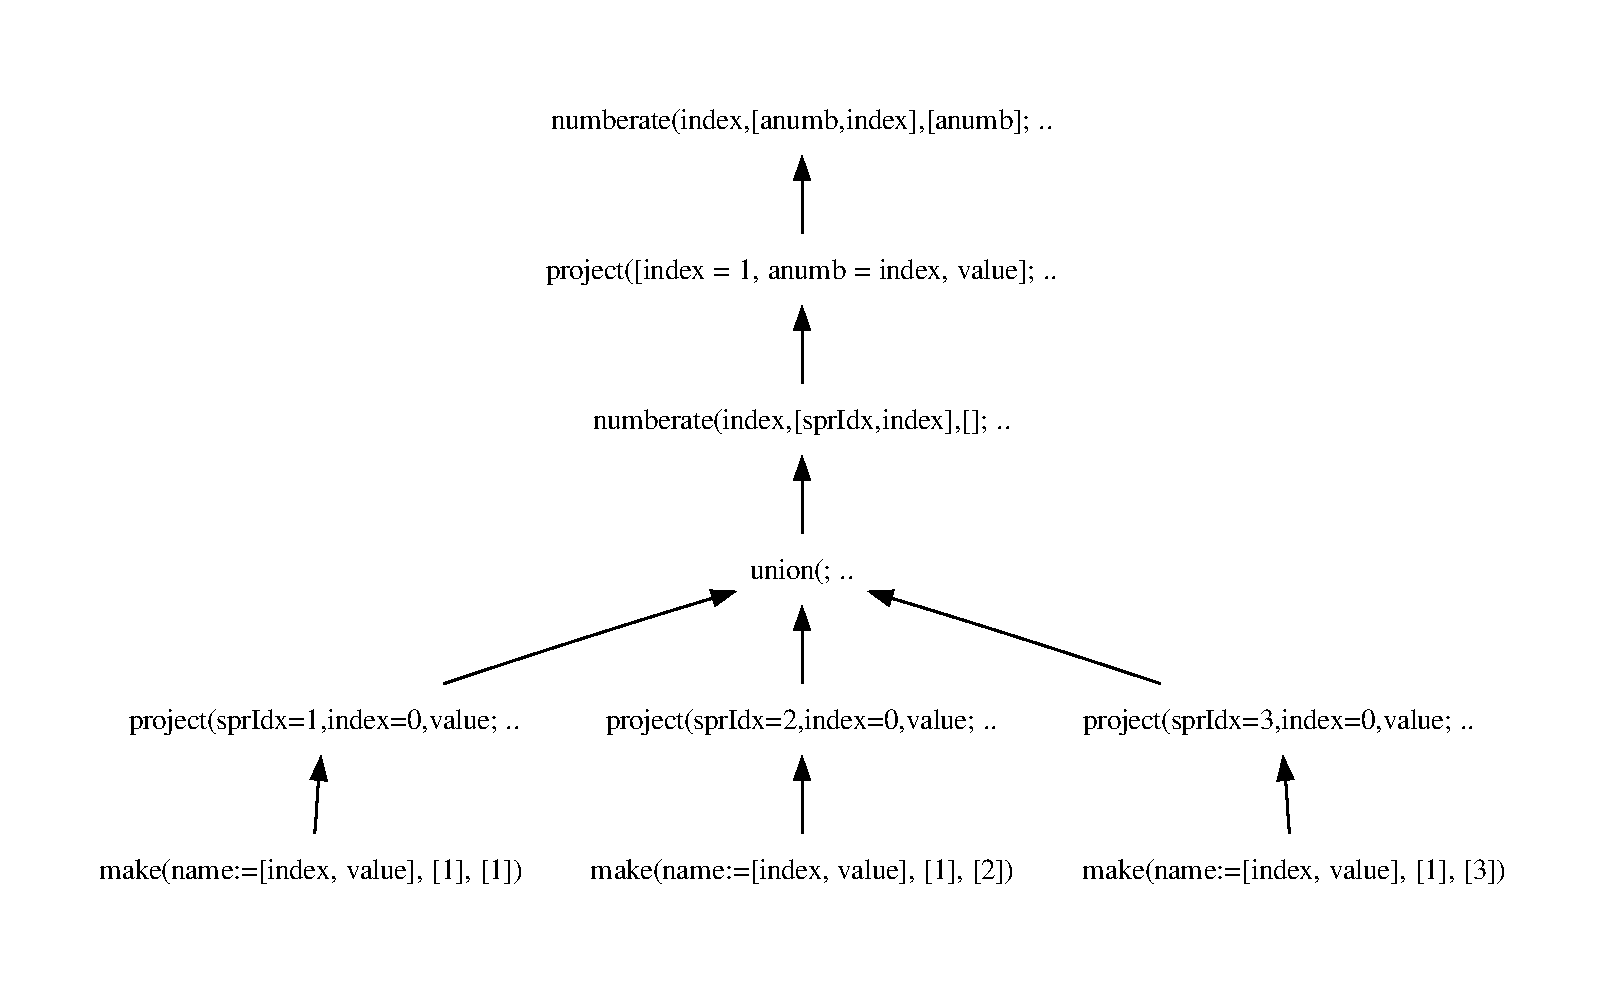
\includegraphics[width=0.6\textwidth]{img/graphs/td_impl_flwor_simple_xq_relalg}
			\label{fig:result:comparison:simple_pathfinder_dag}
		}
	}
	\caption{Comparison of DAGs for the trivial expression in section
	\ref{sect:results:algebra:generated:trivial_flwor}}
\end{figure}

\newpage
\begin{figure}[!h]
	\centering
	\mbox{
		\subfigure[Pathfinder/MonetDB]{		
			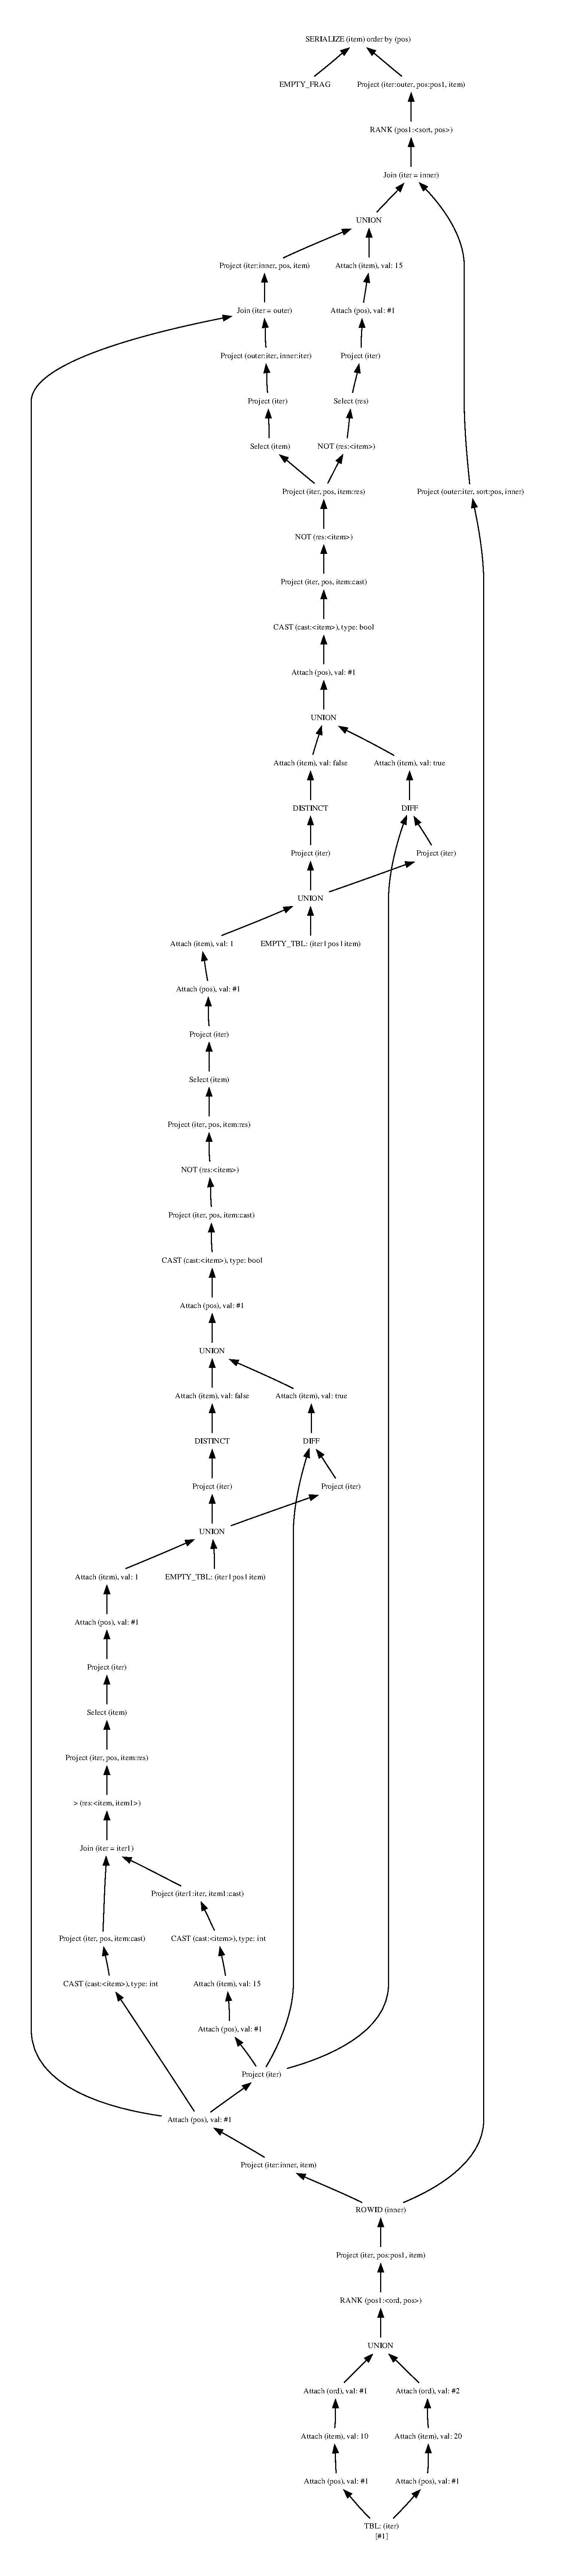
\includegraphics[width=0.3\textwidth]{img/graphs/td_impl_flwor_ifthenelse_pathfinder}
			\label{fig:result:comparison:conditional_dag}
		}
		\quad
		\subfigure[Prototype implementation]{
		
			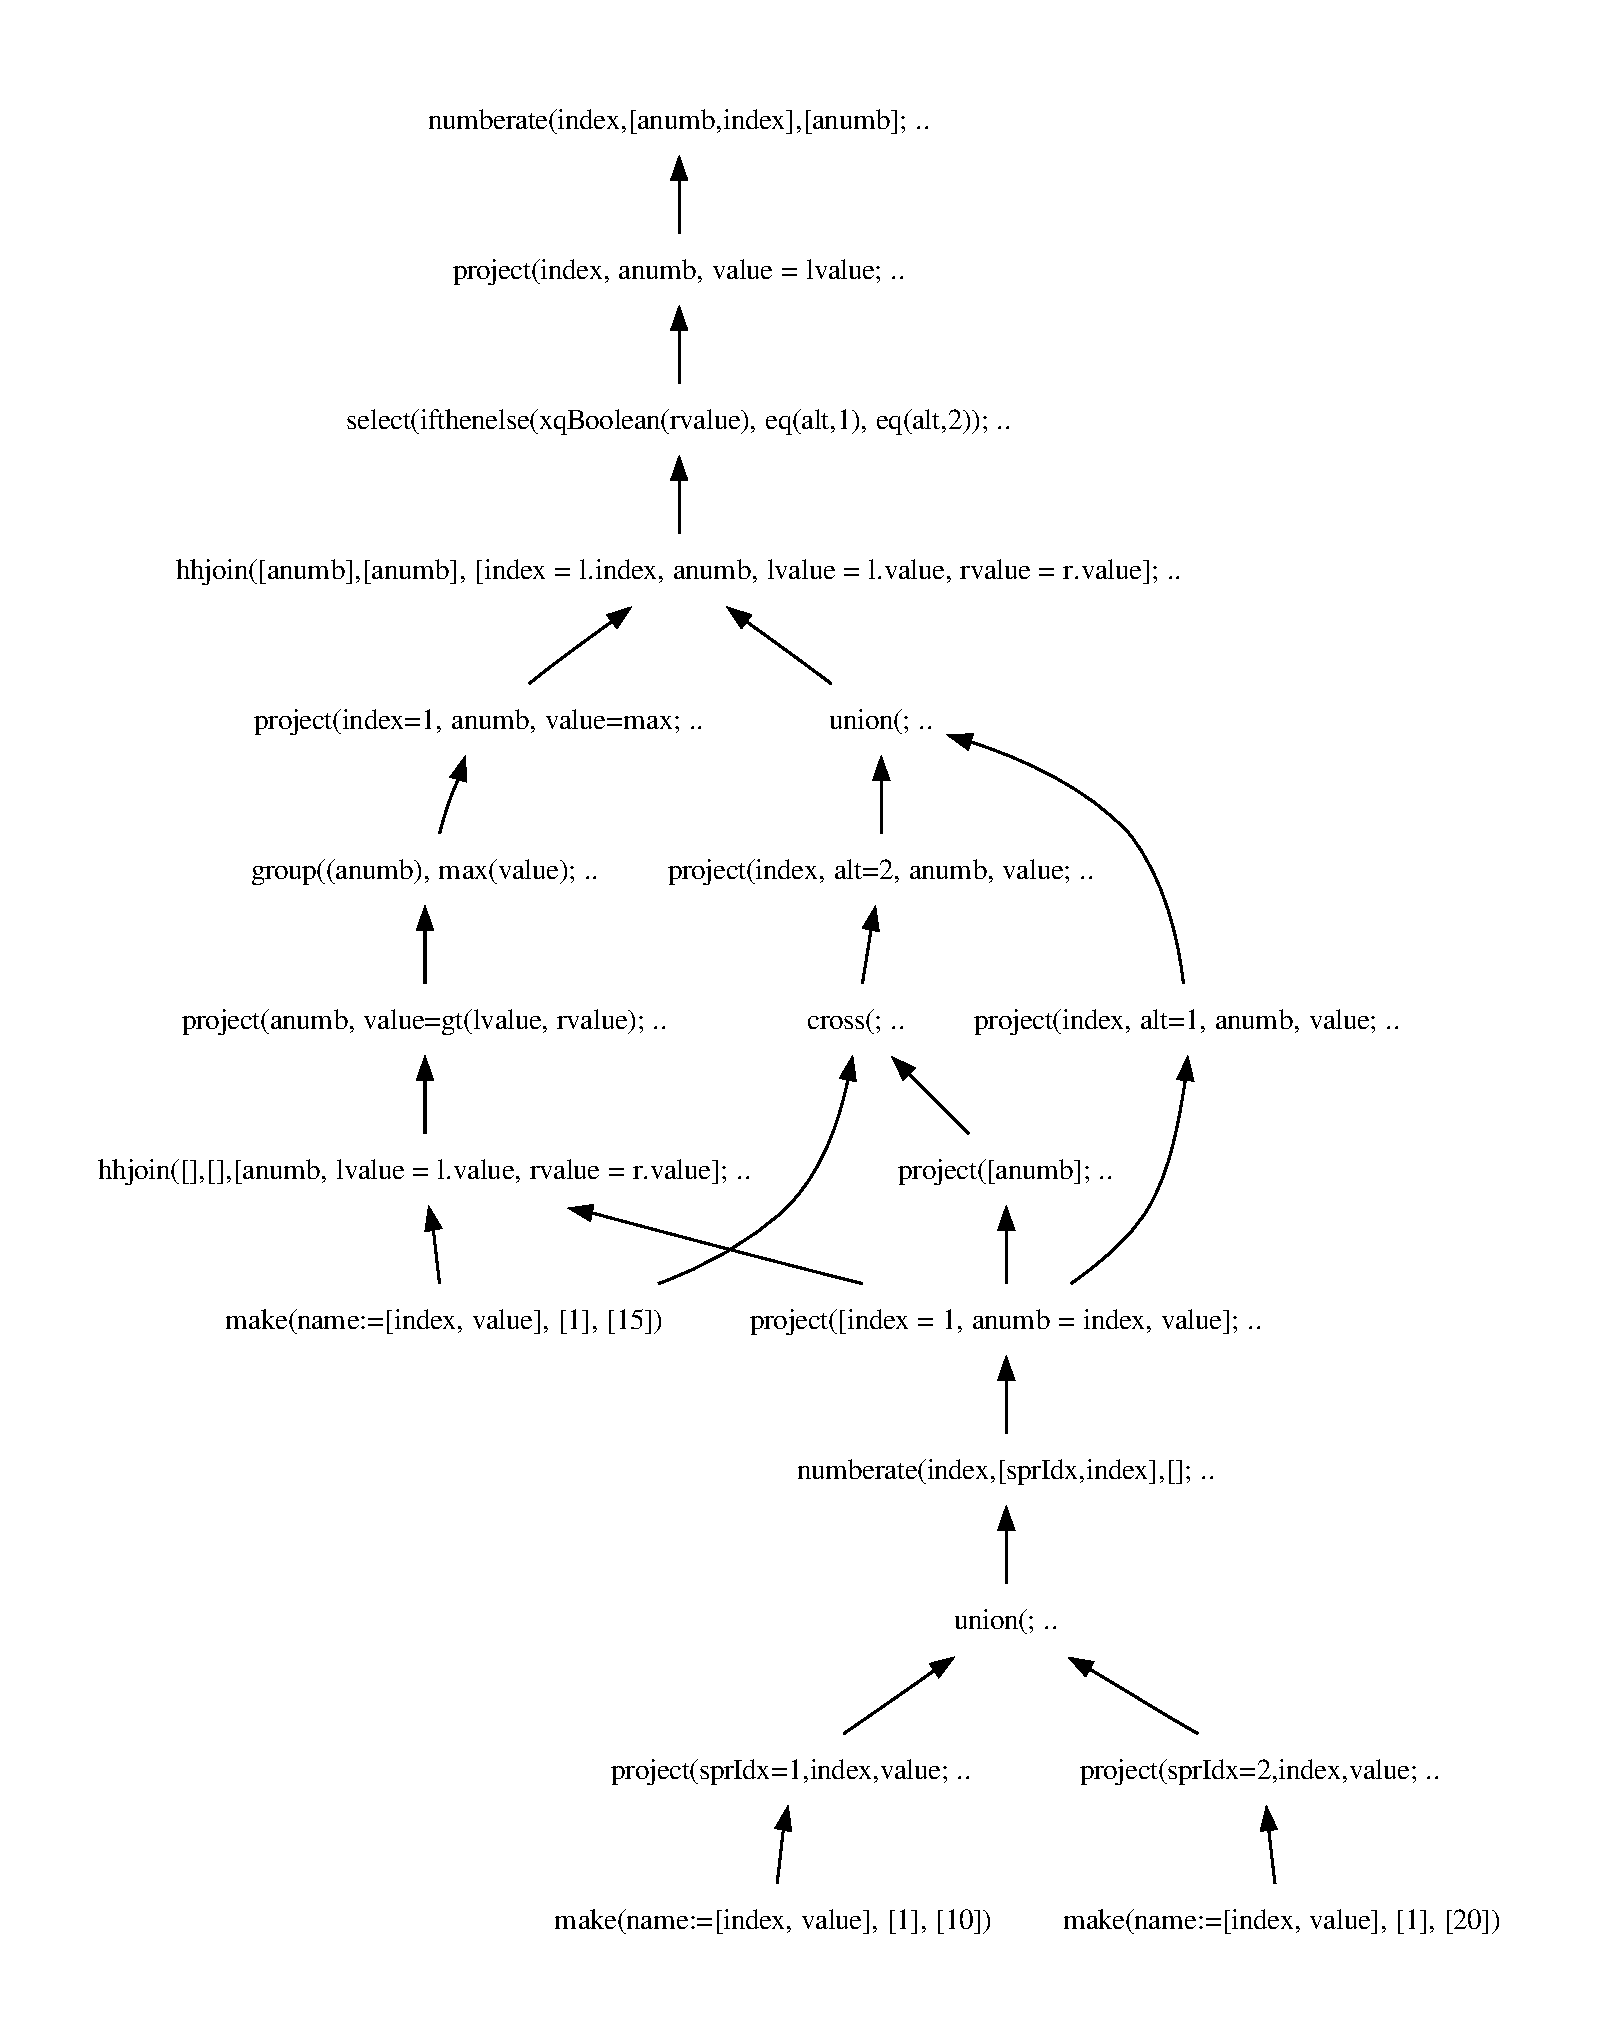
\includegraphics[width=0.7\textwidth]{img/graphs/td_impl_flwor_ifthenelse_xq_relalg_dag}
			\label{fig:result:comparison:conditional_pathfinder_dag}
		}
	}
	\caption{Comparison of DAGs for the conditional expression in section
	\ref{sect:results:algebra:generated:conditional_flwor}}
\end{figure}

\newpage
\begin{figure}[!h]
	\centering
	\mbox{
		\subfigure[Pathfinder/MonetDB]{		
			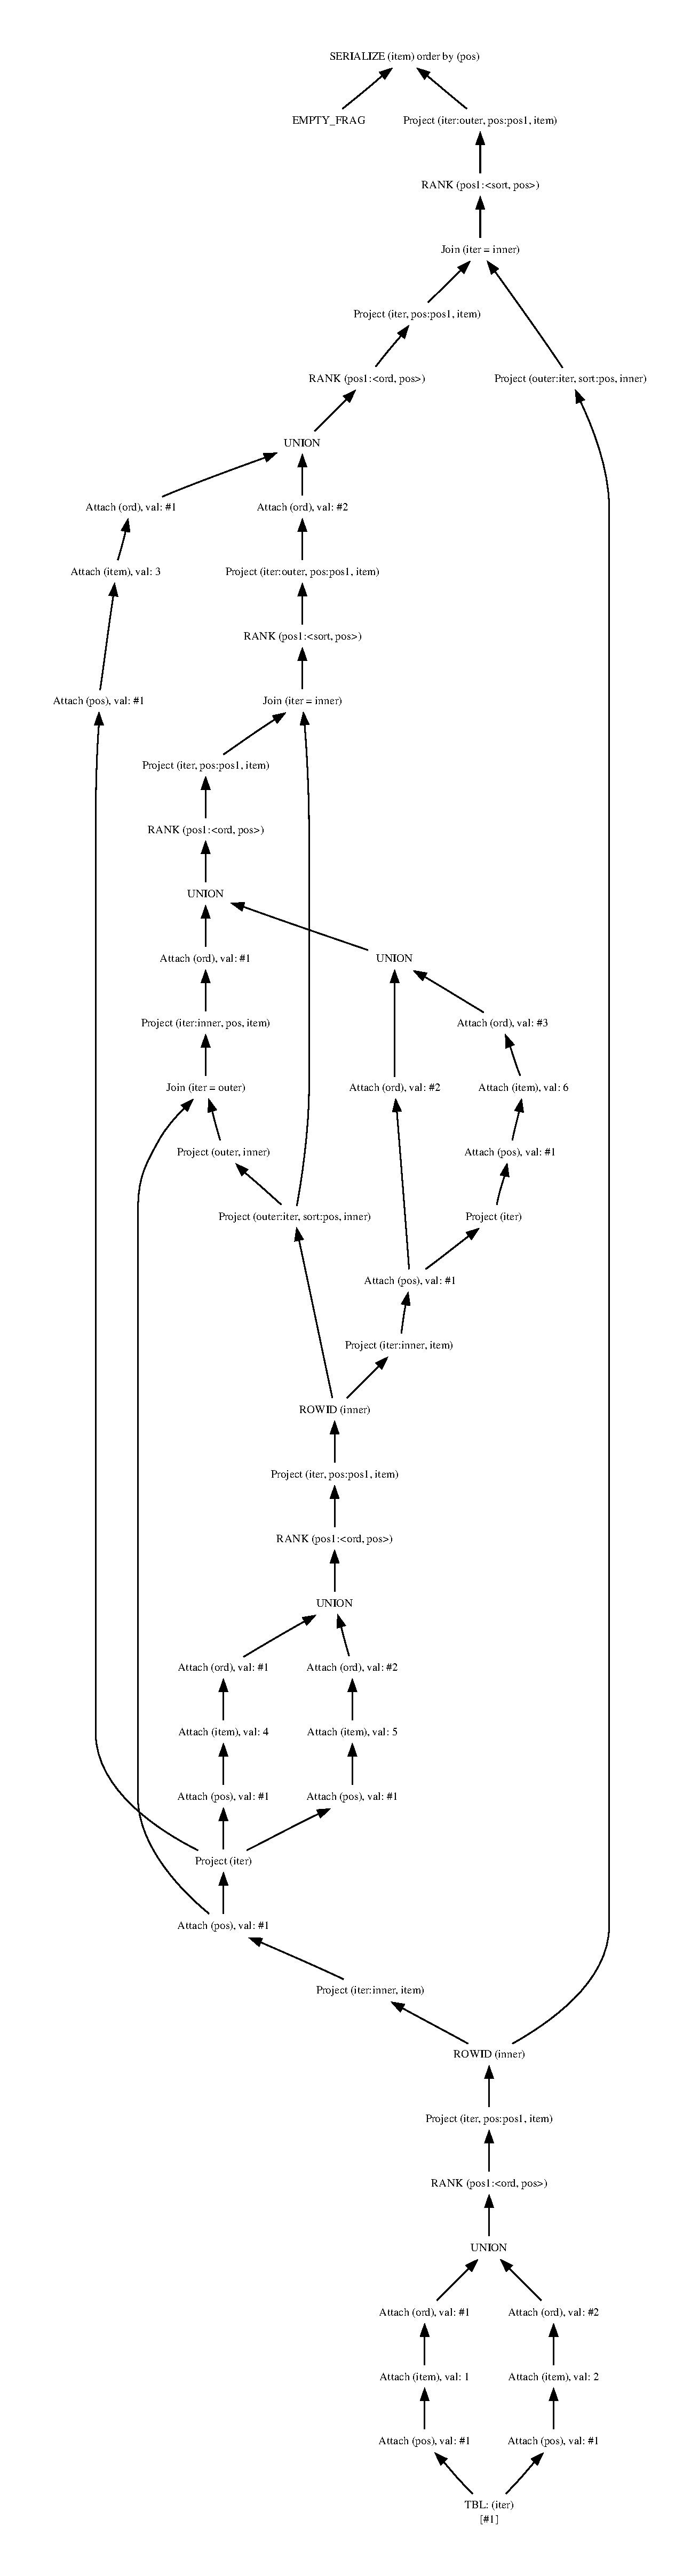
\includegraphics[width=0.37\textwidth]{img/graphs/td_impl_flwor_complex_pathfinder}
			\label{fig:result:comparison:complex_xqft_dag}
		}
		\quad
		\subfigure[Prototype implementation]{
		
			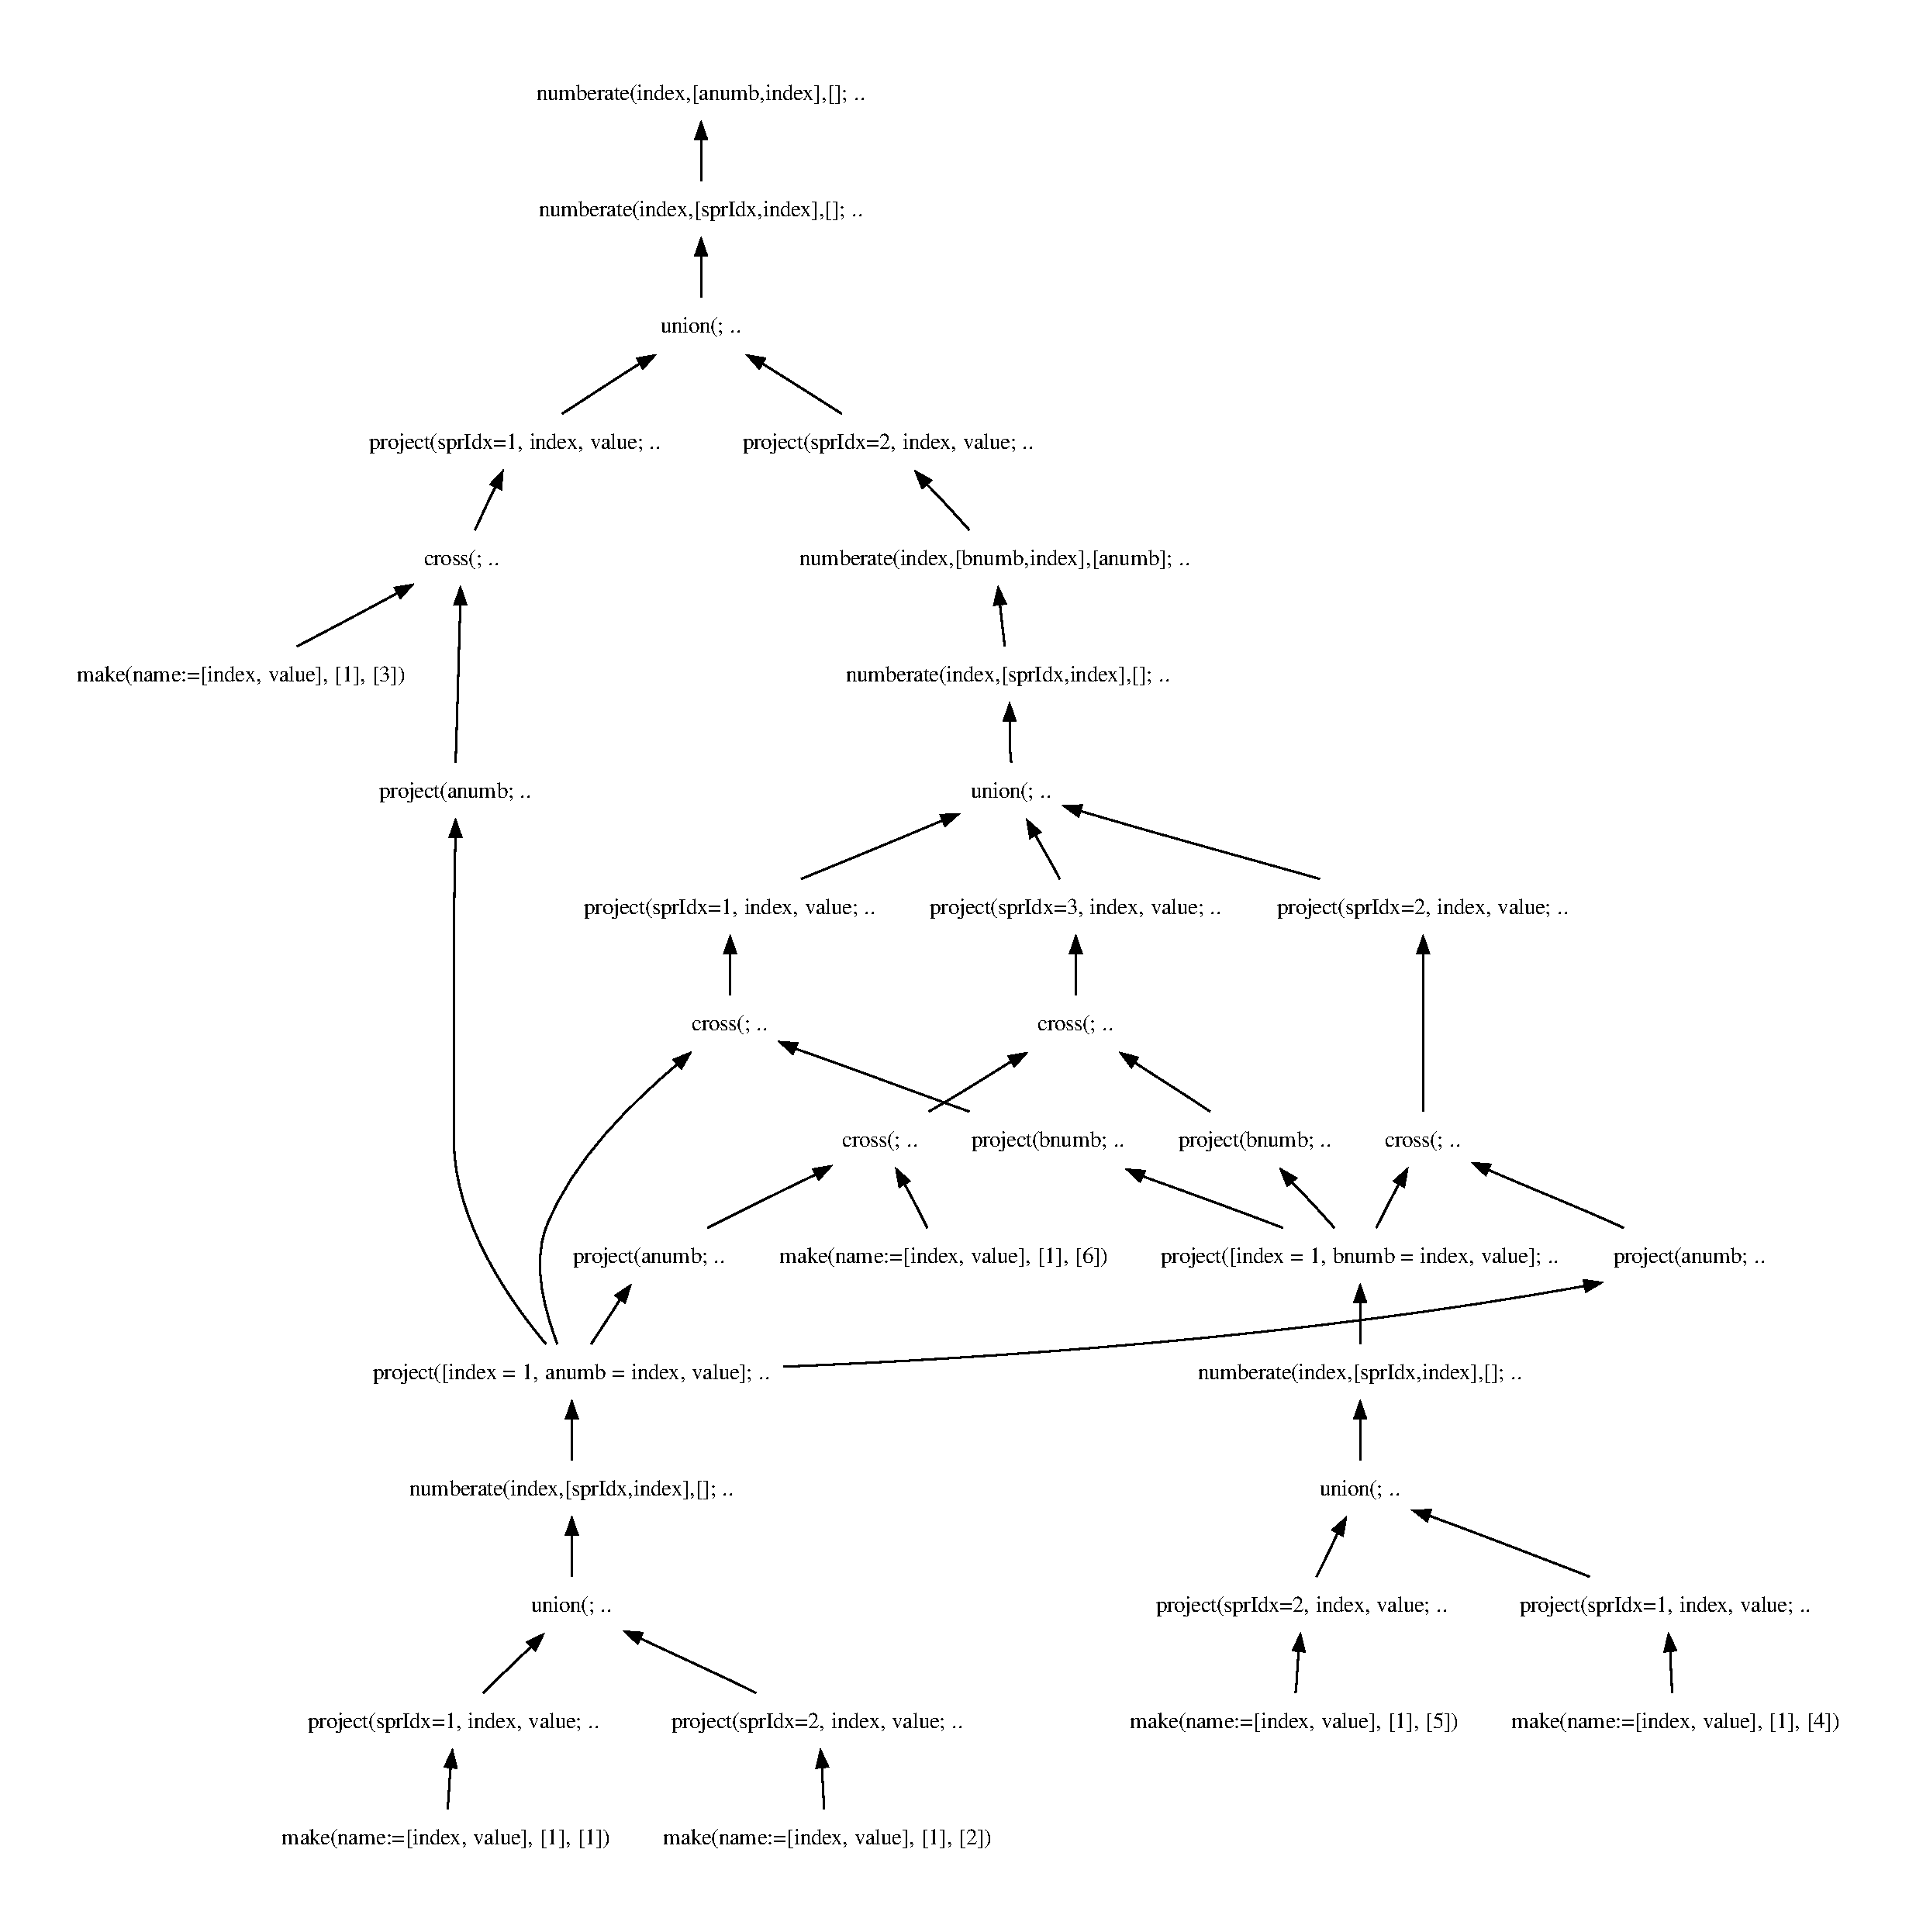
\includegraphics[width=0.6\textwidth]{img/graphs/td_impl_flwor_complex_xq_relalg_dag}
			\label{fig:result:comparison:complex_pathfinder_dag}
		}
	}
	\caption{Comparison of DAGs for the complex expression in section
	\ref{sect:results:algebra:generated:complex_flwor}}
\end{figure}

\newpage
\subsection{Complexity estimation and comparison}
Complexity estimation is performed as detailed in section
\ref{sect:method:complexity}. The complexity
comparison matrix is shown in table \ref{table:result:complexity_matrix}.

\begin{table}[!htp]
 \begin{center} 
 \begin{tabular}{| c | c | c || c | c |}
  \hline
   & \multicolumn{2}{|c||}{\textbf{Pathfinder/MonetDB}}
   & \multicolumn{2}{|c|}{\textbf{Prototype implementation}} \\
   \hline
   & Tuples & Fields & Tuples & Fields \\  
   \hline
   Trivial & 16 & 16 & 15 & 18 \\  
   \hline
   Complex & 215 & 265 & 136 & 102 \\
   \hline
   Conditional & 94 & 50 & 31 & 44 \\  
   \hline
 \end{tabular}
\caption{Complexity comparison matrix}
\label{table:result:complexity_matrix}
 \end{center}
\end{table}




\begin{figure}[!htp]
\begin{center}
  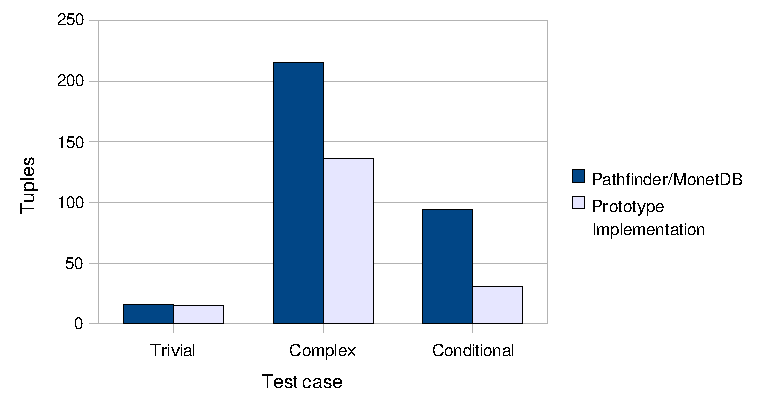
\includegraphics[width=1.0\textwidth]{diagrams/comparison_chart2_chart1}
  \caption{Comparison of complexity based on tuple creation}
  \label{fig:results:comparison:chart1}
\end{center}
\end{figure}

\begin{figure}[!htp]
\begin{center}
  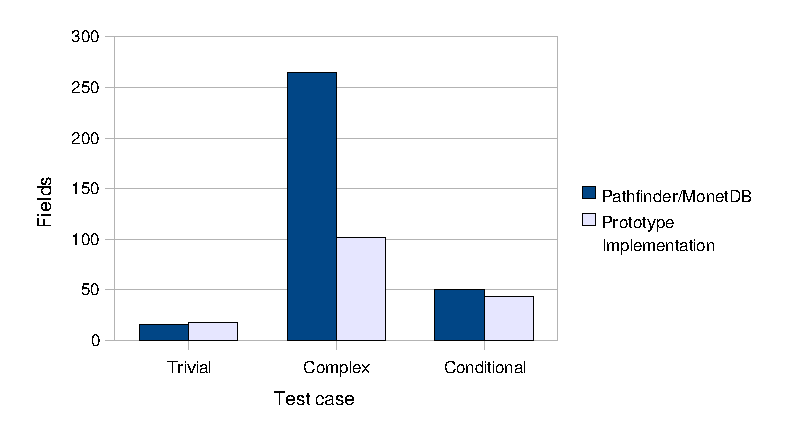
\includegraphics[width=1.0\textwidth]{diagrams/comparison_chart2_chart2}
  \caption{Comparison of complexity based on field creation}
  \label{fig:results:comparison:chart2}
\end{center}
\end{figure}

% Joins
\begin{table}[!htp]
 \begin{center}
 \begin{tabular}{| c | c | c | c | c | c | c | c |}
  \hline
   & \multicolumn{7}{|c|}{\textbf{Pathfinder}} \\
   \hline
   &  & \multicolumn{3}{|c|}{\textbf{In}} &
   \multicolumn{3}{|c|}{\textbf{Out}}  \\
   \hline
   &  \# & Min & Max & Avg & Min & Max & Avg\\
   \hline
   Trivial & 0 & 0 & 0 & 0 & 0 & 0 & 0  \\
   \hline
   Complex & 3 & 6 & 14 & 12.67 & 4 & 14 & 10  \\
   \hline
   Conditional & 3 & 4 & 6 & 4.67 & 1 & 2 & 1.67  \\
   \hline
   %\hline
   & \multicolumn{7}{|c|}{\textbf{Prototype}} \\
   \hline
   &  & \multicolumn{3}{|c|}{\textbf{In}} & 
   \multicolumn{3}{|c|}{\textbf{Out}} \\
   \hline
   & \# & Min & Max & Avg & Min & Max & Avg \\ 
   \hline 
   Trivial & 0 & 0 & 0 & 0 & 0 & 0 & 0 \\
   \hline
   Complex & 0 & 0 & 0 & 0 & 0 & 0 & 0 \\
   \hline
   Conditional & 2 & 3 & 6 & 4.5 & 3 & 6 & 4.5 \\
   \hline
 \end{tabular}
\caption{Tuple input/output in join operators}
\label{table:result:complexity_matrix}
 \end{center}
\end{table}


% Sorts
\begin{table}[!htp]
 \begin{center}
 \begin{tabular}{| c | c | c | c | c | c | c | c |}
  \hline
   & \multicolumn{7}{|c|}{\textbf{Pathfinder}} \\
   \hline
   &  & \multicolumn{3}{|c|}{\textbf{In}} &
   \multicolumn{3}{|c|}{\textbf{Out}}  \\
   \hline
   &  \# & Min & Max & Avg & Min & Max & Avg\\
   \hline
   Trivial & 1 & 3 & 3 & 3 & 3 & 3 & 3  \\
   \hline
   Complex & 6 & 2 & 14 & 8.8 & 2 & 14 & 8.8  \\
   \hline
   Conditional & 2 & 2 & 2 & 2 & 2 & 2 & 2  \\
   \hline
   %\hline
   & \multicolumn{7}{|c|}{\textbf{Prototype}} \\
   \hline
   &  & \multicolumn{3}{|c|}{\textbf{In}} &
   \multicolumn{3}{|c|}{\textbf{Out}} \\
   \hline
   & \# & Min & Max & Avg & Min & Max & Avg \\
   \hline
   Trivial & 2 & 3 & 3 & 3 & 3 & 3 & 3 \\
   \hline
   Complex & 6 & 2 & 14 & 9.33 & 2 & 14 & 9.33 \\
   \hline
   Conditional & 2 & 2 & 2 & 2 & 2 & 2 & 2 \\
   \hline
 \end{tabular}
\caption{Tuple input/output in join operators}
\label{table:result:complexity_matrix}
 \end{center}
\end{table}

\section{Summary}
\label{sect:res:summary}
\begin{itemize}
  \item sammendrag av dette kap
\end{itemize}

\chapter{Discussion}
\label{chapter:discussion}

\textbf{\underline{\LARGE TODO:}} innledning

\begin{itemize}
	\item Hva med \$i = (1,2,3) \$i/hatt -> typefeil? kj\o re isInScope(scope) p\aa~noe som ikke har scope kolonne?
\end{itemize}

\section{Loop Lift vs MarkXremove}
\label{sect:discussion:llvsmXr}
\begin{itemize}
  \item fordeler vs ulemper..
  \item dra frem at markXremove bruker f\ae rre operatorer
  \item men st\o tter ikke all verden -> fundamental feil? -> ordering iallefall, types ogs\aa~til en viss grad
  \item hva med en switch if(!all verden) -> markXremove else LoopL
  \item pathfinder way kommer ikke til \aa~dra nytte av den mer ekspressive mars-algebraen\ldots Men er ekspressiv
	  bedre? Synes jeg s\aa~ noe i en av pathfinder artiklene hvor de sa at jo mer restriktiv, jo bedre
	  \aa~optimisere\ldots snakke med thorbj\o rnsen om dette..
\end{itemize}

\section{Rewriting}
\label{sect:discussion:rewriting}
\begin{itemize}
  \item fordeler vs ulemper med \aa~skrive om til core
  \item man mister jo informasjon\ldots. Hvis den er p\aa~denne m\aa ten --> gj\o re det akkurat
	  slik, en sp\o rring som skal gi tilsvarende svar er ikke sikkert at man kan
	  skrive p\aa~den samme m\aa ten helt uten videre..  
  \item samme svar = samme utf\o relse = er dette en fordel?
  \item kan man utnytte kunnskap om translation til \aa~optimisere xquery queries?
  \item hva med \aa~bare skrive om det man trenger? Ala det vi gjorde med FLWORz?
\end{itemize}

\section{Manual vs. automated tree parser construction - {DROPPES?}}
ANTLR provides a utility for automated construction of AST parsers. This
utility requires the specification of a separate ``tree grammar''. This tree
grammar is almost identical to the original parser grammar. Practically, the
parser grammar can be copied verbatime, renamed, modified slightly and used as
a tree  grammar. This process is described in detail in \cite{definitiveAntlr},
section 8.1.

This introduces a high level of redundancy. The two grammar specifications are
required to be somewhat identical with regards to their grammar structure; that
is,  redundant tokens can be removed. However, the rewrite rules are required to
be identical.

This creates a problem with maintainability. As the parser grammar and rewrite
rules are not freezed at this point but rather highly subject to change, any
changes made in the parser grammar will need to be transferred to the tree
grammar, and vice versa. 

In \cite{translators_should_use_tree_grammars}, Terence Parr argues that the
traditional visitor
pattern\footnote{http://en.wikipedia.org/wiki/Visitor\_pattern} only provides a
simplistic facility for triggering events on the AST, that no tree structure
validation is implicitly available, and that context information has to be
passed down through the tree during the parse or by setting global variables.

In another point of view strongly polar to that of Terence Parr, Andy Tripp
argues\cite{manual_tree_walking_is_better} that manual tree parsing is
better. He establishes the following points of argument which are of particular
interest to this project:
\begin{itemize}
  \item Duplication of code and effort -- the concept of "what is a valid AST"
  would have to be implemented in both the parser and the AST transformer phase
  [as a rebuttal to validation of AST]
  \item With regards to contextual information, There seems to be nothing wrong
  with depending on the physical structure of the AST 
  \item Defining a traditional parser in grammar is practical because the grammar
  usually resembles the ouput AST. In the case of a tree parser proposed by Parr
  where the grammar actually resembles the input AST, this mapping may break
  down completely if the output is another tree structure
\end{itemize}

In particular, the last point holds a strong indication that a tree grammar
may not be suited for this project, as this tree parser will transform the AST
into a relational algebra tree.

\section{XQuery Features Not Supported - {MADS}}
\label{sect:disc:notSupported}
\textbf{\LARGE TODO: Mads}
\begin{itemize}
\item noen av disse tingene er ikke st\o tta pga typesystem, andre, slik som stemming og thesaurus er fordi ikkeno
slik i mars enn\aa~kan foresl\aa~det med parametere til lookup evt contextting ala \textsf{index()}.
  \item Dette avhenger jo seff av hvor mye vi har l\o st men disse b\o r kunne
  l\o ses:
  	\begin{itemize}
  		\item proximity (kanskje l\o sbar)
  		\item declare variable er nesten st\o tta\ldots men external og greier..
  		\item function declarations, b\o r g\aa~greit, bare ha en function table ala symbol table.
  		\item schema / schema validation -> typeting? Hvordan l\o ser pathfinder dette\ldots synes \aa~ha sett noe om
  		det\ldots
  		\item namespacezz\ldots.
  		\item node comparisons\ldots\ldots tviler p\aa~at vi f\aa r til dette glatt\ldots
  		\item order by med alle ting..
  		\item ordered and unordered -> lurer p\aa om (markXremove + tainting = TD uten $index$ og
  		\textsf{numberate()}) fikser dette ganske bra\ldots
  		\begin{itemize}
			\item MarkXRemove funker bra i unordered m0de tror jeg\ldots. Den er ogs\a~normalisert ref purely relational
			flwors, som sier LL er denormalisert. (bare normalisert innenfor en flwor.. den unormaliserer seg n\aa r den
			g\aa r ut av l\o kka (cross /m const))
			\item Order/unorder kan dra nytte av kontekstsensitive visitors\ldots\ldots
		\end{itemize}
  		\item \textbar, \texttt{union}, \texttt{intersect, except}
  		\item Range expressions $e_1$ \texttt{to} $e_2$ (begge m\aa~v\ae re integer tror jeg -> skrive om det i type?)
  		\item Prologs and modules
  		\item Quantified Expression: (some | every) \$b in $e_1$ satisfies $e_2$
  		\end{itemize}
	\end{itemize}

\subsection{Order By - {MADS}}
\label{sect:disc:orderby}
\textbf{\LARGE TODO: {MADS}}
\begin{itemize}
  \item st\o tte alle de sorteringsspesifiseringene.. st\o tte sortering over flere exprz.
\end{itemize}
	
	
	
	\subsection{XQuery Functions - {MADS}}
\label{sect:disc:functions}
\textbf{\LARGE TODO: {MADS}}
\begin{itemize}
  \item hvordan ordne XQuery funksjoner?
  \item Tror det skal v\ae re lagt til rette for \aa~ha en \textsf{function(FUNCTIONNAME; operator(list?)} operator
  \end{itemize}
  
fra 3.1.5:
\begin{quote}
  Additional functions may be declared in a Prolog, imported from a library module, or provided by the external
  environment as part of the static context.
  \end{quote}

\section{Predicates}
\label{sect:discussion:predicates}
\begin{itemize}
  \item saxon sier //ITEM[1] er to items fordi jeg har to BOOKS ? skal det ikke
  v\ae re 1 uansett?
  \item for stepexprz: 

	\begin{itemize}
	  \item de kan ikke sl\aa s sammen allikevel
	  \item hva med nummerering av rader, slik at man alltid kan bruke den hvis
	  predikatet er et tall?
	  \item kan v\ae re un\o dvendig siden man har instans-index i scope forh\aa
	  pentligvis..
	  \item flere relative pathexprs i predikater b\o r egentlig kunne mergeInJoines sammen f\o r de blir merginjoina
	  med det som predikatet st\aa r til\ldots dette er kanskje en optimalisering\ldots
    \end{itemize}
  \item for filterExprz:
  	\begin{itemize}
	  \item de eksisterer her ogs\aa~ja\ldots
	  \item hvordan l\o se dette generelt?
	  \item her m\aa~vi virkelig tenke p\aa~det med index iallefall\ldots 
	  \item ('a','b','c')[2] er lov
	  \item /a/b/c[1] er egentlig nesten mer unntaket enn reglen? Vanlig med
	  //c[1] regner jeg med.. og da blir det annerledes med en gang.. SCHADe
    \end{itemize} 
\end{itemize}

\section{Order}
\label{sect:discussion:order}
\begin{itemize}
  \item hva skjer om noe er sortert.. s\aa~blir det kryssa? M\aa~vi alltid gi ting ordernumber? Herregud s\aa~likt
  pathfinder i s\aa fall =/
  \item kanskje denne section og den om type kan sl\aa s sammen til noe om representering av data?
\end{itemize}

\section{Type System}
\label{sect:discussion:typeSystem}
\begin{itemize}
  \item Hvordan f\aa~til noe typesystem?
  \item Mars st\o tter ikke forskjellige typer innenfor samme felt
  \item En sekvens er en sekvens i XQuery\ldots ikke en sekvens av booleans
  eller noder etc
  \item Et ekstra felt som sier type?
  \item Hva skjer med /a/b/c/text() vs /a/b/c ?
  \item hva skjer om man lager en <a> hei <b> jeje </b> </a> variabel? Dette
  m\aa~kunne representeres.
\end{itemize}

\section{Optimisations}
\label{sect:discussion:optimisations}
\begin{itemize}
  \item legg merke til bruk av Uk-skrivem\aa te (s vs z)
  \item enkeltverdier i sammenligning b\o r bli putta inn i selecten.. ikke lag
  eget sett og kryss
  \item enkeltverdier etterhverandre b\o r lages i en go, ikke \texttt{union}es
  sammen
  \item step for step pathexpr er ikke effektivt\ldots SCHADE ulempe med rene uttrykk: /a/b/c = trengs ingen
  joins egentlig
  \item et step b\o r kanskje egentlig joines med konteksten sin f\o r predikatet sitt -> /a/b[c] ((a join a/b)
  join a/b/c) ikke (a join (a/b join /a/b/c)
  \item vi har ordna, uten \aa~vite om det at man kan selecte i stedet for \aa~projecte n\aa r man er i logisk
  kontekst.. yeah!
\end{itemize}
\chapter{Future Work}
\label{chapter:future}
\begin{itemize}	
  \item Sammenligne ytelse med Pathfinder n\aa r Fast har f\aa tt p\aa~plass en impl.
  \item Finne et typesystem (hvis ikke dette er gjort i l\o pet av Discussion)
  \item Finne mer simplifications og optimisations
\end{itemize}


\chapter{Conclusion}
\label{chapter:conclusion}
\begin{itemize}
  \item Vi har funnet opp metode
  \item Vi har implementert metoden
  \item vi har sammenlignet metoden
  \item vi har funnet ut at det kan hende vi er inne p\aa~noe
  \item \ldots
\end{itemize}
\appendix
\chapter{W3C Grammar}
Vi krymper det ned, s\aa ~f\aa r vi plass
\chapter{Antlr Grammar}
Vi krymper det ned, s\aa ~f\aa r vi plass
\bibliographystyle{plain}
\bibliography{references}
\end{document}